\documentclass[twoside]{book}

% Packages required by doxygen
\usepackage{fixltx2e}
\usepackage{calc}
\usepackage{doxygen}
\usepackage[export]{adjustbox} % also loads graphicx
\usepackage{graphicx}
\usepackage[utf8]{inputenc}
\usepackage{makeidx}
\usepackage{multicol}
\usepackage{multirow}
\PassOptionsToPackage{warn}{textcomp}
\usepackage{textcomp}
\usepackage[nointegrals]{wasysym}
\usepackage[table]{xcolor}

% NLS support packages
\usepackage{polski}
\usepackage[T1]{fontenc}

% Font selection
\usepackage[T1]{fontenc}
\usepackage[scaled=.90]{helvet}
\usepackage{courier}
\usepackage{amssymb}
\usepackage{sectsty}
\renewcommand{\familydefault}{\sfdefault}
\allsectionsfont{%
  \fontseries{bc}\selectfont%
  \color{darkgray}%
}
\renewcommand{\DoxyLabelFont}{%
  \fontseries{bc}\selectfont%
  \color{darkgray}%
}
\newcommand{\+}{\discretionary{\mbox{\scriptsize$\hookleftarrow$}}{}{}}

% Page & text layout
\usepackage{geometry}
\geometry{%
  a4paper,%
  top=2.5cm,%
  bottom=2.5cm,%
  left=2.5cm,%
  right=2.5cm%
}
\tolerance=750
\hfuzz=15pt
\hbadness=750
\setlength{\emergencystretch}{15pt}
\setlength{\parindent}{0cm}
\setlength{\parskip}{3ex plus 2ex minus 2ex}
\makeatletter
\renewcommand{\paragraph}{%
  \@startsection{paragraph}{4}{0ex}{-1.0ex}{1.0ex}{%
    \normalfont\normalsize\bfseries\SS@parafont%
  }%
}
\renewcommand{\subparagraph}{%
  \@startsection{subparagraph}{5}{0ex}{-1.0ex}{1.0ex}{%
    \normalfont\normalsize\bfseries\SS@subparafont%
  }%
}
\makeatother

% Headers & footers
\usepackage{fancyhdr}
\pagestyle{fancyplain}
\fancyhead[LE]{\fancyplain{}{\bfseries\thepage}}
\fancyhead[CE]{\fancyplain{}{}}
\fancyhead[RE]{\fancyplain{}{\bfseries\leftmark}}
\fancyhead[LO]{\fancyplain{}{\bfseries\rightmark}}
\fancyhead[CO]{\fancyplain{}{}}
\fancyhead[RO]{\fancyplain{}{\bfseries\thepage}}
\fancyfoot[LE]{\fancyplain{}{}}
\fancyfoot[CE]{\fancyplain{}{}}
\fancyfoot[RE]{\fancyplain{}{\bfseries\scriptsize Wygenerowano przez Doxygen }}
\fancyfoot[LO]{\fancyplain{}{\bfseries\scriptsize Wygenerowano przez Doxygen }}
\fancyfoot[CO]{\fancyplain{}{}}
\fancyfoot[RO]{\fancyplain{}{}}
\renewcommand{\footrulewidth}{0.4pt}
\renewcommand{\chaptermark}[1]{%
  \markboth{#1}{}%
}
\renewcommand{\sectionmark}[1]{%
  \markright{\thesection\ #1}%
}

% Indices & bibliography
\usepackage{natbib}
\usepackage[titles]{tocloft}
\setcounter{tocdepth}{3}
\setcounter{secnumdepth}{5}
\makeindex

% Hyperlinks (required, but should be loaded last)
\usepackage{ifpdf}
\ifpdf
  \usepackage[pdftex,pagebackref=true]{hyperref}
\else
  \usepackage[ps2pdf,pagebackref=true]{hyperref}
\fi
\hypersetup{%
  colorlinks=true,%
  linkcolor=blue,%
  citecolor=blue,%
  unicode%
}

% Custom commands
\newcommand{\clearemptydoublepage}{%
  \newpage{\pagestyle{empty}\cleardoublepage}%
}

\usepackage{caption}
\captionsetup{labelsep=space,justification=centering,font={bf},singlelinecheck=off,skip=4pt,position=top}

%===== C O N T E N T S =====

\begin{document}

% Titlepage & ToC
\hypersetup{pageanchor=false,
             bookmarksnumbered=true,
             pdfencoding=unicode
            }
\pagenumbering{alph}
\begin{titlepage}
\vspace*{7cm}
\begin{center}%
{\Large P\+R\+OI projekt 3 }\\
\vspace*{1cm}
{\large Wygenerowano przez Doxygen 1.8.13}\\
\end{center}
\end{titlepage}
\clearemptydoublepage
\pagenumbering{roman}
\tableofcontents
\clearemptydoublepage
\pagenumbering{arabic}
\hypersetup{pageanchor=true}

%--- Begin generated contents ---
\chapter{Algorytm podejmowania decyzji przez bota w grze}
\label{index}\hypertarget{index}{}\begin{DoxyAuthor}{Autor}
Bartłomiej Olber
\end{DoxyAuthor}
Gra w życie (Life, The game of life) – jeden z pierwszych i najbardziej znanych przykładów automatu komórkowego, wymyślony w roku 1970 przez brytyjskiego matematyka Johna Conwaya.

Gra toczy się na nieskończonej planszy (płaszczyźnie) podzielonej na kwadratowe komórki. Każda komórka ma ośmiu „sąsiadów” (tzw.\+sąsiedztwo Moore’a), czyli komórki przylegające do niej bokami i rogami. Każda komórka może znajdować się w jednym z dwóch stanów\+: może być albo „żywa” (wartość 1), albo „martwa” (wartość 0). Stany komórek zmieniają się w pewnych jednostkach czasu. Stan wszystkich komórek w pewnej jednostce czasu jest używany do obliczenia stanu wszystkich komórek w następnej jednostce. Po obliczeniu wszystkie komórki zmieniają swój stan dokładnie w tym samym momencie. Stan komórki zależy tylko od liczby jej żywych sąsiadów. W grze w życie nie ma graczy w dosłownym tego słowa znaczeniu. Udział człowieka sprowadza się jedynie do ustalenia stanu początkowego komórek.

{\bfseries Reguły gry według Conwaya} \begin{DoxyVerb}Martwa komórka, która ma dokładnie 3 żywych sąsiadów, staje się żywa 
w następnej jednostce czasu (rodzi się).
Żywa komórka z 2 albo 3 żywymi sąsiadami pozostaje nadal żywa; 
przy innej liczbie sąsiadów umiera (z „samotności” albo „zatłoczenia”).
\end{DoxyVerb}


{\bfseries Algorytmy programu}



{\bfseries Opcje programu} \begin{DoxyVerb}F1  Wyjdź z programu
F2  Wyświetl menu opcji użytkownika 
     - Ustaw żywe komórki na planszy
     - Ustaw maksymalną liczbę iteracji
     - Ustaw opóźnienie pomiędzy iteracjami
     - Ustaw rozmiary planszy 
     - Wylosuj stan planszy
F3  Zatrzymaj grę
F4  Strórz nową planszę
F9  Rozpocznij grę   
\end{DoxyVerb}


{\bfseries Analiza pliku wejściowego}

Do analizy pliku wejściowego typu J\+S\+ON została użyta biblioteka Y\+A\+JL.

Oto przykład poprawnego pliku parametrów typu J\+S\+ON

 
\chapter{Indeks hierarchiczny}
\section{Hierarchia klas}
Ta lista dziedziczenia posortowana jest z grubsza, choć nie całkowicie, alfabetycznie\+:\begin{DoxyCompactList}
\item \contentsline{section}{model\+:\+:Action}{\pageref{classmodel_1_1Action}}{}
\begin{DoxyCompactList}
\item \contentsline{section}{model\+:\+:Castle\+Action}{\pageref{classmodel_1_1CastleAction}}{}
\begin{DoxyCompactList}
\item \contentsline{section}{model\+:\+:Build\+High\+Tier\+Action}{\pageref{classmodel_1_1BuildHighTierAction}}{}
\item \contentsline{section}{model\+:\+:Build\+Low\+Tier\+Action}{\pageref{classmodel_1_1BuildLowTierAction}}{}
\item \contentsline{section}{model\+:\+:Build\+Mid\+Tier\+Action}{\pageref{classmodel_1_1BuildMidTierAction}}{}
\item \contentsline{section}{model\+:\+:Recruit\+High\+Tier\+Action}{\pageref{classmodel_1_1RecruitHighTierAction}}{}
\item \contentsline{section}{model\+:\+:Recruit\+Low\+Tier\+Action}{\pageref{classmodel_1_1RecruitLowTierAction}}{}
\item \contentsline{section}{model\+:\+:Recruit\+Mid\+Tier\+Action}{\pageref{classmodel_1_1RecruitMidTierAction}}{}
\end{DoxyCompactList}
\item \contentsline{section}{model\+:\+:Hero\+Action}{\pageref{classmodel_1_1HeroAction}}{}
\begin{DoxyCompactList}
\item \contentsline{section}{model\+:\+:Enter\+Action}{\pageref{classmodel_1_1EnterAction}}{}
\item \contentsline{section}{model\+:\+:Fight\+Action}{\pageref{classmodel_1_1FightAction}}{}
\item \contentsline{section}{model\+:\+:Pick\+Up\+Action}{\pageref{classmodel_1_1PickUpAction}}{}
\item \contentsline{section}{model\+:\+:Travel\+To\+Action}{\pageref{classmodel_1_1TravelToAction}}{}
\end{DoxyCompactList}
\end{DoxyCompactList}
\item \contentsline{section}{bot\+:\+:Action\+Executor}{\pageref{classbot_1_1ActionExecutor}}{}
\item \contentsline{section}{brain\+:\+:Brain}{\pageref{classbrain_1_1Brain}}{}
\item \contentsline{section}{model\+:\+:Game\+Object}{\pageref{classmodel_1_1GameObject}}{}
\begin{DoxyCompactList}
\item \contentsline{section}{model\+:\+:Army}{\pageref{classmodel_1_1Army}}{}
\item \contentsline{section}{model\+:\+:Building}{\pageref{classmodel_1_1Building}}{}
\begin{DoxyCompactList}
\item \contentsline{section}{model\+:\+:Guarded\+Building}{\pageref{classmodel_1_1GuardedBuilding}}{}
\end{DoxyCompactList}
\item \contentsline{section}{model\+:\+:Castle}{\pageref{classmodel_1_1Castle}}{}
\item \contentsline{section}{model\+:\+:Gold}{\pageref{classmodel_1_1Gold}}{}
\item \contentsline{section}{model\+:\+:Hero}{\pageref{classmodel_1_1Hero}}{}
\item \contentsline{section}{model\+:\+:Troop}{\pageref{classmodel_1_1Troop}}{}
\end{DoxyCompactList}
\item \contentsline{section}{model\+:\+:Game\+State}{\pageref{structmodel_1_1GameState}}{}
\item \contentsline{section}{bot\+:\+:Screen\+Capture}{\pageref{classbot_1_1ScreenCapture}}{}
\item \contentsline{section}{model\+:\+:Status\+Converter}{\pageref{classmodel_1_1StatusConverter}}{}
\item \contentsline{section}{model\+:\+:Tier\+Converter}{\pageref{classmodel_1_1TierConverter}}{}
\end{DoxyCompactList}

\chapter{Indeks klas}
\section{Lista klas}
Tutaj znajdują się klasy, struktury, unie i interfejsy wraz z ich krótkimi opisami\+:\begin{DoxyCompactList}
\item\contentsline{section}{\hyperlink{classmodel_1_1Action}{model\+::\+Action} \\*Klasa \hyperlink{classmodel_1_1Action}{Action} }{\pageref{classmodel_1_1Action}}{}
\item\contentsline{section}{\hyperlink{classbot_1_1ActionExecutor}{bot\+::\+Action\+Executor} \\*Klasa \hyperlink{classbot_1_1ActionExecutor}{Action\+Executor} }{\pageref{classbot_1_1ActionExecutor}}{}
\item\contentsline{section}{\hyperlink{classmodel_1_1Army}{model\+::\+Army} \\*Klasa \hyperlink{classmodel_1_1Army}{Army} }{\pageref{classmodel_1_1Army}}{}
\item\contentsline{section}{\hyperlink{classbrain_1_1Brain}{brain\+::\+Brain} \\*Klasa \hyperlink{classbrain_1_1Brain}{Brain} }{\pageref{classbrain_1_1Brain}}{}
\item\contentsline{section}{\hyperlink{classmodel_1_1BuildHighTierAction}{model\+::\+Build\+High\+Tier\+Action} \\*Klasa \hyperlink{classmodel_1_1BuildHighTierAction}{Build\+High\+Tier\+Action} }{\pageref{classmodel_1_1BuildHighTierAction}}{}
\item\contentsline{section}{\hyperlink{classmodel_1_1Building}{model\+::\+Building} \\*Klasa \hyperlink{classmodel_1_1Building}{Building} }{\pageref{classmodel_1_1Building}}{}
\item\contentsline{section}{\hyperlink{classmodel_1_1BuildLowTierAction}{model\+::\+Build\+Low\+Tier\+Action} \\*Klasa \hyperlink{classmodel_1_1BuildLowTierAction}{Build\+Low\+Tier\+Action} }{\pageref{classmodel_1_1BuildLowTierAction}}{}
\item\contentsline{section}{\hyperlink{classmodel_1_1BuildMidTierAction}{model\+::\+Build\+Mid\+Tier\+Action} \\*Klasa \hyperlink{classmodel_1_1BuildMidTierAction}{Build\+Mid\+Tier\+Action} }{\pageref{classmodel_1_1BuildMidTierAction}}{}
\item\contentsline{section}{\hyperlink{classmodel_1_1Castle}{model\+::\+Castle} \\*Klasa \hyperlink{classmodel_1_1Castle}{Castle} }{\pageref{classmodel_1_1Castle}}{}
\item\contentsline{section}{\hyperlink{classmodel_1_1CastleAction}{model\+::\+Castle\+Action} \\*Klasa \hyperlink{classmodel_1_1CastleAction}{Castle\+Action} }{\pageref{classmodel_1_1CastleAction}}{}
\item\contentsline{section}{\hyperlink{classmodel_1_1EnterAction}{model\+::\+Enter\+Action} \\*Klasa \hyperlink{classmodel_1_1EnterAction}{Enter\+Action} }{\pageref{classmodel_1_1EnterAction}}{}
\item\contentsline{section}{\hyperlink{classmodel_1_1FightAction}{model\+::\+Fight\+Action} \\*Klasa \hyperlink{classmodel_1_1FightAction}{Fight\+Action} }{\pageref{classmodel_1_1FightAction}}{}
\item\contentsline{section}{\hyperlink{classmodel_1_1GameObject}{model\+::\+Game\+Object} \\*Klasa \hyperlink{classmodel_1_1GameObject}{Game\+Object} }{\pageref{classmodel_1_1GameObject}}{}
\item\contentsline{section}{\hyperlink{structmodel_1_1GameState}{model\+::\+Game\+State} \\*Struktura \hyperlink{structmodel_1_1GameState}{Game\+State} }{\pageref{structmodel_1_1GameState}}{}
\item\contentsline{section}{\hyperlink{classmodel_1_1Gold}{model\+::\+Gold} \\*Klasa \hyperlink{classmodel_1_1Gold}{Gold} }{\pageref{classmodel_1_1Gold}}{}
\item\contentsline{section}{\hyperlink{classmodel_1_1GuardedBuilding}{model\+::\+Guarded\+Building} \\*Klasa \hyperlink{classmodel_1_1GuardedBuilding}{Guarded\+Building} }{\pageref{classmodel_1_1GuardedBuilding}}{}
\item\contentsline{section}{\hyperlink{classmodel_1_1Hero}{model\+::\+Hero} \\*Klasa \hyperlink{classmodel_1_1Hero}{Hero} }{\pageref{classmodel_1_1Hero}}{}
\item\contentsline{section}{\hyperlink{classmodel_1_1HeroAction}{model\+::\+Hero\+Action} \\*Klasa \hyperlink{classmodel_1_1HeroAction}{Hero\+Action} }{\pageref{classmodel_1_1HeroAction}}{}
\item\contentsline{section}{\hyperlink{classmodel_1_1PickUpAction}{model\+::\+Pick\+Up\+Action} \\*Klasa \hyperlink{classmodel_1_1PickUpAction}{Pick\+Up\+Action} }{\pageref{classmodel_1_1PickUpAction}}{}
\item\contentsline{section}{\hyperlink{classmodel_1_1RecruitHighTierAction}{model\+::\+Recruit\+High\+Tier\+Action} \\*Klasa \hyperlink{classmodel_1_1RecruitHighTierAction}{Recruit\+High\+Tier\+Action} }{\pageref{classmodel_1_1RecruitHighTierAction}}{}
\item\contentsline{section}{\hyperlink{classmodel_1_1RecruitLowTierAction}{model\+::\+Recruit\+Low\+Tier\+Action} \\*Klasa \hyperlink{classmodel_1_1RecruitLowTierAction}{Recruit\+Low\+Tier\+Action} }{\pageref{classmodel_1_1RecruitLowTierAction}}{}
\item\contentsline{section}{\hyperlink{classmodel_1_1RecruitMidTierAction}{model\+::\+Recruit\+Mid\+Tier\+Action} \\*Klasa \hyperlink{classmodel_1_1RecruitMidTierAction}{Recruit\+Mid\+Tier\+Action} }{\pageref{classmodel_1_1RecruitMidTierAction}}{}
\item\contentsline{section}{\hyperlink{classbot_1_1ScreenCapture}{bot\+::\+Screen\+Capture} \\*Klasa \hyperlink{classbot_1_1ScreenCapture}{Screen\+Capture} }{\pageref{classbot_1_1ScreenCapture}}{}
\item\contentsline{section}{\hyperlink{classmodel_1_1StatusConverter}{model\+::\+Status\+Converter} \\*Klasa \hyperlink{classmodel_1_1StatusConverter}{Status\+Converter} }{\pageref{classmodel_1_1StatusConverter}}{}
\item\contentsline{section}{\hyperlink{classmodel_1_1TierConverter}{model\+::\+Tier\+Converter} \\*Klasa \hyperlink{classmodel_1_1TierConverter}{Tier\+Converter} }{\pageref{classmodel_1_1TierConverter}}{}
\item\contentsline{section}{\hyperlink{classmodel_1_1TravelToAction}{model\+::\+Travel\+To\+Action} \\*Klasa \hyperlink{classmodel_1_1TravelToAction}{Travel\+To\+Action} }{\pageref{classmodel_1_1TravelToAction}}{}
\item\contentsline{section}{\hyperlink{classmodel_1_1Troop}{model\+::\+Troop} \\*Klasa \hyperlink{classmodel_1_1Troop}{Troop} }{\pageref{classmodel_1_1Troop}}{}
\end{DoxyCompactList}

\chapter{Indeks plików}
\section{Lista plików}
Tutaj znajduje się lista wszystkich udokumentowanych plików z ich krótkimi opisami\+:\begin{DoxyCompactList}
\item\contentsline{section}{/home/bartlomiej/eclipse-\/workspace/lab\+\_\+3/src/bot/\hyperlink{action__executor_8hpp}{action\+\_\+executor.\+hpp} \\*Moduł klasy Action\+Executor }{\pageref{action__executor_8hpp}}{}
\item\contentsline{section}{/home/bartlomiej/eclipse-\/workspace/lab\+\_\+3/src/bot/\hyperlink{brain_8hpp}{brain.\+hpp} \\*Moduł klasy Brain }{\pageref{brain_8hpp}}{}
\item\contentsline{section}{/home/bartlomiej/eclipse-\/workspace/lab\+\_\+3/src/bot/\hyperlink{screen__capture_8hpp}{screen\+\_\+capture.\+hpp} \\*Moduł klasy Screen\+Capture }{\pageref{screen__capture_8hpp}}{}
\item\contentsline{section}{/home/bartlomiej/eclipse-\/workspace/lab\+\_\+3/src/bot/model/\hyperlink{action_8hpp}{action.\+hpp} \\*Moduł klasy Action }{\pageref{action_8hpp}}{}
\item\contentsline{section}{/home/bartlomiej/eclipse-\/workspace/lab\+\_\+3/src/bot/model/\hyperlink{army_8hpp}{army.\+hpp} \\*Moduł klasy Army }{\pageref{army_8hpp}}{}
\item\contentsline{section}{/home/bartlomiej/eclipse-\/workspace/lab\+\_\+3/src/bot/model/\hyperlink{build__high__tier__action_8hpp}{build\+\_\+high\+\_\+tier\+\_\+action.\+hpp} \\*Moduł klasy Build\+High\+Tier\+Action }{\pageref{build__high__tier__action_8hpp}}{}
\item\contentsline{section}{/home/bartlomiej/eclipse-\/workspace/lab\+\_\+3/src/bot/model/\hyperlink{build__low__tier__action_8hpp}{build\+\_\+low\+\_\+tier\+\_\+action.\+hpp} \\*Moduł klasy Build\+Low\+Tier\+Action }{\pageref{build__low__tier__action_8hpp}}{}
\item\contentsline{section}{/home/bartlomiej/eclipse-\/workspace/lab\+\_\+3/src/bot/model/\hyperlink{build__mid__tier__action_8hpp}{build\+\_\+mid\+\_\+tier\+\_\+action.\+hpp} \\*Moduł klasy Build\+Mid\+Tier\+Action }{\pageref{build__mid__tier__action_8hpp}}{}
\item\contentsline{section}{/home/bartlomiej/eclipse-\/workspace/lab\+\_\+3/src/bot/model/\hyperlink{building_8hpp}{building.\+hpp} \\*Moduł klasy Building }{\pageref{building_8hpp}}{}
\item\contentsline{section}{/home/bartlomiej/eclipse-\/workspace/lab\+\_\+3/src/bot/model/\hyperlink{castle_8hpp}{castle.\+hpp} \\*Moduł klasy Castle }{\pageref{castle_8hpp}}{}
\item\contentsline{section}{/home/bartlomiej/eclipse-\/workspace/lab\+\_\+3/src/bot/model/\hyperlink{castle__actions_8hpp}{castle\+\_\+actions.\+hpp} \\*Moduł klasy Castle\+Action }{\pageref{castle__actions_8hpp}}{}
\item\contentsline{section}{/home/bartlomiej/eclipse-\/workspace/lab\+\_\+3/src/bot/model/\hyperlink{enter__action_8hpp}{enter\+\_\+action.\+hpp} \\*Moduł klasy Enter\+Action }{\pageref{enter__action_8hpp}}{}
\item\contentsline{section}{/home/bartlomiej/eclipse-\/workspace/lab\+\_\+3/src/bot/model/\hyperlink{fight__action_8hpp}{fight\+\_\+action.\+hpp} \\*Moduł klasy Fight\+Action }{\pageref{fight__action_8hpp}}{}
\item\contentsline{section}{/home/bartlomiej/eclipse-\/workspace/lab\+\_\+3/src/bot/model/\hyperlink{game__object_8hpp}{game\+\_\+object.\+hpp} \\*Moduł klasy Game\+Object }{\pageref{game__object_8hpp}}{}
\item\contentsline{section}{/home/bartlomiej/eclipse-\/workspace/lab\+\_\+3/src/bot/model/\hyperlink{game__state_8hpp}{game\+\_\+state.\+hpp} \\*Moduł klasy Game\+State }{\pageref{game__state_8hpp}}{}
\item\contentsline{section}{/home/bartlomiej/eclipse-\/workspace/lab\+\_\+3/src/bot/model/\hyperlink{gold_8hpp}{gold.\+hpp} \\*Moduł klasy Gold }{\pageref{gold_8hpp}}{}
\item\contentsline{section}{/home/bartlomiej/eclipse-\/workspace/lab\+\_\+3/src/bot/model/\hyperlink{guarded__building_8hpp}{guarded\+\_\+building.\+hpp} \\*Moduł klasy Guarded\+Building }{\pageref{guarded__building_8hpp}}{}
\item\contentsline{section}{/home/bartlomiej/eclipse-\/workspace/lab\+\_\+3/src/bot/model/\hyperlink{hero_8hpp}{hero.\+hpp} \\*Moduł klasy Hero }{\pageref{hero_8hpp}}{}
\item\contentsline{section}{/home/bartlomiej/eclipse-\/workspace/lab\+\_\+3/src/bot/model/\hyperlink{hero__action_8hpp}{hero\+\_\+action.\+hpp} \\*Moduł klasy Hero\+Action }{\pageref{hero__action_8hpp}}{}
\item\contentsline{section}{/home/bartlomiej/eclipse-\/workspace/lab\+\_\+3/src/bot/model/\hyperlink{pick__up__action_8hpp}{pick\+\_\+up\+\_\+action.\+hpp} \\*Moduł klasy Pick\+Up\+Action }{\pageref{pick__up__action_8hpp}}{}
\item\contentsline{section}{/home/bartlomiej/eclipse-\/workspace/lab\+\_\+3/src/bot/model/\hyperlink{recruit__high__tier__action_8hpp}{recruit\+\_\+high\+\_\+tier\+\_\+action.\+hpp} \\*Moduł klasy Recruit\+High\+Tier\+Action }{\pageref{recruit__high__tier__action_8hpp}}{}
\item\contentsline{section}{/home/bartlomiej/eclipse-\/workspace/lab\+\_\+3/src/bot/model/\hyperlink{recruit__low__tier__action_8hpp}{recruit\+\_\+low\+\_\+tier\+\_\+action.\+hpp} \\*Moduł klasy Recruit\+Low\+Tier\+Action }{\pageref{recruit__low__tier__action_8hpp}}{}
\item\contentsline{section}{/home/bartlomiej/eclipse-\/workspace/lab\+\_\+3/src/bot/model/\hyperlink{recruit__mid__tier__action_8hpp}{recruit\+\_\+mid\+\_\+tier\+\_\+action.\+hpp} \\*Moduł klasy Recruit\+Mid\+Tier\+Action }{\pageref{recruit__mid__tier__action_8hpp}}{}
\item\contentsline{section}{/home/bartlomiej/eclipse-\/workspace/lab\+\_\+3/src/bot/model/\hyperlink{status_8hpp}{status.\+hpp} \\*Moduł klasy enumeracyjnej Status i klasy konwertera Status\+Converter }{\pageref{status_8hpp}}{}
\item\contentsline{section}{/home/bartlomiej/eclipse-\/workspace/lab\+\_\+3/src/bot/model/\hyperlink{tier_8hpp}{tier.\+hpp} \\*Moduł klasy enumeracyjnej Tier i klasy konwertera Tier\+Converter }{\pageref{tier_8hpp}}{}
\item\contentsline{section}{/home/bartlomiej/eclipse-\/workspace/lab\+\_\+3/src/bot/model/\hyperlink{travel__to__action_8hpp}{travel\+\_\+to\+\_\+action.\+hpp} \\*Moduł klasy Travel\+To\+Action }{\pageref{travel__to__action_8hpp}}{}
\item\contentsline{section}{/home/bartlomiej/eclipse-\/workspace/lab\+\_\+3/src/bot/model/\hyperlink{troop_8hpp}{troop.\+hpp} \\*Moduł klasy Troop }{\pageref{troop_8hpp}}{}
\end{DoxyCompactList}

\chapter{Dokumentacja klas}
\hypertarget{classmodel_1_1Action}{}\section{Dokumentacja klasy model\+:\+:Action}
\label{classmodel_1_1Action}\index{model\+::\+Action@{model\+::\+Action}}


Klasa \hyperlink{classmodel_1_1Action}{Action}.  




{\ttfamily \#include $<$action.\+hpp$>$}



Diagram dziedziczenia dla model\+:\+:Action\nopagebreak
\begin{figure}[H]
\begin{center}
\leavevmode
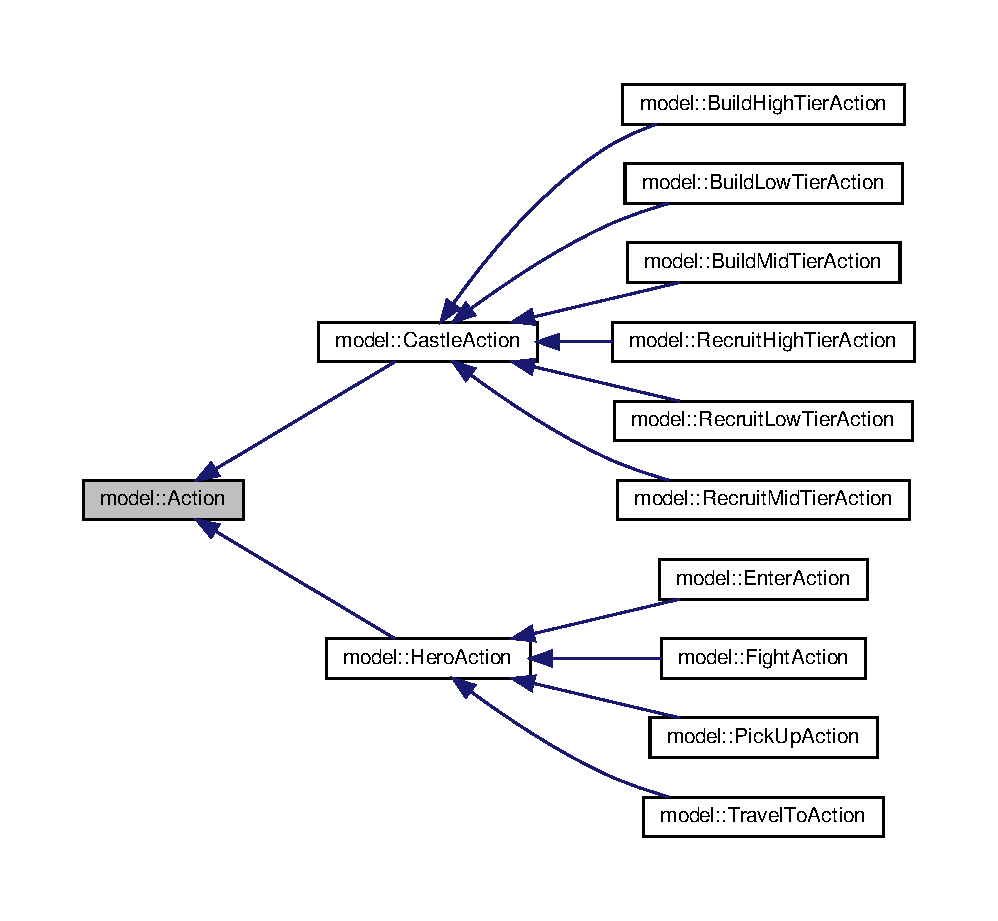
\includegraphics[width=350pt]{classmodel_1_1Action__inherit__graph}
\end{center}
\end{figure}


Diagram współpracy dla model\+:\+:Action\+:\nopagebreak
\begin{figure}[H]
\begin{center}
\leavevmode
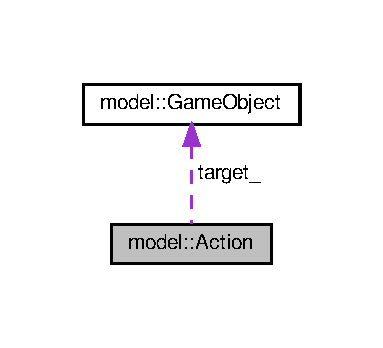
\includegraphics[width=184pt]{classmodel_1_1Action__coll__graph}
\end{center}
\end{figure}
\subsection*{Metody publiczne}
\begin{DoxyCompactItemize}
\item 
\hyperlink{classmodel_1_1Action_a0c62dc2f134f0feb4bc1eb5ac9ce5e67}{Action} (const \hyperlink{classmodel_1_1GameObject}{Game\+Object} \&target)
\begin{DoxyCompactList}\small\item\em Publiczny konstruktor z parametrem klasy \hyperlink{classmodel_1_1GameObject}{Game\+Object}. \end{DoxyCompactList}\item 
\hyperlink{classmodel_1_1Action_a0293d4a2d9f4bd4bf9f6b4427f83d531}{Action} (int x, int y)
\begin{DoxyCompactList}\small\item\em Publiczny konstruktor z parametrami integer. \end{DoxyCompactList}\item 
\mbox{\Hypertarget{classmodel_1_1Action_a6c34264ee8e8ce12366b2b39b9397568}\label{classmodel_1_1Action_a6c34264ee8e8ce12366b2b39b9397568}} 
virtual \hyperlink{classmodel_1_1Action_a6c34264ee8e8ce12366b2b39b9397568}{$\sim$\+Action} ()
\begin{DoxyCompactList}\small\item\em Wirtualny destruktor. \end{DoxyCompactList}\item 
virtual void \hyperlink{classmodel_1_1Action_a2955dbb4a69e38a48aa07d730fe2d77c}{print} ()
\begin{DoxyCompactList}\small\item\em Wirtualna metoda print. \end{DoxyCompactList}\end{DoxyCompactItemize}
\subsection*{Atrybuty chronione}
\begin{DoxyCompactItemize}
\item 
\hyperlink{classmodel_1_1GameObject}{Game\+Object} \hyperlink{classmodel_1_1Action_aaa02d0e5308513cd6832c6cd1ac7157f}{target\+\_\+}
\begin{DoxyCompactList}\small\item\em Chroniona składowa klasy \hyperlink{classmodel_1_1GameObject}{Game\+Object}. \end{DoxyCompactList}\end{DoxyCompactItemize}


\subsection{Opis szczegółowy}
Klasa \hyperlink{classmodel_1_1Action}{Action}. 

Klasa imitująca klasę akcji wydanych przez algorytm bota. 

\subsection{Dokumentacja konstruktora i destruktora}
\mbox{\Hypertarget{classmodel_1_1Action_a0c62dc2f134f0feb4bc1eb5ac9ce5e67}\label{classmodel_1_1Action_a0c62dc2f134f0feb4bc1eb5ac9ce5e67}} 
\index{model\+::\+Action@{model\+::\+Action}!Action@{Action}}
\index{Action@{Action}!model\+::\+Action@{model\+::\+Action}}
\subsubsection{\texorpdfstring{Action()}{Action()}\hspace{0.1cm}{\footnotesize\ttfamily [1/2]}}
{\footnotesize\ttfamily model\+::\+Action\+::\+Action (\begin{DoxyParamCaption}\item[{const \hyperlink{classmodel_1_1GameObject}{Game\+Object} \&}]{target }\end{DoxyParamCaption})\hspace{0.3cm}{\ttfamily [inline]}, {\ttfamily [explicit]}}



Publiczny konstruktor z parametrem klasy \hyperlink{classmodel_1_1GameObject}{Game\+Object}. 


\begin{DoxyParams}{Parametry}
{\em target} & stała referencja na obiekt klasy \hyperlink{classmodel_1_1GameObject}{Game\+Object}. \\
\hline
\end{DoxyParams}
\mbox{\Hypertarget{classmodel_1_1Action_a0293d4a2d9f4bd4bf9f6b4427f83d531}\label{classmodel_1_1Action_a0293d4a2d9f4bd4bf9f6b4427f83d531}} 
\index{model\+::\+Action@{model\+::\+Action}!Action@{Action}}
\index{Action@{Action}!model\+::\+Action@{model\+::\+Action}}
\subsubsection{\texorpdfstring{Action()}{Action()}\hspace{0.1cm}{\footnotesize\ttfamily [2/2]}}
{\footnotesize\ttfamily model\+::\+Action\+::\+Action (\begin{DoxyParamCaption}\item[{int}]{x,  }\item[{int}]{y }\end{DoxyParamCaption})\hspace{0.3cm}{\ttfamily [inline]}, {\ttfamily [explicit]}}



Publiczny konstruktor z parametrami integer. 


\begin{DoxyParams}{Parametry}
{\em x} & integerowa współrzędna x. \\
\hline
{\em y} & integerowa współrzędna y. \\
\hline
\end{DoxyParams}


\subsection{Dokumentacja funkcji składowych}
\mbox{\Hypertarget{classmodel_1_1Action_a2955dbb4a69e38a48aa07d730fe2d77c}\label{classmodel_1_1Action_a2955dbb4a69e38a48aa07d730fe2d77c}} 
\index{model\+::\+Action@{model\+::\+Action}!print@{print}}
\index{print@{print}!model\+::\+Action@{model\+::\+Action}}
\subsubsection{\texorpdfstring{print()}{print()}}
{\footnotesize\ttfamily virtual void model\+::\+Action\+::print (\begin{DoxyParamCaption}{ }\end{DoxyParamCaption})\hspace{0.3cm}{\ttfamily [inline]}, {\ttfamily [virtual]}}



Wirtualna metoda print. 

Pusta metoda; w klasach pochodnych będzie służyć w celach jedynie informacyjnych. 

Reimplementowana w \hyperlink{classmodel_1_1BuildHighTierAction_a587f7c8efb015bbc00cb706e7e289edf}{model\+::\+Build\+High\+Tier\+Action}, \hyperlink{classmodel_1_1BuildLowTierAction_a0917c29053656d5914125a30bcd51cce}{model\+::\+Build\+Low\+Tier\+Action}, \hyperlink{classmodel_1_1BuildMidTierAction_abec06b6ae68325996228e9b36c9d05d3}{model\+::\+Build\+Mid\+Tier\+Action}, \hyperlink{classmodel_1_1EnterAction_a0e6f49b42a1c026c421f29193670abeb}{model\+::\+Enter\+Action}, \hyperlink{classmodel_1_1PickUpAction_a8e3d6499d8eb1f99566e0b5b3e6661c9}{model\+::\+Pick\+Up\+Action}, \hyperlink{classmodel_1_1RecruitLowTierAction_ac05d2ba4872e6b06bf3a218661a4abdc}{model\+::\+Recruit\+Low\+Tier\+Action}, \hyperlink{classmodel_1_1RecruitMidTierAction_a91d571781540c34eea70643518e4a33d}{model\+::\+Recruit\+Mid\+Tier\+Action}, \hyperlink{classmodel_1_1TravelToAction_accc5a7f3bf4d65e22d5d7d86624a8da1}{model\+::\+Travel\+To\+Action}, \hyperlink{classmodel_1_1FightAction_a416846e68a9aa998412da4d439dbc6cc}{model\+::\+Fight\+Action} i \hyperlink{classmodel_1_1RecruitHighTierAction_a0bedf8fdec991eff26a3eb9ffa5e552f}{model\+::\+Recruit\+High\+Tier\+Action}.



\subsection{Dokumentacja atrybutów składowych}
\mbox{\Hypertarget{classmodel_1_1Action_aaa02d0e5308513cd6832c6cd1ac7157f}\label{classmodel_1_1Action_aaa02d0e5308513cd6832c6cd1ac7157f}} 
\index{model\+::\+Action@{model\+::\+Action}!target\+\_\+@{target\+\_\+}}
\index{target\+\_\+@{target\+\_\+}!model\+::\+Action@{model\+::\+Action}}
\subsubsection{\texorpdfstring{target\+\_\+}{target\_}}
{\footnotesize\ttfamily \hyperlink{classmodel_1_1GameObject}{Game\+Object} model\+::\+Action\+::target\+\_\+\hspace{0.3cm}{\ttfamily [protected]}}



Chroniona składowa klasy \hyperlink{classmodel_1_1GameObject}{Game\+Object}. 

Jest to objekt, na którym akcja ma być wykonana. 

Dokumentacja dla tej klasy została wygenerowana z pliku\+:\begin{DoxyCompactItemize}
\item 
/home/bartlomiej/eclipse-\/workspace/lab\+\_\+3/src/bot/model/\hyperlink{action_8hpp}{action.\+hpp}\end{DoxyCompactItemize}

\hypertarget{classbot_1_1ActionExecutor}{}\section{Dokumentacja klasy bot\+:\+:Action\+Executor}
\label{classbot_1_1ActionExecutor}\index{bot\+::\+Action\+Executor@{bot\+::\+Action\+Executor}}


Klasa \hyperlink{classbot_1_1ActionExecutor}{Action\+Executor}.  




{\ttfamily \#include $<$action\+\_\+executor.\+hpp$>$}

\subsection*{Metody publiczne}
\begin{DoxyCompactItemize}
\item 
\hyperlink{classbot_1_1ActionExecutor_ae65d80e86469f29c5ad3794666b8d5c5}{Action\+Executor} (const \hyperlink{action_8hpp_a052d176abf53b10863680ac55e7ba40d}{model\+::\+Action\+Scenario} \&scenario)
\begin{DoxyCompactList}\small\item\em Publiczny konstruktor z parametrem klasy Action\+Scenario. \end{DoxyCompactList}\end{DoxyCompactItemize}


\subsection{Opis szczegółowy}
Klasa \hyperlink{classbot_1_1ActionExecutor}{Action\+Executor}. 

Pusta klasa imitująca klasę wykonawcy decyzji otrzymanych przez algorytm. 

\subsection{Dokumentacja konstruktora i destruktora}
\mbox{\Hypertarget{classbot_1_1ActionExecutor_ae65d80e86469f29c5ad3794666b8d5c5}\label{classbot_1_1ActionExecutor_ae65d80e86469f29c5ad3794666b8d5c5}} 
\index{bot\+::\+Action\+Executor@{bot\+::\+Action\+Executor}!Action\+Executor@{Action\+Executor}}
\index{Action\+Executor@{Action\+Executor}!bot\+::\+Action\+Executor@{bot\+::\+Action\+Executor}}
\subsubsection{\texorpdfstring{Action\+Executor()}{ActionExecutor()}}
{\footnotesize\ttfamily bot\+::\+Action\+Executor\+::\+Action\+Executor (\begin{DoxyParamCaption}\item[{const \hyperlink{action_8hpp_a052d176abf53b10863680ac55e7ba40d}{model\+::\+Action\+Scenario} \&}]{scenario }\end{DoxyParamCaption})\hspace{0.3cm}{\ttfamily [inline]}}



Publiczny konstruktor z parametrem klasy Action\+Scenario. 


\begin{DoxyParams}{Parametry}
{\em scenario} & stała referencja na obiekt klasy Action\+Scenario; scenariusz akcji do wykonania. \\
\hline
\end{DoxyParams}


Dokumentacja dla tej klasy została wygenerowana z pliku\+:\begin{DoxyCompactItemize}
\item 
/home/bartlomiej/eclipse-\/workspace/lab\+\_\+3/src/bot/\hyperlink{action__executor_8hpp}{action\+\_\+executor.\+hpp}\end{DoxyCompactItemize}

\hypertarget{classmodel_1_1Army}{}\section{Dokumentacja klasy model\+:\+:Army}
\label{classmodel_1_1Army}\index{model\+::\+Army@{model\+::\+Army}}


Klasa \hyperlink{classmodel_1_1Army}{Army}.  




{\ttfamily \#include $<$army.\+hpp$>$}



Diagram dziedziczenia dla model\+:\+:Army\nopagebreak
\begin{figure}[H]
\begin{center}
\leavevmode
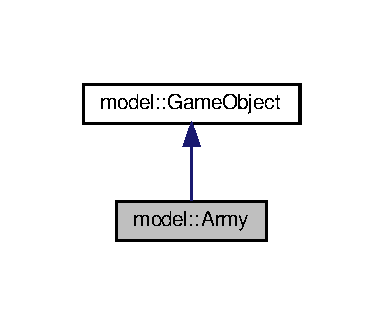
\includegraphics[width=184pt]{classmodel_1_1Army__inherit__graph}
\end{center}
\end{figure}


Diagram współpracy dla model\+:\+:Army\+:\nopagebreak
\begin{figure}[H]
\begin{center}
\leavevmode
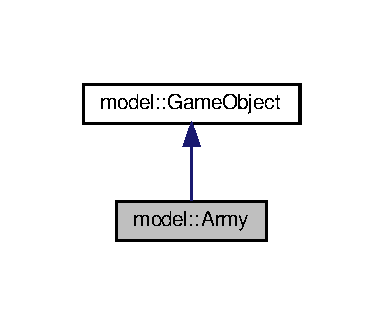
\includegraphics[width=184pt]{classmodel_1_1Army__coll__graph}
\end{center}
\end{figure}
\subsection*{Metody publiczne}
\begin{DoxyCompactItemize}
\item 
\hyperlink{classmodel_1_1Army_a09146560c4983f1d478cd490cc266333}{Army} (int high\+\_\+tier\+\_\+num, int mid\+\_\+tier\+\_\+num, int low\+\_\+tier\+\_\+num, int x, int y)
\begin{DoxyCompactList}\small\item\em Publiczny konstruktor z parametrami integerowymi. \end{DoxyCompactList}\item 
\mbox{\Hypertarget{classmodel_1_1Army_a81ae7bf335912170e9330ef27df6a450}\label{classmodel_1_1Army_a81ae7bf335912170e9330ef27df6a450}} 
int \hyperlink{classmodel_1_1Army_a81ae7bf335912170e9330ef27df6a450}{get\+\_\+high\+\_\+tier\+\_\+quantity} () const
\begin{DoxyCompactList}\small\item\em Getter zwraca liczbę jednostek wysokiego poziomu. \end{DoxyCompactList}\item 
\mbox{\Hypertarget{classmodel_1_1Army_a6845db50342d69bdcef1a215913fe316}\label{classmodel_1_1Army_a6845db50342d69bdcef1a215913fe316}} 
int \hyperlink{classmodel_1_1Army_a6845db50342d69bdcef1a215913fe316}{get\+\_\+mid\+\_\+tier\+\_\+quantity} () const
\begin{DoxyCompactList}\small\item\em Getter zwraca liczbę jednostek średniego poziomu. \end{DoxyCompactList}\item 
\mbox{\Hypertarget{classmodel_1_1Army_a46ee43ae22033531d863801698370944}\label{classmodel_1_1Army_a46ee43ae22033531d863801698370944}} 
int \hyperlink{classmodel_1_1Army_a46ee43ae22033531d863801698370944}{get\+\_\+low\+\_\+tier\+\_\+quantity} () const
\begin{DoxyCompactList}\small\item\em Getter zwraca liczbę jednostek niskiego poziomu. \end{DoxyCompactList}\item 
void \hyperlink{classmodel_1_1Army_aad5caea451cef381210253fa32b70089}{recruit\+\_\+high\+\_\+tier} (int quantity)
\item 
void \hyperlink{classmodel_1_1Army_a30f4b8e102f400969a86bebbfeb9bbb3}{recruit\+\_\+mid\+\_\+tier} (int quantity)
\item 
void \hyperlink{classmodel_1_1Army_a64148705305e62116c2f8feb170a917d}{recruit\+\_\+low\+\_\+tier} (int quantity)
\item 
void \hyperlink{classmodel_1_1Army_a4821e64f682c7b07e4e0909b58980509}{kill\+\_\+high\+\_\+tier} (int quantity)
\item 
void \hyperlink{classmodel_1_1Army_a25e008794fb0295355658734000f9924}{kill\+\_\+mid\+\_\+tier} (int quantity)
\item 
void \hyperlink{classmodel_1_1Army_ae9f218c741bba69fab5ba304a037411b}{kill\+\_\+low\+\_\+tier} (int quantity)
\item 
\mbox{\Hypertarget{classmodel_1_1Army_a1cc5910e80ec81d3030895e9315407d1}\label{classmodel_1_1Army_a1cc5910e80ec81d3030895e9315407d1}} 
void \hyperlink{classmodel_1_1Army_a1cc5910e80ec81d3030895e9315407d1}{vanish} ()
\begin{DoxyCompactList}\small\item\em Funkcja usuwająca armię. \end{DoxyCompactList}\item 
\mbox{\Hypertarget{classmodel_1_1Army_acf38d070e85d7d407dc098eab5400f75}\label{classmodel_1_1Army_acf38d070e85d7d407dc098eab5400f75}} 
int \hyperlink{classmodel_1_1Army_acf38d070e85d7d407dc098eab5400f75}{count\+\_\+army\+\_\+force} () const
\begin{DoxyCompactList}\small\item\em Funkcja obliczająca siłę armii; sumuje siły jej oddziałów. \end{DoxyCompactList}\end{DoxyCompactItemize}


\subsection{Opis szczegółowy}
Klasa \hyperlink{classmodel_1_1Army}{Army}. 

Klasa armii w rozumieniu bota, będąca obiektem gry, więc publicznie dziedzicząca po klasie \hyperlink{classmodel_1_1GameObject}{Game\+Object}. 

\subsection{Dokumentacja konstruktora i destruktora}
\mbox{\Hypertarget{classmodel_1_1Army_a09146560c4983f1d478cd490cc266333}\label{classmodel_1_1Army_a09146560c4983f1d478cd490cc266333}} 
\index{model\+::\+Army@{model\+::\+Army}!Army@{Army}}
\index{Army@{Army}!model\+::\+Army@{model\+::\+Army}}
\subsubsection{\texorpdfstring{Army()}{Army()}}
{\footnotesize\ttfamily model\+::\+Army\+::\+Army (\begin{DoxyParamCaption}\item[{int}]{high\+\_\+tier\+\_\+num,  }\item[{int}]{mid\+\_\+tier\+\_\+num,  }\item[{int}]{low\+\_\+tier\+\_\+num,  }\item[{int}]{x,  }\item[{int}]{y }\end{DoxyParamCaption})\hspace{0.3cm}{\ttfamily [inline]}}



Publiczny konstruktor z parametrami integerowymi. 


\begin{DoxyParams}{Parametry}
{\em high\+\_\+tier\+\_\+num} & liczba jednostek wysokiego poziomu. \\
\hline
{\em mid\+\_\+tier\+\_\+num} & liczba jednostek średniego poziomu. \\
\hline
{\em low\+\_\+tier\+\_\+num} & liczba jednostek niskiego poziomu. \\
\hline
{\em x} & współrzędna x. \\
\hline
{\em y} & współrzędna y. \\
\hline
\end{DoxyParams}


\subsection{Dokumentacja funkcji składowych}
\mbox{\Hypertarget{classmodel_1_1Army_a4821e64f682c7b07e4e0909b58980509}\label{classmodel_1_1Army_a4821e64f682c7b07e4e0909b58980509}} 
\index{model\+::\+Army@{model\+::\+Army}!kill\+\_\+high\+\_\+tier@{kill\+\_\+high\+\_\+tier}}
\index{kill\+\_\+high\+\_\+tier@{kill\+\_\+high\+\_\+tier}!model\+::\+Army@{model\+::\+Army}}
\subsubsection{\texorpdfstring{kill\+\_\+high\+\_\+tier()}{kill\_high\_tier()}}
{\footnotesize\ttfamily void model\+::\+Army\+::kill\+\_\+high\+\_\+tier (\begin{DoxyParamCaption}\item[{int}]{quantity }\end{DoxyParamCaption})\hspace{0.3cm}{\ttfamily [inline]}}

Funkcja zmniejszająca liczbę jednostek wysokiego poziomu. 
\begin{DoxyParams}{Parametry}
{\em quantity} & liczba usuwanych jednostek pomnożona przez współczynnik wysokiego poziomu \\
\hline
\end{DoxyParams}
\mbox{\Hypertarget{classmodel_1_1Army_ae9f218c741bba69fab5ba304a037411b}\label{classmodel_1_1Army_ae9f218c741bba69fab5ba304a037411b}} 
\index{model\+::\+Army@{model\+::\+Army}!kill\+\_\+low\+\_\+tier@{kill\+\_\+low\+\_\+tier}}
\index{kill\+\_\+low\+\_\+tier@{kill\+\_\+low\+\_\+tier}!model\+::\+Army@{model\+::\+Army}}
\subsubsection{\texorpdfstring{kill\+\_\+low\+\_\+tier()}{kill\_low\_tier()}}
{\footnotesize\ttfamily void model\+::\+Army\+::kill\+\_\+low\+\_\+tier (\begin{DoxyParamCaption}\item[{int}]{quantity }\end{DoxyParamCaption})\hspace{0.3cm}{\ttfamily [inline]}}

Funkcja zmniejszająca liczbę jednostek niskiego poziomu. 
\begin{DoxyParams}{Parametry}
{\em quantity} & liczba usuwanych jednostek \\
\hline
\end{DoxyParams}
\mbox{\Hypertarget{classmodel_1_1Army_a25e008794fb0295355658734000f9924}\label{classmodel_1_1Army_a25e008794fb0295355658734000f9924}} 
\index{model\+::\+Army@{model\+::\+Army}!kill\+\_\+mid\+\_\+tier@{kill\+\_\+mid\+\_\+tier}}
\index{kill\+\_\+mid\+\_\+tier@{kill\+\_\+mid\+\_\+tier}!model\+::\+Army@{model\+::\+Army}}
\subsubsection{\texorpdfstring{kill\+\_\+mid\+\_\+tier()}{kill\_mid\_tier()}}
{\footnotesize\ttfamily void model\+::\+Army\+::kill\+\_\+mid\+\_\+tier (\begin{DoxyParamCaption}\item[{int}]{quantity }\end{DoxyParamCaption})\hspace{0.3cm}{\ttfamily [inline]}}

Funkcja zmniejszająca liczbę jednostek średniego poziomu. 
\begin{DoxyParams}{Parametry}
{\em quantity} & liczba usuwanych jednostek pomnożona przez współczynnik średniego poziomu \\
\hline
\end{DoxyParams}
\mbox{\Hypertarget{classmodel_1_1Army_aad5caea451cef381210253fa32b70089}\label{classmodel_1_1Army_aad5caea451cef381210253fa32b70089}} 
\index{model\+::\+Army@{model\+::\+Army}!recruit\+\_\+high\+\_\+tier@{recruit\+\_\+high\+\_\+tier}}
\index{recruit\+\_\+high\+\_\+tier@{recruit\+\_\+high\+\_\+tier}!model\+::\+Army@{model\+::\+Army}}
\subsubsection{\texorpdfstring{recruit\+\_\+high\+\_\+tier()}{recruit\_high\_tier()}}
{\footnotesize\ttfamily void model\+::\+Army\+::recruit\+\_\+high\+\_\+tier (\begin{DoxyParamCaption}\item[{int}]{quantity }\end{DoxyParamCaption})\hspace{0.3cm}{\ttfamily [inline]}}

Funkcja zwiększająca liczbę jednostek wysokiego poziomu. 
\begin{DoxyParams}{Parametry}
{\em quantity} & liczba dodawanych jednostek \\
\hline
\end{DoxyParams}
\mbox{\Hypertarget{classmodel_1_1Army_a64148705305e62116c2f8feb170a917d}\label{classmodel_1_1Army_a64148705305e62116c2f8feb170a917d}} 
\index{model\+::\+Army@{model\+::\+Army}!recruit\+\_\+low\+\_\+tier@{recruit\+\_\+low\+\_\+tier}}
\index{recruit\+\_\+low\+\_\+tier@{recruit\+\_\+low\+\_\+tier}!model\+::\+Army@{model\+::\+Army}}
\subsubsection{\texorpdfstring{recruit\+\_\+low\+\_\+tier()}{recruit\_low\_tier()}}
{\footnotesize\ttfamily void model\+::\+Army\+::recruit\+\_\+low\+\_\+tier (\begin{DoxyParamCaption}\item[{int}]{quantity }\end{DoxyParamCaption})\hspace{0.3cm}{\ttfamily [inline]}}

Funkcja zwiększająca liczbę jednostek niskiego poziomu. 
\begin{DoxyParams}{Parametry}
{\em quantity} & liczba dodawanych jednostek \\
\hline
\end{DoxyParams}
\mbox{\Hypertarget{classmodel_1_1Army_a30f4b8e102f400969a86bebbfeb9bbb3}\label{classmodel_1_1Army_a30f4b8e102f400969a86bebbfeb9bbb3}} 
\index{model\+::\+Army@{model\+::\+Army}!recruit\+\_\+mid\+\_\+tier@{recruit\+\_\+mid\+\_\+tier}}
\index{recruit\+\_\+mid\+\_\+tier@{recruit\+\_\+mid\+\_\+tier}!model\+::\+Army@{model\+::\+Army}}
\subsubsection{\texorpdfstring{recruit\+\_\+mid\+\_\+tier()}{recruit\_mid\_tier()}}
{\footnotesize\ttfamily void model\+::\+Army\+::recruit\+\_\+mid\+\_\+tier (\begin{DoxyParamCaption}\item[{int}]{quantity }\end{DoxyParamCaption})\hspace{0.3cm}{\ttfamily [inline]}}

Funkcja zwiększająca liczbę jednostek średniego poziomu. 
\begin{DoxyParams}{Parametry}
{\em quantity} & liczba dodawanych jednostek \\
\hline
\end{DoxyParams}


Dokumentacja dla tej klasy została wygenerowana z pliku\+:\begin{DoxyCompactItemize}
\item 
/home/bartlomiej/eclipse-\/workspace/lab\+\_\+3/src/bot/model/\hyperlink{army_8hpp}{army.\+hpp}\end{DoxyCompactItemize}

\hypertarget{classbrain_1_1Brain}{}\section{Dokumentacja klasy brain\+:\+:Brain}
\label{classbrain_1_1Brain}\index{brain\+::\+Brain@{brain\+::\+Brain}}


Klasa \hyperlink{classbrain_1_1Brain}{Brain}.  




{\ttfamily \#include $<$brain.\+hpp$>$}

\subsection*{Metody publiczne}
\begin{DoxyCompactItemize}
\item 
\hyperlink{classbrain_1_1Brain_a5efd1dd47e7690151af7d6cd68ebc05f}{Brain} (const \hyperlink{structmodel_1_1GameState}{model\+::\+Game\+State} \&game\+\_\+state)
\begin{DoxyCompactList}\small\item\em Publiczny konstruktor z parametrem klasy Game\+State. \end{DoxyCompactList}\item 
\mbox{\Hypertarget{classbrain_1_1Brain_a653e083f826df79c344738c4e8bf96dd}\label{classbrain_1_1Brain_a653e083f826df79c344738c4e8bf96dd}} 
void \hyperlink{classbrain_1_1Brain_a653e083f826df79c344738c4e8bf96dd}{play\+\_\+round} (\hyperlink{action_8hpp_a052d176abf53b10863680ac55e7ba40d}{model\+::\+Action\+Scenario} \&action\+\_\+scenario)
\begin{DoxyCompactList}\small\item\em Funkcja zawierająca algorytm podejmowania decyzji przez bota. \end{DoxyCompactList}\item 
\mbox{\Hypertarget{classbrain_1_1Brain_a57f51c02e64db80611cfafed74084a9d}\label{classbrain_1_1Brain_a57f51c02e64db80611cfafed74084a9d}} 
void \hyperlink{classbrain_1_1Brain_a57f51c02e64db80611cfafed74084a9d}{set\+\_\+start\+\_\+state} (const \hyperlink{structmodel_1_1GameState}{model\+::\+Game\+State} \&game\+\_\+state)
\begin{DoxyCompactList}\small\item\em Setter ustawia początkowy stan gry. \end{DoxyCompactList}\item 
\mbox{\Hypertarget{classbrain_1_1Brain_afd6c8a12a98468660eb54d2f564e7a8b}\label{classbrain_1_1Brain_afd6c8a12a98468660eb54d2f564e7a8b}} 
const \hyperlink{structmodel_1_1GameState}{model\+::\+Game\+State} \& \hyperlink{classbrain_1_1Brain_afd6c8a12a98468660eb54d2f564e7a8b}{get\+\_\+final\+\_\+game\+\_\+state} () const
\begin{DoxyCompactList}\small\item\em Getter zwraca przewidywany stan gry po zakończeniu rundy. \end{DoxyCompactList}\end{DoxyCompactItemize}


\subsection{Opis szczegółowy}
Klasa \hyperlink{classbrain_1_1Brain}{Brain}. 

Właściwa klasa implementacji algorytmu podejmowania decyzji przez bota. 

\subsection{Dokumentacja konstruktora i destruktora}
\mbox{\Hypertarget{classbrain_1_1Brain_a5efd1dd47e7690151af7d6cd68ebc05f}\label{classbrain_1_1Brain_a5efd1dd47e7690151af7d6cd68ebc05f}} 
\index{brain\+::\+Brain@{brain\+::\+Brain}!Brain@{Brain}}
\index{Brain@{Brain}!brain\+::\+Brain@{brain\+::\+Brain}}
\subsubsection{\texorpdfstring{Brain()}{Brain()}}
{\footnotesize\ttfamily brain\+::\+Brain\+::\+Brain (\begin{DoxyParamCaption}\item[{const \hyperlink{structmodel_1_1GameState}{model\+::\+Game\+State} \&}]{game\+\_\+state }\end{DoxyParamCaption})\hspace{0.3cm}{\ttfamily [inline]}, {\ttfamily [explicit]}}



Publiczny konstruktor z parametrem klasy Game\+State. 


\begin{DoxyParams}{Parametry}
{\em game\+\_\+state} & stała referencja na obiekt klasy Game\+State; zbiór wszystkich obiektów rozgrywki. \\
\hline
\end{DoxyParams}


Dokumentacja dla tej klasy została wygenerowana z plików\+:\begin{DoxyCompactItemize}
\item 
/home/bartlomiej/eclipse-\/workspace/lab\+\_\+3/src/bot/\hyperlink{brain_8hpp}{brain.\+hpp}\item 
/home/bartlomiej/eclipse-\/workspace/lab\+\_\+3/src/bot/brain.\+cpp\end{DoxyCompactItemize}

\hypertarget{classmodel_1_1BuildHighTierAction}{}\section{Dokumentacja klasy model\+:\+:Build\+High\+Tier\+Action}
\label{classmodel_1_1BuildHighTierAction}\index{model\+::\+Build\+High\+Tier\+Action@{model\+::\+Build\+High\+Tier\+Action}}


Klasa \hyperlink{classmodel_1_1BuildHighTierAction}{Build\+High\+Tier\+Action}.  




{\ttfamily \#include $<$build\+\_\+high\+\_\+tier\+\_\+action.\+hpp$>$}



Diagram dziedziczenia dla model\+:\+:Build\+High\+Tier\+Action\nopagebreak
\begin{figure}[H]
\begin{center}
\leavevmode
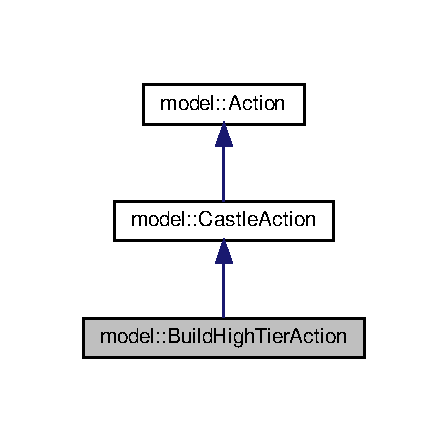
\includegraphics[width=215pt]{classmodel_1_1BuildHighTierAction__inherit__graph}
\end{center}
\end{figure}


Diagram współpracy dla model\+:\+:Build\+High\+Tier\+Action\+:\nopagebreak
\begin{figure}[H]
\begin{center}
\leavevmode
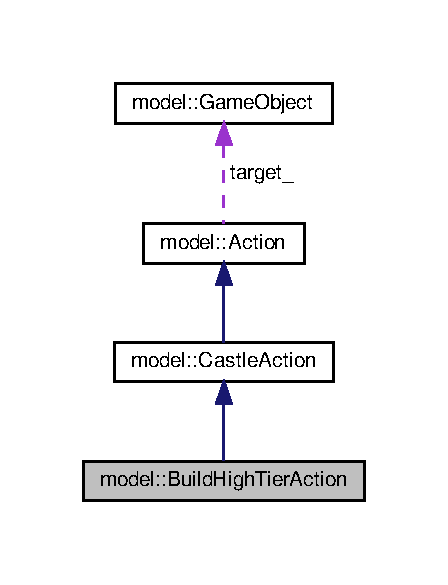
\includegraphics[width=215pt]{classmodel_1_1BuildHighTierAction__coll__graph}
\end{center}
\end{figure}
\subsection*{Metody publiczne}
\begin{DoxyCompactItemize}
\item 
\hyperlink{classmodel_1_1BuildHighTierAction_ae5b303402353343b947efba4ef9cd62d}{Build\+High\+Tier\+Action} (const \hyperlink{classmodel_1_1GameObject}{Game\+Object} \&target)
\begin{DoxyCompactList}\small\item\em Publiczny konstruktor z parametrem klasy \hyperlink{classmodel_1_1GameObject}{Game\+Object}. \end{DoxyCompactList}\item 
virtual void \hyperlink{classmodel_1_1BuildHighTierAction_a587f7c8efb015bbc00cb706e7e289edf}{print} ()
\begin{DoxyCompactList}\small\item\em Wirtualna metoda print. \end{DoxyCompactList}\end{DoxyCompactItemize}
\subsection*{Dodatkowe Dziedziczone Składowe}


\subsection{Opis szczegółowy}
Klasa \hyperlink{classmodel_1_1BuildHighTierAction}{Build\+High\+Tier\+Action}. 

Klasa imitująca klasę akcji budowy budynku wysokiego poziomu wydanego przez algorytm bota. 

\subsection{Dokumentacja konstruktora i destruktora}
\mbox{\Hypertarget{classmodel_1_1BuildHighTierAction_ae5b303402353343b947efba4ef9cd62d}\label{classmodel_1_1BuildHighTierAction_ae5b303402353343b947efba4ef9cd62d}} 
\index{model\+::\+Build\+High\+Tier\+Action@{model\+::\+Build\+High\+Tier\+Action}!Build\+High\+Tier\+Action@{Build\+High\+Tier\+Action}}
\index{Build\+High\+Tier\+Action@{Build\+High\+Tier\+Action}!model\+::\+Build\+High\+Tier\+Action@{model\+::\+Build\+High\+Tier\+Action}}
\subsubsection{\texorpdfstring{Build\+High\+Tier\+Action()}{BuildHighTierAction()}}
{\footnotesize\ttfamily model\+::\+Build\+High\+Tier\+Action\+::\+Build\+High\+Tier\+Action (\begin{DoxyParamCaption}\item[{const \hyperlink{classmodel_1_1GameObject}{Game\+Object} \&}]{target }\end{DoxyParamCaption})\hspace{0.3cm}{\ttfamily [inline]}}



Publiczny konstruktor z parametrem klasy \hyperlink{classmodel_1_1GameObject}{Game\+Object}. 


\begin{DoxyParams}{Parametry}
{\em target} & stała referencja na obiekt klasy \hyperlink{classmodel_1_1GameObject}{Game\+Object}. \\
\hline
\end{DoxyParams}


\subsection{Dokumentacja funkcji składowych}
\mbox{\Hypertarget{classmodel_1_1BuildHighTierAction_a587f7c8efb015bbc00cb706e7e289edf}\label{classmodel_1_1BuildHighTierAction_a587f7c8efb015bbc00cb706e7e289edf}} 
\index{model\+::\+Build\+High\+Tier\+Action@{model\+::\+Build\+High\+Tier\+Action}!print@{print}}
\index{print@{print}!model\+::\+Build\+High\+Tier\+Action@{model\+::\+Build\+High\+Tier\+Action}}
\subsubsection{\texorpdfstring{print()}{print()}}
{\footnotesize\ttfamily virtual void model\+::\+Build\+High\+Tier\+Action\+::print (\begin{DoxyParamCaption}{ }\end{DoxyParamCaption})\hspace{0.3cm}{\ttfamily [inline]}, {\ttfamily [virtual]}}



Wirtualna metoda print. 

Stosowana jedynie do informacji o zawartości kontenera decyzji 

Reimplementowana z \hyperlink{classmodel_1_1Action_a2955dbb4a69e38a48aa07d730fe2d77c}{model\+::\+Action}.



Dokumentacja dla tej klasy została wygenerowana z pliku\+:\begin{DoxyCompactItemize}
\item 
/home/bartlomiej/eclipse-\/workspace/lab\+\_\+3/src/bot/model/\hyperlink{build__high__tier__action_8hpp}{build\+\_\+high\+\_\+tier\+\_\+action.\+hpp}\end{DoxyCompactItemize}

\hypertarget{classmodel_1_1Building}{}\section{Dokumentacja klasy model\+:\+:Building}
\label{classmodel_1_1Building}\index{model\+::\+Building@{model\+::\+Building}}


Klasa \hyperlink{classmodel_1_1Building}{Building}.  




{\ttfamily \#include $<$building.\+hpp$>$}



Diagram dziedziczenia dla model\+:\+:Building\nopagebreak
\begin{figure}[H]
\begin{center}
\leavevmode
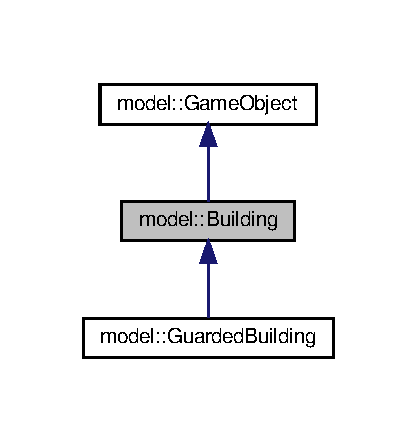
\includegraphics[width=200pt]{classmodel_1_1Building__inherit__graph}
\end{center}
\end{figure}


Diagram współpracy dla model\+:\+:Building\+:\nopagebreak
\begin{figure}[H]
\begin{center}
\leavevmode
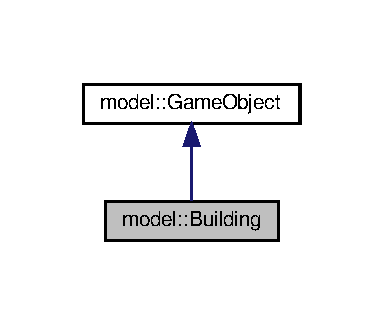
\includegraphics[width=184pt]{classmodel_1_1Building__coll__graph}
\end{center}
\end{figure}
\subsection*{Metody publiczne}
\begin{DoxyCompactItemize}
\item 
\hyperlink{classmodel_1_1Building_a17a7270e4283374db400aff509e59f27}{Building} (\hyperlink{tier_8hpp_a50a003ab1ea342f138c038fabfd1ee55}{Tier} tier, \hyperlink{status_8hpp_a822822ece62ee330ee656034849df887}{Status} status, int x, int y)
\begin{DoxyCompactList}\small\item\em Publiczny konstruktor. \end{DoxyCompactList}\item 
\hyperlink{classmodel_1_1Building_af8f2ee9d61a38ca85c6d035b8a1090e7}{Building} (int tier=0, int status=0, int x=0, int y=0)
\begin{DoxyCompactList}\small\item\em Publiczny konstruktor domyślny z parametrami integerowymi, konwertujący tier i status do enumeracji. \end{DoxyCompactList}\item 
\mbox{\Hypertarget{classmodel_1_1Building_a1926969cec3c46b9a38bf8a0c425dbc7}\label{classmodel_1_1Building_a1926969cec3c46b9a38bf8a0c425dbc7}} 
void \hyperlink{classmodel_1_1Building_a1926969cec3c46b9a38bf8a0c425dbc7}{take\+\_\+control} ()
\begin{DoxyCompactList}\small\item\em Funkcja objęcia kontroli; zmienia status budynku na przyjazny. \end{DoxyCompactList}\item 
\mbox{\Hypertarget{classmodel_1_1Building_a41dc923964b54592825864183d181964}\label{classmodel_1_1Building_a41dc923964b54592825864183d181964}} 
void \hyperlink{classmodel_1_1Building_a41dc923964b54592825864183d181964}{set\+\_\+status} (\hyperlink{status_8hpp_a822822ece62ee330ee656034849df887}{Status} status)
\begin{DoxyCompactList}\small\item\em Setter ustatwia status. \end{DoxyCompactList}\item 
\mbox{\Hypertarget{classmodel_1_1Building_a1fec2540ae9c9acf26734fcc2d8902d8}\label{classmodel_1_1Building_a1fec2540ae9c9acf26734fcc2d8902d8}} 
void \hyperlink{classmodel_1_1Building_a1fec2540ae9c9acf26734fcc2d8902d8}{set\+\_\+tier} (\hyperlink{tier_8hpp_a50a003ab1ea342f138c038fabfd1ee55}{Tier} tier)
\begin{DoxyCompactList}\small\item\em Setter ustawia poziom. \end{DoxyCompactList}\item 
\mbox{\Hypertarget{classmodel_1_1Building_a936de4be97a21d6b94fd5cddaab65ada}\label{classmodel_1_1Building_a936de4be97a21d6b94fd5cddaab65ada}} 
\hyperlink{tier_8hpp_a50a003ab1ea342f138c038fabfd1ee55}{Tier} \hyperlink{classmodel_1_1Building_a936de4be97a21d6b94fd5cddaab65ada}{get\+\_\+tier} () const
\begin{DoxyCompactList}\small\item\em Getter zwraca poziom. \end{DoxyCompactList}\item 
\mbox{\Hypertarget{classmodel_1_1Building_afd19261eed95d8568da5134ac62b9e1f}\label{classmodel_1_1Building_afd19261eed95d8568da5134ac62b9e1f}} 
\hyperlink{status_8hpp_a822822ece62ee330ee656034849df887}{Status} \hyperlink{classmodel_1_1Building_afd19261eed95d8568da5134ac62b9e1f}{get\+\_\+status} () const
\begin{DoxyCompactList}\small\item\em Getter zwraca status. \end{DoxyCompactList}\end{DoxyCompactItemize}


\subsection{Opis szczegółowy}
Klasa \hyperlink{classmodel_1_1Building}{Building}. 

Klasa budynku w rozumieniu bota, będąca obiektem gry, więc publicznie dziedzicząca po klasie \hyperlink{classmodel_1_1GameObject}{Game\+Object}. 

\subsection{Dokumentacja konstruktora i destruktora}
\mbox{\Hypertarget{classmodel_1_1Building_a17a7270e4283374db400aff509e59f27}\label{classmodel_1_1Building_a17a7270e4283374db400aff509e59f27}} 
\index{model\+::\+Building@{model\+::\+Building}!Building@{Building}}
\index{Building@{Building}!model\+::\+Building@{model\+::\+Building}}
\subsubsection{\texorpdfstring{Building()}{Building()}\hspace{0.1cm}{\footnotesize\ttfamily [1/2]}}
{\footnotesize\ttfamily model\+::\+Building\+::\+Building (\begin{DoxyParamCaption}\item[{\hyperlink{tier_8hpp_a50a003ab1ea342f138c038fabfd1ee55}{Tier}}]{tier,  }\item[{\hyperlink{status_8hpp_a822822ece62ee330ee656034849df887}{Status}}]{status,  }\item[{int}]{x,  }\item[{int}]{y }\end{DoxyParamCaption})\hspace{0.3cm}{\ttfamily [inline]}}



Publiczny konstruktor. 


\begin{DoxyParams}{Parametry}
{\em tier} & poziom budynku. \\
\hline
{\em status} & status budynku. \\
\hline
{\em x} & współrzędna x. \\
\hline
{\em y} & współrzędna y. \\
\hline
\end{DoxyParams}
\mbox{\Hypertarget{classmodel_1_1Building_af8f2ee9d61a38ca85c6d035b8a1090e7}\label{classmodel_1_1Building_af8f2ee9d61a38ca85c6d035b8a1090e7}} 
\index{model\+::\+Building@{model\+::\+Building}!Building@{Building}}
\index{Building@{Building}!model\+::\+Building@{model\+::\+Building}}
\subsubsection{\texorpdfstring{Building()}{Building()}\hspace{0.1cm}{\footnotesize\ttfamily [2/2]}}
{\footnotesize\ttfamily model\+::\+Building\+::\+Building (\begin{DoxyParamCaption}\item[{int}]{tier = {\ttfamily 0},  }\item[{int}]{status = {\ttfamily 0},  }\item[{int}]{x = {\ttfamily 0},  }\item[{int}]{y = {\ttfamily 0} }\end{DoxyParamCaption})\hspace{0.3cm}{\ttfamily [inline]}}



Publiczny konstruktor domyślny z parametrami integerowymi, konwertujący tier i status do enumeracji. 


\begin{DoxyParams}{Parametry}
{\em tier} & poziom budynku. \\
\hline
{\em status} & status budynku. \\
\hline
{\em x} & współrzędna x. \\
\hline
{\em y} & współrzędna y. \\
\hline
\end{DoxyParams}


Dokumentacja dla tej klasy została wygenerowana z pliku\+:\begin{DoxyCompactItemize}
\item 
/home/bartlomiej/eclipse-\/workspace/lab\+\_\+3/src/bot/model/\hyperlink{building_8hpp}{building.\+hpp}\end{DoxyCompactItemize}

\hypertarget{classmodel_1_1BuildLowTierAction}{}\section{Dokumentacja klasy model\+:\+:Build\+Low\+Tier\+Action}
\label{classmodel_1_1BuildLowTierAction}\index{model\+::\+Build\+Low\+Tier\+Action@{model\+::\+Build\+Low\+Tier\+Action}}


Klasa \hyperlink{classmodel_1_1BuildLowTierAction}{Build\+Low\+Tier\+Action}.  




{\ttfamily \#include $<$build\+\_\+low\+\_\+tier\+\_\+action.\+hpp$>$}



Diagram dziedziczenia dla model\+:\+:Build\+Low\+Tier\+Action\nopagebreak
\begin{figure}[H]
\begin{center}
\leavevmode
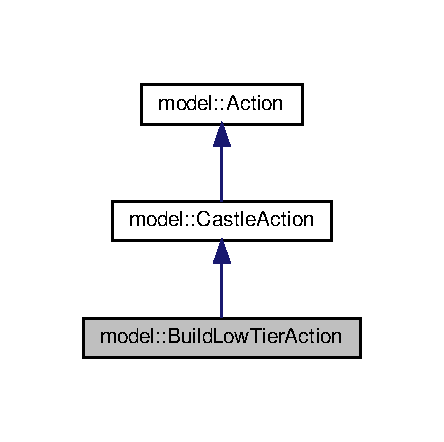
\includegraphics[width=213pt]{classmodel_1_1BuildLowTierAction__inherit__graph}
\end{center}
\end{figure}


Diagram współpracy dla model\+:\+:Build\+Low\+Tier\+Action\+:\nopagebreak
\begin{figure}[H]
\begin{center}
\leavevmode
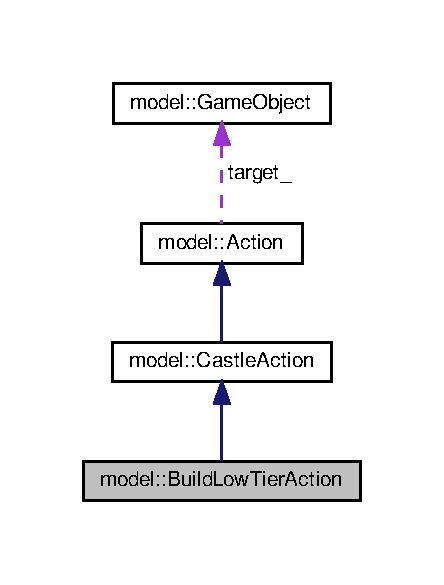
\includegraphics[width=213pt]{classmodel_1_1BuildLowTierAction__coll__graph}
\end{center}
\end{figure}
\subsection*{Metody publiczne}
\begin{DoxyCompactItemize}
\item 
\hyperlink{classmodel_1_1BuildLowTierAction_ad2f9e823c6e3d955590f0326f2ced54d}{Build\+Low\+Tier\+Action} (const \hyperlink{classmodel_1_1GameObject}{Game\+Object} \&target)
\begin{DoxyCompactList}\small\item\em Publiczny konstruktor z parametrem klasy \hyperlink{classmodel_1_1GameObject}{Game\+Object}. \end{DoxyCompactList}\item 
virtual void \hyperlink{classmodel_1_1BuildLowTierAction_a0917c29053656d5914125a30bcd51cce}{print} ()
\begin{DoxyCompactList}\small\item\em Wirtualna metoda print. \end{DoxyCompactList}\end{DoxyCompactItemize}
\subsection*{Dodatkowe Dziedziczone Składowe}


\subsection{Opis szczegółowy}
Klasa \hyperlink{classmodel_1_1BuildLowTierAction}{Build\+Low\+Tier\+Action}. 

Klasa imitująca klasę akcji budowy budynku niskiego poziomu wydanego przez algorytm bota. 

\subsection{Dokumentacja konstruktora i destruktora}
\mbox{\Hypertarget{classmodel_1_1BuildLowTierAction_ad2f9e823c6e3d955590f0326f2ced54d}\label{classmodel_1_1BuildLowTierAction_ad2f9e823c6e3d955590f0326f2ced54d}} 
\index{model\+::\+Build\+Low\+Tier\+Action@{model\+::\+Build\+Low\+Tier\+Action}!Build\+Low\+Tier\+Action@{Build\+Low\+Tier\+Action}}
\index{Build\+Low\+Tier\+Action@{Build\+Low\+Tier\+Action}!model\+::\+Build\+Low\+Tier\+Action@{model\+::\+Build\+Low\+Tier\+Action}}
\subsubsection{\texorpdfstring{Build\+Low\+Tier\+Action()}{BuildLowTierAction()}}
{\footnotesize\ttfamily model\+::\+Build\+Low\+Tier\+Action\+::\+Build\+Low\+Tier\+Action (\begin{DoxyParamCaption}\item[{const \hyperlink{classmodel_1_1GameObject}{Game\+Object} \&}]{target }\end{DoxyParamCaption})\hspace{0.3cm}{\ttfamily [inline]}}



Publiczny konstruktor z parametrem klasy \hyperlink{classmodel_1_1GameObject}{Game\+Object}. 


\begin{DoxyParams}{Parametry}
{\em target} & stała referencja na obiekt klasy \hyperlink{classmodel_1_1GameObject}{Game\+Object}. \\
\hline
\end{DoxyParams}


\subsection{Dokumentacja funkcji składowych}
\mbox{\Hypertarget{classmodel_1_1BuildLowTierAction_a0917c29053656d5914125a30bcd51cce}\label{classmodel_1_1BuildLowTierAction_a0917c29053656d5914125a30bcd51cce}} 
\index{model\+::\+Build\+Low\+Tier\+Action@{model\+::\+Build\+Low\+Tier\+Action}!print@{print}}
\index{print@{print}!model\+::\+Build\+Low\+Tier\+Action@{model\+::\+Build\+Low\+Tier\+Action}}
\subsubsection{\texorpdfstring{print()}{print()}}
{\footnotesize\ttfamily virtual void model\+::\+Build\+Low\+Tier\+Action\+::print (\begin{DoxyParamCaption}{ }\end{DoxyParamCaption})\hspace{0.3cm}{\ttfamily [inline]}, {\ttfamily [virtual]}}



Wirtualna metoda print. 

Stosowana jedynie do informacji o zawartości kontenera decyzji 

Reimplementowana z \hyperlink{classmodel_1_1Action_a2955dbb4a69e38a48aa07d730fe2d77c}{model\+::\+Action}.



Dokumentacja dla tej klasy została wygenerowana z pliku\+:\begin{DoxyCompactItemize}
\item 
/home/bartlomiej/eclipse-\/workspace/lab\+\_\+3/src/bot/model/\hyperlink{build__low__tier__action_8hpp}{build\+\_\+low\+\_\+tier\+\_\+action.\+hpp}\end{DoxyCompactItemize}

\hypertarget{classmodel_1_1BuildMidTierAction}{}\section{Dokumentacja klasy model\+:\+:Build\+Mid\+Tier\+Action}
\label{classmodel_1_1BuildMidTierAction}\index{model\+::\+Build\+Mid\+Tier\+Action@{model\+::\+Build\+Mid\+Tier\+Action}}


Klasa \hyperlink{classmodel_1_1BuildMidTierAction}{Build\+Mid\+Tier\+Action}.  




{\ttfamily \#include $<$build\+\_\+mid\+\_\+tier\+\_\+action.\+hpp$>$}



Diagram dziedziczenia dla model\+:\+:Build\+Mid\+Tier\+Action\nopagebreak
\begin{figure}[H]
\begin{center}
\leavevmode
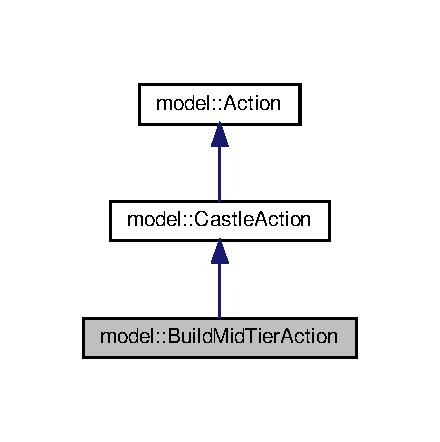
\includegraphics[width=211pt]{classmodel_1_1BuildMidTierAction__inherit__graph}
\end{center}
\end{figure}


Diagram współpracy dla model\+:\+:Build\+Mid\+Tier\+Action\+:\nopagebreak
\begin{figure}[H]
\begin{center}
\leavevmode
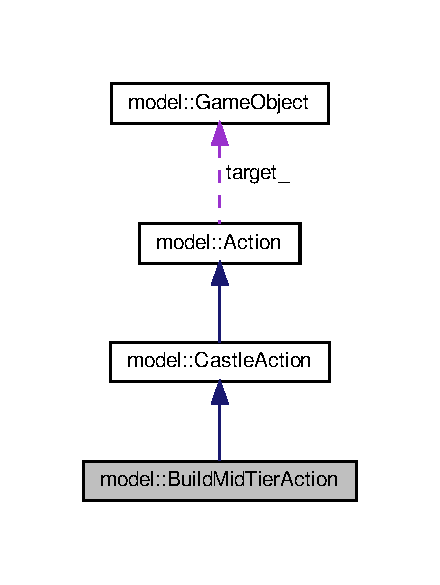
\includegraphics[width=211pt]{classmodel_1_1BuildMidTierAction__coll__graph}
\end{center}
\end{figure}
\subsection*{Metody publiczne}
\begin{DoxyCompactItemize}
\item 
\hyperlink{classmodel_1_1BuildMidTierAction_a8847e6f9fb9970ad1afaf2533147ed32}{Build\+Mid\+Tier\+Action} (const \hyperlink{classmodel_1_1GameObject}{Game\+Object} \&target)
\begin{DoxyCompactList}\small\item\em Publiczny konstruktor z parametrem klasy \hyperlink{classmodel_1_1GameObject}{Game\+Object}. \end{DoxyCompactList}\item 
virtual void \hyperlink{classmodel_1_1BuildMidTierAction_abec06b6ae68325996228e9b36c9d05d3}{print} ()
\begin{DoxyCompactList}\small\item\em Wirtualna metoda print. \end{DoxyCompactList}\end{DoxyCompactItemize}
\subsection*{Dodatkowe Dziedziczone Składowe}


\subsection{Opis szczegółowy}
Klasa \hyperlink{classmodel_1_1BuildMidTierAction}{Build\+Mid\+Tier\+Action}. 

Klasa imitująca klasę akcji budowy budynku średniego poziomu wydanego przez algorytm bota. 

\subsection{Dokumentacja konstruktora i destruktora}
\mbox{\Hypertarget{classmodel_1_1BuildMidTierAction_a8847e6f9fb9970ad1afaf2533147ed32}\label{classmodel_1_1BuildMidTierAction_a8847e6f9fb9970ad1afaf2533147ed32}} 
\index{model\+::\+Build\+Mid\+Tier\+Action@{model\+::\+Build\+Mid\+Tier\+Action}!Build\+Mid\+Tier\+Action@{Build\+Mid\+Tier\+Action}}
\index{Build\+Mid\+Tier\+Action@{Build\+Mid\+Tier\+Action}!model\+::\+Build\+Mid\+Tier\+Action@{model\+::\+Build\+Mid\+Tier\+Action}}
\subsubsection{\texorpdfstring{Build\+Mid\+Tier\+Action()}{BuildMidTierAction()}}
{\footnotesize\ttfamily model\+::\+Build\+Mid\+Tier\+Action\+::\+Build\+Mid\+Tier\+Action (\begin{DoxyParamCaption}\item[{const \hyperlink{classmodel_1_1GameObject}{Game\+Object} \&}]{target }\end{DoxyParamCaption})\hspace{0.3cm}{\ttfamily [inline]}}



Publiczny konstruktor z parametrem klasy \hyperlink{classmodel_1_1GameObject}{Game\+Object}. 


\begin{DoxyParams}{Parametry}
{\em target} & stała referencja na obiekt klasy \hyperlink{classmodel_1_1GameObject}{Game\+Object}. \\
\hline
\end{DoxyParams}


\subsection{Dokumentacja funkcji składowych}
\mbox{\Hypertarget{classmodel_1_1BuildMidTierAction_abec06b6ae68325996228e9b36c9d05d3}\label{classmodel_1_1BuildMidTierAction_abec06b6ae68325996228e9b36c9d05d3}} 
\index{model\+::\+Build\+Mid\+Tier\+Action@{model\+::\+Build\+Mid\+Tier\+Action}!print@{print}}
\index{print@{print}!model\+::\+Build\+Mid\+Tier\+Action@{model\+::\+Build\+Mid\+Tier\+Action}}
\subsubsection{\texorpdfstring{print()}{print()}}
{\footnotesize\ttfamily virtual void model\+::\+Build\+Mid\+Tier\+Action\+::print (\begin{DoxyParamCaption}{ }\end{DoxyParamCaption})\hspace{0.3cm}{\ttfamily [inline]}, {\ttfamily [virtual]}}



Wirtualna metoda print. 

Stosowana jedynie do informacji o zawartości kontenera decyzji 

Reimplementowana z \hyperlink{classmodel_1_1Action_a2955dbb4a69e38a48aa07d730fe2d77c}{model\+::\+Action}.



Dokumentacja dla tej klasy została wygenerowana z pliku\+:\begin{DoxyCompactItemize}
\item 
/home/bartlomiej/eclipse-\/workspace/lab\+\_\+3/src/bot/model/\hyperlink{build__mid__tier__action_8hpp}{build\+\_\+mid\+\_\+tier\+\_\+action.\+hpp}\end{DoxyCompactItemize}

\hypertarget{classmodel_1_1Castle}{}\section{Dokumentacja klasy model\+:\+:Castle}
\label{classmodel_1_1Castle}\index{model\+::\+Castle@{model\+::\+Castle}}


Klasa \hyperlink{classmodel_1_1Castle}{Castle}.  




{\ttfamily \#include $<$castle.\+hpp$>$}



Diagram dziedziczenia dla model\+:\+:Castle\nopagebreak
\begin{figure}[H]
\begin{center}
\leavevmode
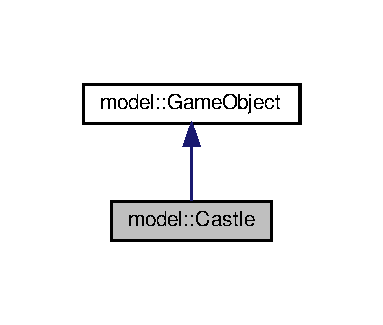
\includegraphics[width=184pt]{classmodel_1_1Castle__inherit__graph}
\end{center}
\end{figure}


Diagram współpracy dla model\+:\+:Castle\+:\nopagebreak
\begin{figure}[H]
\begin{center}
\leavevmode
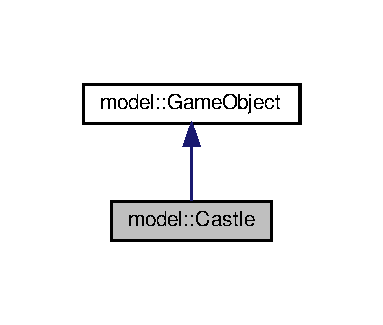
\includegraphics[width=184pt]{classmodel_1_1Castle__coll__graph}
\end{center}
\end{figure}
\subsection*{Metody publiczne}
\begin{DoxyCompactItemize}
\item 
\hyperlink{classmodel_1_1Castle_a26e1b6313f73e34d1babd517f5d56c1f}{Castle} (int high\+\_\+tier\+\_\+army\+\_\+num=0, int mid\+\_\+tier\+\_\+army\+\_\+num=0, int low\+\_\+tier\+\_\+army\+\_\+num=0, \hyperlink{status_8hpp_a822822ece62ee330ee656034849df887}{Status} status=Status\+::\+N\+E\+U\+T\+R\+AL, int high\+\_\+tier\+\_\+buildings\+\_\+num=0, int mid\+\_\+tier\+\_\+buildings\+\_\+num=0, int low\+\_\+tier\+\_\+buildings\+\_\+num=0, int high\+\_\+tier\+\_\+recruitment\+\_\+num=0, int mid\+\_\+tier\+\_\+recruitment\+\_\+num=0, int low\+\_\+tier\+\_\+recruitment\+\_\+num=0, int x=0, int y=0)
\begin{DoxyCompactList}\small\item\em Publiczny konstruktor domyślny. \end{DoxyCompactList}\item 
\hyperlink{classmodel_1_1Castle_af4e3122af95b49521d4b57d7ec671712}{Castle} (const std\+::vector$<$ int $>$ \&params, \hyperlink{status_8hpp_a822822ece62ee330ee656034849df887}{Status} status)
\begin{DoxyCompactList}\small\item\em Publiczny konstruktor. \end{DoxyCompactList}\item 
\mbox{\Hypertarget{classmodel_1_1Castle_a3ee46a8f9e30c7e1ff7bef9d650c233e}\label{classmodel_1_1Castle_a3ee46a8f9e30c7e1ff7bef9d650c233e}} 
double \hyperlink{classmodel_1_1Castle_a3ee46a8f9e30c7e1ff7bef9d650c233e}{defence\+\_\+bonus} () const
\begin{DoxyCompactList}\small\item\em Funkcja obliczająca bonus obronny. \end{DoxyCompactList}\item 
\mbox{\Hypertarget{classmodel_1_1Castle_a668531c7d4699e36dc7f1f4d449653dc}\label{classmodel_1_1Castle_a668531c7d4699e36dc7f1f4d449653dc}} 
void \hyperlink{classmodel_1_1Castle_a668531c7d4699e36dc7f1f4d449653dc}{build\+\_\+low\+\_\+tier} ()
\begin{DoxyCompactList}\small\item\em Funkcja budowania budynku niskiego poziomu; zwiększa liczbę tych budynków w zamku. \end{DoxyCompactList}\item 
\mbox{\Hypertarget{classmodel_1_1Castle_a59e4a67ca637be7f4624915e514e761f}\label{classmodel_1_1Castle_a59e4a67ca637be7f4624915e514e761f}} 
void \hyperlink{classmodel_1_1Castle_a59e4a67ca637be7f4624915e514e761f}{build\+\_\+mid\+\_\+tier} ()
\begin{DoxyCompactList}\small\item\em Funkcja budowania budynku średniego poziomu; zwiększa liczbę tych budynków w zamku. \end{DoxyCompactList}\item 
\mbox{\Hypertarget{classmodel_1_1Castle_a89497c4fa84a2264329d36683d5d15d1}\label{classmodel_1_1Castle_a89497c4fa84a2264329d36683d5d15d1}} 
void \hyperlink{classmodel_1_1Castle_a89497c4fa84a2264329d36683d5d15d1}{build\+\_\+high\+\_\+tier} ()
\begin{DoxyCompactList}\small\item\em Funkcja budowania budynku wysokiego poziomu; zwiększa liczbę tych budynków w zamku. \end{DoxyCompactList}\item 
\mbox{\Hypertarget{classmodel_1_1Castle_a35900af063f73ccb135e66796c48e383}\label{classmodel_1_1Castle_a35900af063f73ccb135e66796c48e383}} 
void \hyperlink{classmodel_1_1Castle_a35900af063f73ccb135e66796c48e383}{recruit\+\_\+high\+\_\+tier} (int quantity)
\begin{DoxyCompactList}\small\item\em Funkcja rekrutowania jednostki wysokiego poziomu; zmniejsza liczbę możliwych do rektutacji i zwiększa liczbę jednostek w garnizonie. \end{DoxyCompactList}\item 
\mbox{\Hypertarget{classmodel_1_1Castle_a8b8a25ca83a7c8d935bc3892109abe6f}\label{classmodel_1_1Castle_a8b8a25ca83a7c8d935bc3892109abe6f}} 
void \hyperlink{classmodel_1_1Castle_a8b8a25ca83a7c8d935bc3892109abe6f}{recruit\+\_\+mid\+\_\+tier} (int quantity)
\begin{DoxyCompactList}\small\item\em Funkcja rekrutowania jednostki średniego poziomu; zmniejsza liczbę możliwych do rektutacji i zwiększa liczbę jednostek w garnizonie. \end{DoxyCompactList}\item 
\mbox{\Hypertarget{classmodel_1_1Castle_aa80ab7329c7db0de69ecfa1ab4ed8e17}\label{classmodel_1_1Castle_aa80ab7329c7db0de69ecfa1ab4ed8e17}} 
void \hyperlink{classmodel_1_1Castle_aa80ab7329c7db0de69ecfa1ab4ed8e17}{recruit\+\_\+low\+\_\+tier} (int quantity)
\begin{DoxyCompactList}\small\item\em Funkcja rekrutowania jednostki niskiego poziomu; zmniejsza liczbę możliwych do rektutacji i zwiększa liczbę jednostek w garnizonie. \end{DoxyCompactList}\item 
\mbox{\Hypertarget{classmodel_1_1Castle_abc66c3c106ba785d61a8c18c747105fb}\label{classmodel_1_1Castle_abc66c3c106ba785d61a8c18c747105fb}} 
int \hyperlink{classmodel_1_1Castle_abc66c3c106ba785d61a8c18c747105fb}{get\+\_\+high\+\_\+tier\+\_\+recruitment\+\_\+num} () const
\begin{DoxyCompactList}\small\item\em Getter zwraca liczbę jednostek wysokiego poziomu możliwą do rekrutacji. \end{DoxyCompactList}\item 
\mbox{\Hypertarget{classmodel_1_1Castle_a8d51d7365175bf1969f66115f22f5f6c}\label{classmodel_1_1Castle_a8d51d7365175bf1969f66115f22f5f6c}} 
int \hyperlink{classmodel_1_1Castle_a8d51d7365175bf1969f66115f22f5f6c}{get\+\_\+mid\+\_\+tier\+\_\+recruitment\+\_\+num} () const
\begin{DoxyCompactList}\small\item\em Getter zwraca liczbę jednostek średniego poziomu możliwą do rekrutacji. \end{DoxyCompactList}\item 
\mbox{\Hypertarget{classmodel_1_1Castle_aeeb01c7a4afe8ebfd383120fe9788fce}\label{classmodel_1_1Castle_aeeb01c7a4afe8ebfd383120fe9788fce}} 
int \hyperlink{classmodel_1_1Castle_aeeb01c7a4afe8ebfd383120fe9788fce}{get\+\_\+low\+\_\+tier\+\_\+recruitment\+\_\+num} () const
\begin{DoxyCompactList}\small\item\em Getter zwraca liczbę jednostek niskiego poziomu możliwą do rekrutacji. \end{DoxyCompactList}\item 
\mbox{\Hypertarget{classmodel_1_1Castle_afa5847ea8e097aaa3bfeb4f040514225}\label{classmodel_1_1Castle_afa5847ea8e097aaa3bfeb4f040514225}} 
bool \hyperlink{classmodel_1_1Castle_afa5847ea8e097aaa3bfeb4f040514225}{is\+\_\+development\+\_\+available\+\_\+high} () const
\begin{DoxyCompactList}\small\item\em Funkcja zwraca wartośc logiczą czy budowa budynku wysokiego poziomu jest możliwa. \end{DoxyCompactList}\item 
\mbox{\Hypertarget{classmodel_1_1Castle_a125b8044d0a31b72941d14bad9a279ea}\label{classmodel_1_1Castle_a125b8044d0a31b72941d14bad9a279ea}} 
bool \hyperlink{classmodel_1_1Castle_a125b8044d0a31b72941d14bad9a279ea}{is\+\_\+development\+\_\+available\+\_\+mid} () const
\begin{DoxyCompactList}\small\item\em Funkcja zwraca wartośc logiczą czy budowa budynku średniego poziomu jest możliwa. \end{DoxyCompactList}\item 
\mbox{\Hypertarget{classmodel_1_1Castle_a58687978e87a7a83d20093f250e04ad7}\label{classmodel_1_1Castle_a58687978e87a7a83d20093f250e04ad7}} 
bool \hyperlink{classmodel_1_1Castle_a58687978e87a7a83d20093f250e04ad7}{is\+\_\+development\+\_\+available\+\_\+low} () const
\begin{DoxyCompactList}\small\item\em Funkcja zwraca wartośc logiczą czy budowa budynku niskiego poziomu jest możliwa. \end{DoxyCompactList}\item 
\mbox{\Hypertarget{classmodel_1_1Castle_ab1755d63a55a286002ef49b631b00d76}\label{classmodel_1_1Castle_ab1755d63a55a286002ef49b631b00d76}} 
int \hyperlink{classmodel_1_1Castle_ab1755d63a55a286002ef49b631b00d76}{count\+\_\+castle\+\_\+force} () const
\begin{DoxyCompactList}\small\item\em Funkcja obliczająca siłę zamku; mnoży siłę garnizonu przez bonus obronny. \end{DoxyCompactList}\item 
\mbox{\Hypertarget{classmodel_1_1Castle_a3de598a4bb266b1d6d0920e0a53f7e35}\label{classmodel_1_1Castle_a3de598a4bb266b1d6d0920e0a53f7e35}} 
void \hyperlink{classmodel_1_1Castle_a3de598a4bb266b1d6d0920e0a53f7e35}{conquer} ()
\begin{DoxyCompactList}\small\item\em Funkcja zdobądź zamek; ustawia jego status na przyjazny i zeruje garnizon zamku. \end{DoxyCompactList}\item 
\mbox{\Hypertarget{classmodel_1_1Castle_a74b526c24b8ac302c625b9c1162c9d25}\label{classmodel_1_1Castle_a74b526c24b8ac302c625b9c1162c9d25}} 
\hyperlink{status_8hpp_a822822ece62ee330ee656034849df887}{Status} \hyperlink{classmodel_1_1Castle_a74b526c24b8ac302c625b9c1162c9d25}{get\+\_\+status} () const
\begin{DoxyCompactList}\small\item\em Getter zwraca status zamku. \end{DoxyCompactList}\end{DoxyCompactItemize}
\subsection*{Statyczne atrybuty publiczne}
\begin{DoxyCompactItemize}
\item 
\mbox{\Hypertarget{classmodel_1_1Castle_a33917ec4ec233ca0155ef1bb1e6e71c3}\label{classmodel_1_1Castle_a33917ec4ec233ca0155ef1bb1e6e71c3}} 
static const int \hyperlink{classmodel_1_1Castle_a33917ec4ec233ca0155ef1bb1e6e71c3}{L\+O\+W\+\_\+\+T\+I\+E\+R\+\_\+\+B\+U\+I\+L\+D\+I\+N\+G\+\_\+\+C\+O\+ST} = 1000
\begin{DoxyCompactList}\small\item\em Statyczna stała; koszt wybudowania budynku niskiego poziomu. \end{DoxyCompactList}\item 
\mbox{\Hypertarget{classmodel_1_1Castle_a097c1b13b5b2963e40ad22c38fbc2702}\label{classmodel_1_1Castle_a097c1b13b5b2963e40ad22c38fbc2702}} 
static const int \hyperlink{classmodel_1_1Castle_a097c1b13b5b2963e40ad22c38fbc2702}{M\+I\+D\+\_\+\+T\+I\+E\+R\+\_\+\+B\+U\+I\+L\+D\+I\+N\+G\+\_\+\+C\+O\+ST} = 4000
\begin{DoxyCompactList}\small\item\em Statyczna stała; koszt wybudowania budynku średniego poziomu. \end{DoxyCompactList}\item 
\mbox{\Hypertarget{classmodel_1_1Castle_a35ec993e948dc5514f248beba9dcd27c}\label{classmodel_1_1Castle_a35ec993e948dc5514f248beba9dcd27c}} 
static const int \hyperlink{classmodel_1_1Castle_a35ec993e948dc5514f248beba9dcd27c}{H\+I\+G\+H\+\_\+\+T\+I\+E\+R\+\_\+\+B\+U\+I\+L\+D\+I\+N\+G\+\_\+\+C\+O\+ST} = 15000
\begin{DoxyCompactList}\small\item\em Statyczna stała; koszt wybudowania budynku wysokiego poziomu. \end{DoxyCompactList}\item 
\mbox{\Hypertarget{classmodel_1_1Castle_ac5c4d0b65b66c7058a87eecf4b712b78}\label{classmodel_1_1Castle_ac5c4d0b65b66c7058a87eecf4b712b78}} 
static const int \hyperlink{classmodel_1_1Castle_ac5c4d0b65b66c7058a87eecf4b712b78}{L\+O\+W\+\_\+\+T\+I\+E\+R\+\_\+\+E\+N\+T\+I\+T\+Y\+\_\+\+C\+O\+ST} = 100
\begin{DoxyCompactList}\small\item\em Statyczna stała; koszt rekrutacji jednostki niskiego poziomu. \end{DoxyCompactList}\item 
\mbox{\Hypertarget{classmodel_1_1Castle_acccacb70864e05f2c299abefa91df555}\label{classmodel_1_1Castle_acccacb70864e05f2c299abefa91df555}} 
static const int \hyperlink{classmodel_1_1Castle_acccacb70864e05f2c299abefa91df555}{M\+I\+D\+\_\+\+T\+I\+E\+R\+\_\+\+E\+N\+T\+I\+T\+Y\+\_\+\+C\+O\+ST} = 400
\begin{DoxyCompactList}\small\item\em Statyczna stała; koszt rekrutacji jednostki średniego poziomu. \end{DoxyCompactList}\item 
\mbox{\Hypertarget{classmodel_1_1Castle_ac14c39feb4b10c1b5e03db76f26cabd2}\label{classmodel_1_1Castle_ac14c39feb4b10c1b5e03db76f26cabd2}} 
static const int \hyperlink{classmodel_1_1Castle_ac14c39feb4b10c1b5e03db76f26cabd2}{H\+I\+G\+H\+\_\+\+T\+I\+E\+R\+\_\+\+E\+N\+T\+I\+T\+Y\+\_\+\+C\+O\+ST} = 2000
\begin{DoxyCompactList}\small\item\em Statyczna stała; koszt rekrutacji jednostki wysokiego poziomu. \end{DoxyCompactList}\item 
\mbox{\Hypertarget{classmodel_1_1Castle_a78afd159a8925f53cd895df7394dc1f2}\label{classmodel_1_1Castle_a78afd159a8925f53cd895df7394dc1f2}} 
static const int \hyperlink{classmodel_1_1Castle_a78afd159a8925f53cd895df7394dc1f2}{M\+A\+X\+\_\+\+H\+I\+G\+H\+\_\+\+T\+I\+E\+R\+\_\+\+B\+U\+I\+L\+D\+I\+N\+GS} = 3
\begin{DoxyCompactList}\small\item\em Statyczna stała; maksymalna liczba budynków wysokiego poziomu. \end{DoxyCompactList}\item 
\mbox{\Hypertarget{classmodel_1_1Castle_a343dfe0538d36cf80ab632f5f6221eb2}\label{classmodel_1_1Castle_a343dfe0538d36cf80ab632f5f6221eb2}} 
static const int \hyperlink{classmodel_1_1Castle_a343dfe0538d36cf80ab632f5f6221eb2}{M\+A\+X\+\_\+\+M\+I\+D\+\_\+\+T\+I\+E\+R\+\_\+\+B\+U\+I\+L\+D\+I\+N\+GS} = 5
\begin{DoxyCompactList}\small\item\em Statyczna stała; maksymalna liczba budynków średniego poziomu. \end{DoxyCompactList}\item 
\mbox{\Hypertarget{classmodel_1_1Castle_aff52e7e4d26f5062f1943a10a8b753d3}\label{classmodel_1_1Castle_aff52e7e4d26f5062f1943a10a8b753d3}} 
static const int \hyperlink{classmodel_1_1Castle_aff52e7e4d26f5062f1943a10a8b753d3}{M\+A\+X\+\_\+\+L\+O\+W\+\_\+\+T\+I\+E\+R\+\_\+\+B\+U\+I\+L\+D\+I\+N\+GS} = 10
\begin{DoxyCompactList}\small\item\em Statyczna stała; maksymalna liczba budynków niskiego poziomu. \end{DoxyCompactList}\item 
\mbox{\Hypertarget{classmodel_1_1Castle_a8aa1907d2863606d0aab8ae449dd7d57}\label{classmodel_1_1Castle_a8aa1907d2863606d0aab8ae449dd7d57}} 
static constexpr double \hyperlink{classmodel_1_1Castle_a8aa1907d2863606d0aab8ae449dd7d57}{L\+O\+W\+\_\+\+T\+I\+E\+R\+\_\+\+B\+U\+I\+L\+D\+I\+N\+G\+\_\+\+D\+E\+F\+E\+N\+C\+E\+\_\+\+B\+O\+N\+US} = 0.\+01
\begin{DoxyCompactList}\small\item\em Statyczna stała; bonus do obrony od budynku niskiego poziomu. \end{DoxyCompactList}\item 
\mbox{\Hypertarget{classmodel_1_1Castle_a26afa71c719e1009f3c0884e9064ae61}\label{classmodel_1_1Castle_a26afa71c719e1009f3c0884e9064ae61}} 
static constexpr double \hyperlink{classmodel_1_1Castle_a26afa71c719e1009f3c0884e9064ae61}{M\+I\+D\+\_\+\+T\+I\+E\+R\+\_\+\+B\+U\+I\+L\+D\+I\+N\+G\+\_\+\+D\+E\+F\+E\+N\+C\+E\+\_\+\+B\+O\+N\+US} = 0.\+02
\begin{DoxyCompactList}\small\item\em Statyczna stała; bonus do obrony od budynku średniego poziomu. \end{DoxyCompactList}\item 
\mbox{\Hypertarget{classmodel_1_1Castle_a64d14929c22abc58acbae97420111370}\label{classmodel_1_1Castle_a64d14929c22abc58acbae97420111370}} 
static constexpr double \hyperlink{classmodel_1_1Castle_a64d14929c22abc58acbae97420111370}{H\+I\+G\+H\+\_\+\+T\+I\+E\+R\+\_\+\+B\+U\+I\+L\+D\+I\+N\+G\+\_\+\+D\+E\+F\+E\+N\+C\+E\+\_\+\+B\+O\+N\+US} = 0.\+05
\begin{DoxyCompactList}\small\item\em Statyczna stała; bonus do obrony od budynku wysokiego poziomu. \end{DoxyCompactList}\end{DoxyCompactItemize}


\subsection{Opis szczegółowy}
Klasa \hyperlink{classmodel_1_1Castle}{Castle}. 

Klasa zamku w rozumieniu bota, będąca obiektem gry, więc publicznie dziedzicząca po klasie \hyperlink{classmodel_1_1GameObject}{Game\+Object}. 

\subsection{Dokumentacja konstruktora i destruktora}
\mbox{\Hypertarget{classmodel_1_1Castle_a26e1b6313f73e34d1babd517f5d56c1f}\label{classmodel_1_1Castle_a26e1b6313f73e34d1babd517f5d56c1f}} 
\index{model\+::\+Castle@{model\+::\+Castle}!Castle@{Castle}}
\index{Castle@{Castle}!model\+::\+Castle@{model\+::\+Castle}}
\subsubsection{\texorpdfstring{Castle()}{Castle()}\hspace{0.1cm}{\footnotesize\ttfamily [1/2]}}
{\footnotesize\ttfamily model\+::\+Castle\+::\+Castle (\begin{DoxyParamCaption}\item[{int}]{high\+\_\+tier\+\_\+army\+\_\+num = {\ttfamily 0},  }\item[{int}]{mid\+\_\+tier\+\_\+army\+\_\+num = {\ttfamily 0},  }\item[{int}]{low\+\_\+tier\+\_\+army\+\_\+num = {\ttfamily 0},  }\item[{\hyperlink{status_8hpp_a822822ece62ee330ee656034849df887}{Status}}]{status = {\ttfamily Status\+:\+:NEUTRAL},  }\item[{int}]{high\+\_\+tier\+\_\+buildings\+\_\+num = {\ttfamily 0},  }\item[{int}]{mid\+\_\+tier\+\_\+buildings\+\_\+num = {\ttfamily 0},  }\item[{int}]{low\+\_\+tier\+\_\+buildings\+\_\+num = {\ttfamily 0},  }\item[{int}]{high\+\_\+tier\+\_\+recruitment\+\_\+num = {\ttfamily 0},  }\item[{int}]{mid\+\_\+tier\+\_\+recruitment\+\_\+num = {\ttfamily 0},  }\item[{int}]{low\+\_\+tier\+\_\+recruitment\+\_\+num = {\ttfamily 0},  }\item[{int}]{x = {\ttfamily 0},  }\item[{int}]{y = {\ttfamily 0} }\end{DoxyParamCaption})\hspace{0.3cm}{\ttfamily [inline]}}



Publiczny konstruktor domyślny. 


\begin{DoxyParams}{Parametry}
{\em high\+\_\+tier\+\_\+army\+\_\+num} & liczba jednostek wysokiego poziomu w garnizonie. \\
\hline
{\em mid\+\_\+tier\+\_\+army\+\_\+num} & liczba jednostek średniego poziomu w garnizonie. \\
\hline
{\em low\+\_\+tier\+\_\+army\+\_\+num} & liczba jednostek niskiego poziomu w garnizonie. \\
\hline
{\em status} & status zamku. \\
\hline
{\em high\+\_\+tier\+\_\+buildings\+\_\+num} & liczba budynków wysokiego poziomu w zamku. \\
\hline
{\em mid\+\_\+tier\+\_\+buildings\+\_\+num} & liczba budynków średniego poziomu w zamku. \\
\hline
{\em low\+\_\+tier\+\_\+buildings\+\_\+num} & liczba budynków niskiego poziomu w zamku. \\
\hline
{\em high\+\_\+tier\+\_\+recruitment\+\_\+num} & liczba jednostek wysokiego poziomu możliwych do rekrutacji w zamku. \\
\hline
{\em mid\+\_\+tier\+\_\+recruitment\+\_\+num} & liczba jednostek średniego poziomu możliwych do rekrutacji w zamku. \\
\hline
{\em low\+\_\+tier\+\_\+recruitment\+\_\+num} & liczba jednostek niskiego poziomu możliwych do rekrutacji w zamku. \\
\hline
{\em x} & współrzędna x. \\
\hline
{\em y} & współrzędna y. \\
\hline
\end{DoxyParams}
\mbox{\Hypertarget{classmodel_1_1Castle_af4e3122af95b49521d4b57d7ec671712}\label{classmodel_1_1Castle_af4e3122af95b49521d4b57d7ec671712}} 
\index{model\+::\+Castle@{model\+::\+Castle}!Castle@{Castle}}
\index{Castle@{Castle}!model\+::\+Castle@{model\+::\+Castle}}
\subsubsection{\texorpdfstring{Castle()}{Castle()}\hspace{0.1cm}{\footnotesize\ttfamily [2/2]}}
{\footnotesize\ttfamily model\+::\+Castle\+::\+Castle (\begin{DoxyParamCaption}\item[{const std\+::vector$<$ int $>$ \&}]{params,  }\item[{\hyperlink{status_8hpp_a822822ece62ee330ee656034849df887}{Status}}]{status }\end{DoxyParamCaption})\hspace{0.3cm}{\ttfamily [inline]}}



Publiczny konstruktor. 


\begin{DoxyParams}{Parametry}
{\em params} & wektor parametrów integerowych. \\
\hline
{\em status} & status bohatera. \\
\hline
\end{DoxyParams}


Dokumentacja dla tej klasy została wygenerowana z pliku\+:\begin{DoxyCompactItemize}
\item 
/home/bartlomiej/eclipse-\/workspace/lab\+\_\+3/src/bot/model/\hyperlink{castle_8hpp}{castle.\+hpp}\end{DoxyCompactItemize}

\hypertarget{classmodel_1_1CastleAction}{}\section{Dokumentacja klasy model\+:\+:Castle\+Action}
\label{classmodel_1_1CastleAction}\index{model\+::\+Castle\+Action@{model\+::\+Castle\+Action}}


Klasa \hyperlink{classmodel_1_1CastleAction}{Castle\+Action}.  




{\ttfamily \#include $<$castle\+\_\+actions.\+hpp$>$}



Diagram dziedziczenia dla model\+:\+:Castle\+Action\nopagebreak
\begin{figure}[H]
\begin{center}
\leavevmode
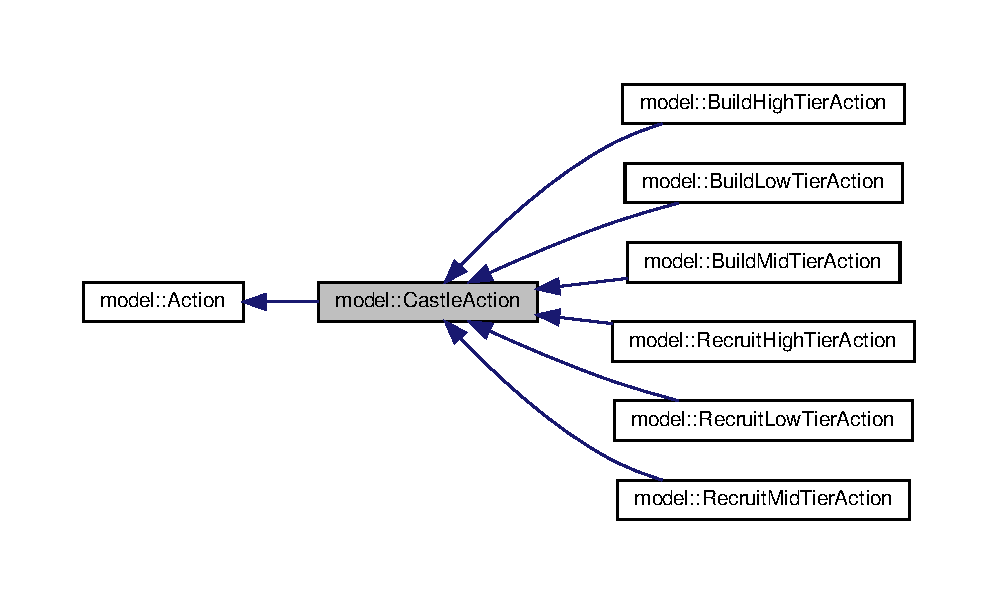
\includegraphics[width=350pt]{classmodel_1_1CastleAction__inherit__graph}
\end{center}
\end{figure}


Diagram współpracy dla model\+:\+:Castle\+Action\+:\nopagebreak
\begin{figure}[H]
\begin{center}
\leavevmode
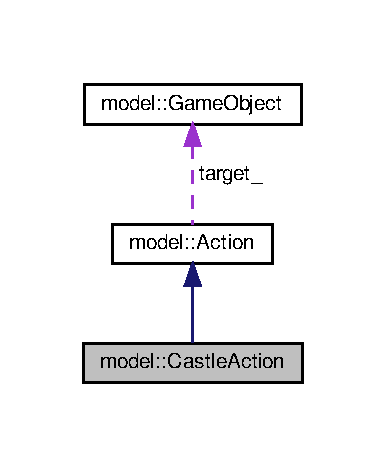
\includegraphics[width=185pt]{classmodel_1_1CastleAction__coll__graph}
\end{center}
\end{figure}
\subsection*{Metody publiczne}
\begin{DoxyCompactItemize}
\item 
\hyperlink{classmodel_1_1CastleAction_ab40d2d8ae98e800d3feb596296476e33}{Castle\+Action} (const \hyperlink{classmodel_1_1GameObject}{Game\+Object} \&target)
\begin{DoxyCompactList}\small\item\em Publiczny konstruktor z parametrem klasy \hyperlink{classmodel_1_1GameObject}{Game\+Object}. \end{DoxyCompactList}\item 
\mbox{\Hypertarget{classmodel_1_1CastleAction_a93842e1154b02939c422f143f20694d3}\label{classmodel_1_1CastleAction_a93842e1154b02939c422f143f20694d3}} 
virtual \hyperlink{classmodel_1_1CastleAction_a93842e1154b02939c422f143f20694d3}{$\sim$\+Castle\+Action} ()
\begin{DoxyCompactList}\small\item\em Wirtualny destruktor. \end{DoxyCompactList}\end{DoxyCompactItemize}
\subsection*{Dodatkowe Dziedziczone Składowe}


\subsection{Opis szczegółowy}
Klasa \hyperlink{classmodel_1_1CastleAction}{Castle\+Action}. 

Klasa bazowa dla akcji zamku wydanych przez algorytm bota. 

\subsection{Dokumentacja konstruktora i destruktora}
\mbox{\Hypertarget{classmodel_1_1CastleAction_ab40d2d8ae98e800d3feb596296476e33}\label{classmodel_1_1CastleAction_ab40d2d8ae98e800d3feb596296476e33}} 
\index{model\+::\+Castle\+Action@{model\+::\+Castle\+Action}!Castle\+Action@{Castle\+Action}}
\index{Castle\+Action@{Castle\+Action}!model\+::\+Castle\+Action@{model\+::\+Castle\+Action}}
\subsubsection{\texorpdfstring{Castle\+Action()}{CastleAction()}}
{\footnotesize\ttfamily model\+::\+Castle\+Action\+::\+Castle\+Action (\begin{DoxyParamCaption}\item[{const \hyperlink{classmodel_1_1GameObject}{Game\+Object} \&}]{target }\end{DoxyParamCaption})\hspace{0.3cm}{\ttfamily [inline]}, {\ttfamily [explicit]}}



Publiczny konstruktor z parametrem klasy \hyperlink{classmodel_1_1GameObject}{Game\+Object}. 


\begin{DoxyParams}{Parametry}
{\em target} & stała referencja na obiekt klasy \hyperlink{classmodel_1_1GameObject}{Game\+Object}. \\
\hline
\end{DoxyParams}


Dokumentacja dla tej klasy została wygenerowana z pliku\+:\begin{DoxyCompactItemize}
\item 
/home/bartlomiej/eclipse-\/workspace/lab\+\_\+3/src/bot/model/\hyperlink{castle__actions_8hpp}{castle\+\_\+actions.\+hpp}\end{DoxyCompactItemize}

\hypertarget{classmodel_1_1EnterAction}{}\section{Dokumentacja klasy model\+:\+:Enter\+Action}
\label{classmodel_1_1EnterAction}\index{model\+::\+Enter\+Action@{model\+::\+Enter\+Action}}


Klasa \hyperlink{classmodel_1_1EnterAction}{Enter\+Action}.  




{\ttfamily \#include $<$enter\+\_\+action.\+hpp$>$}



Diagram dziedziczenia dla model\+:\+:Enter\+Action\nopagebreak
\begin{figure}[H]
\begin{center}
\leavevmode
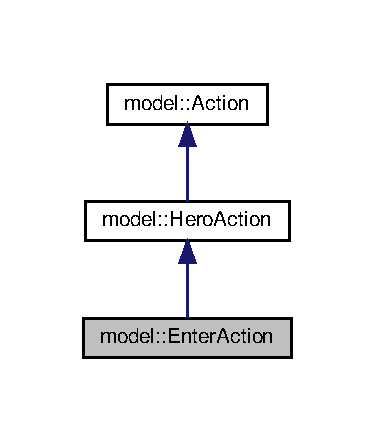
\includegraphics[width=180pt]{classmodel_1_1EnterAction__inherit__graph}
\end{center}
\end{figure}


Diagram współpracy dla model\+:\+:Enter\+Action\+:\nopagebreak
\begin{figure}[H]
\begin{center}
\leavevmode
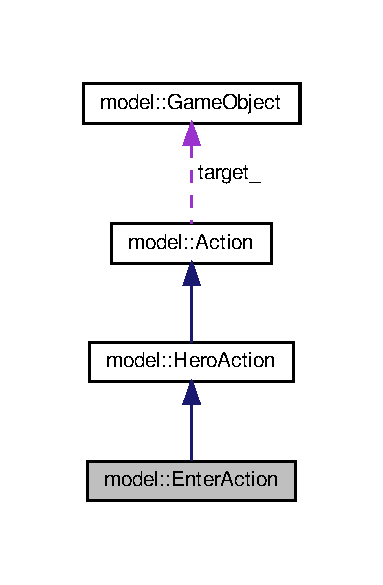
\includegraphics[width=184pt]{classmodel_1_1EnterAction__coll__graph}
\end{center}
\end{figure}
\subsection*{Metody publiczne}
\begin{DoxyCompactItemize}
\item 
\hyperlink{classmodel_1_1EnterAction_ac95609f75be49871c93e2948229f0049}{Enter\+Action} (const \hyperlink{classmodel_1_1GameObject}{Game\+Object} \&target)
\begin{DoxyCompactList}\small\item\em Publiczny konstruktor z parametrem klasy \hyperlink{classmodel_1_1GameObject}{Game\+Object}. \end{DoxyCompactList}\item 
virtual void \hyperlink{classmodel_1_1EnterAction_a0e6f49b42a1c026c421f29193670abeb}{print} ()
\begin{DoxyCompactList}\small\item\em Wirtualna metoda print. \end{DoxyCompactList}\end{DoxyCompactItemize}
\subsection*{Dodatkowe Dziedziczone Składowe}


\subsection{Opis szczegółowy}
Klasa \hyperlink{classmodel_1_1EnterAction}{Enter\+Action}. 

Klasa imitująca klasę akcji wejścia bohatera do danego celu wydanego przez algorytm bota. 

\subsection{Dokumentacja konstruktora i destruktora}
\mbox{\Hypertarget{classmodel_1_1EnterAction_ac95609f75be49871c93e2948229f0049}\label{classmodel_1_1EnterAction_ac95609f75be49871c93e2948229f0049}} 
\index{model\+::\+Enter\+Action@{model\+::\+Enter\+Action}!Enter\+Action@{Enter\+Action}}
\index{Enter\+Action@{Enter\+Action}!model\+::\+Enter\+Action@{model\+::\+Enter\+Action}}
\subsubsection{\texorpdfstring{Enter\+Action()}{EnterAction()}}
{\footnotesize\ttfamily model\+::\+Enter\+Action\+::\+Enter\+Action (\begin{DoxyParamCaption}\item[{const \hyperlink{classmodel_1_1GameObject}{Game\+Object} \&}]{target }\end{DoxyParamCaption})\hspace{0.3cm}{\ttfamily [inline]}}



Publiczny konstruktor z parametrem klasy \hyperlink{classmodel_1_1GameObject}{Game\+Object}. 


\begin{DoxyParams}{Parametry}
{\em target} & stała referencja na obiekt klasy \hyperlink{classmodel_1_1GameObject}{Game\+Object}. \\
\hline
\end{DoxyParams}


\subsection{Dokumentacja funkcji składowych}
\mbox{\Hypertarget{classmodel_1_1EnterAction_a0e6f49b42a1c026c421f29193670abeb}\label{classmodel_1_1EnterAction_a0e6f49b42a1c026c421f29193670abeb}} 
\index{model\+::\+Enter\+Action@{model\+::\+Enter\+Action}!print@{print}}
\index{print@{print}!model\+::\+Enter\+Action@{model\+::\+Enter\+Action}}
\subsubsection{\texorpdfstring{print()}{print()}}
{\footnotesize\ttfamily virtual void model\+::\+Enter\+Action\+::print (\begin{DoxyParamCaption}{ }\end{DoxyParamCaption})\hspace{0.3cm}{\ttfamily [inline]}, {\ttfamily [virtual]}}



Wirtualna metoda print. 

Stosowana jedynie do informacji o zawartości kontenera decyzji 

Reimplementowana z \hyperlink{classmodel_1_1Action_a2955dbb4a69e38a48aa07d730fe2d77c}{model\+::\+Action}.



Dokumentacja dla tej klasy została wygenerowana z pliku\+:\begin{DoxyCompactItemize}
\item 
/home/bartlomiej/eclipse-\/workspace/lab\+\_\+3/src/bot/model/\hyperlink{enter__action_8hpp}{enter\+\_\+action.\+hpp}\end{DoxyCompactItemize}

\hypertarget{classmodel_1_1FightAction}{}\section{Dokumentacja klasy model\+:\+:Fight\+Action}
\label{classmodel_1_1FightAction}\index{model\+::\+Fight\+Action@{model\+::\+Fight\+Action}}


Klasa \hyperlink{classmodel_1_1FightAction}{Fight\+Action}.  




{\ttfamily \#include $<$fight\+\_\+action.\+hpp$>$}



Diagram dziedziczenia dla model\+:\+:Fight\+Action\nopagebreak
\begin{figure}[H]
\begin{center}
\leavevmode
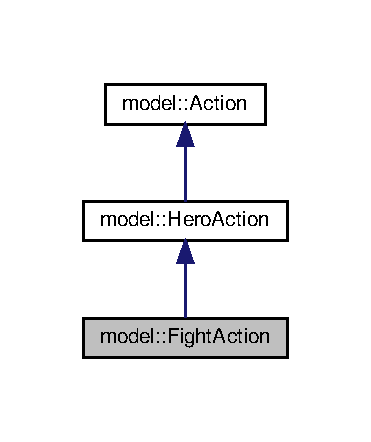
\includegraphics[width=178pt]{classmodel_1_1FightAction__inherit__graph}
\end{center}
\end{figure}


Diagram współpracy dla model\+:\+:Fight\+Action\+:\nopagebreak
\begin{figure}[H]
\begin{center}
\leavevmode
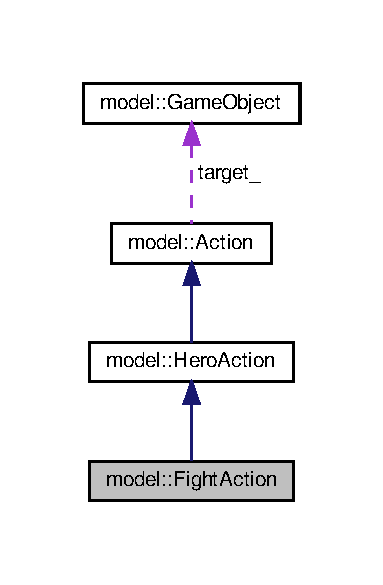
\includegraphics[width=184pt]{classmodel_1_1FightAction__coll__graph}
\end{center}
\end{figure}
\subsection*{Metody publiczne}
\begin{DoxyCompactItemize}
\item 
\hyperlink{classmodel_1_1FightAction_ada818e85e1cc27631dbabe10402b210f}{Fight\+Action} (const \hyperlink{classmodel_1_1GameObject}{Game\+Object} \&target)
\begin{DoxyCompactList}\small\item\em Publiczny konstruktor z parametrem klasy \hyperlink{classmodel_1_1GameObject}{Game\+Object}. \end{DoxyCompactList}\item 
virtual void \hyperlink{classmodel_1_1FightAction_a416846e68a9aa998412da4d439dbc6cc}{print} ()
\begin{DoxyCompactList}\small\item\em Wirtualna metoda print. \end{DoxyCompactList}\end{DoxyCompactItemize}
\subsection*{Dodatkowe Dziedziczone Składowe}


\subsection{Opis szczegółowy}
Klasa \hyperlink{classmodel_1_1FightAction}{Fight\+Action}. 

Klasa imitująca klasę akcji walki z danym celem wydaną przez algorytm bota. 

\subsection{Dokumentacja konstruktora i destruktora}
\mbox{\Hypertarget{classmodel_1_1FightAction_ada818e85e1cc27631dbabe10402b210f}\label{classmodel_1_1FightAction_ada818e85e1cc27631dbabe10402b210f}} 
\index{model\+::\+Fight\+Action@{model\+::\+Fight\+Action}!Fight\+Action@{Fight\+Action}}
\index{Fight\+Action@{Fight\+Action}!model\+::\+Fight\+Action@{model\+::\+Fight\+Action}}
\subsubsection{\texorpdfstring{Fight\+Action()}{FightAction()}}
{\footnotesize\ttfamily model\+::\+Fight\+Action\+::\+Fight\+Action (\begin{DoxyParamCaption}\item[{const \hyperlink{classmodel_1_1GameObject}{Game\+Object} \&}]{target }\end{DoxyParamCaption})\hspace{0.3cm}{\ttfamily [inline]}}



Publiczny konstruktor z parametrem klasy \hyperlink{classmodel_1_1GameObject}{Game\+Object}. 


\begin{DoxyParams}{Parametry}
{\em target} & stała referencja na obiekt klasy \hyperlink{classmodel_1_1GameObject}{Game\+Object}. \\
\hline
\end{DoxyParams}


\subsection{Dokumentacja funkcji składowych}
\mbox{\Hypertarget{classmodel_1_1FightAction_a416846e68a9aa998412da4d439dbc6cc}\label{classmodel_1_1FightAction_a416846e68a9aa998412da4d439dbc6cc}} 
\index{model\+::\+Fight\+Action@{model\+::\+Fight\+Action}!print@{print}}
\index{print@{print}!model\+::\+Fight\+Action@{model\+::\+Fight\+Action}}
\subsubsection{\texorpdfstring{print()}{print()}}
{\footnotesize\ttfamily virtual void model\+::\+Fight\+Action\+::print (\begin{DoxyParamCaption}{ }\end{DoxyParamCaption})\hspace{0.3cm}{\ttfamily [inline]}, {\ttfamily [virtual]}}



Wirtualna metoda print. 

Stosowana jedynie do informacji o zawartości kontenera decyzji 

Reimplementowana z \hyperlink{classmodel_1_1Action_a2955dbb4a69e38a48aa07d730fe2d77c}{model\+::\+Action}.



Dokumentacja dla tej klasy została wygenerowana z pliku\+:\begin{DoxyCompactItemize}
\item 
/home/bartlomiej/eclipse-\/workspace/lab\+\_\+3/src/bot/model/\hyperlink{fight__action_8hpp}{fight\+\_\+action.\+hpp}\end{DoxyCompactItemize}

\hypertarget{classmodel_1_1GameObject}{}\section{Dokumentacja klasy model\+:\+:Game\+Object}
\label{classmodel_1_1GameObject}\index{model\+::\+Game\+Object@{model\+::\+Game\+Object}}


Klasa \hyperlink{classmodel_1_1GameObject}{Game\+Object}.  




{\ttfamily \#include $<$game\+\_\+object.\+hpp$>$}



Diagram dziedziczenia dla model\+:\+:Game\+Object\nopagebreak
\begin{figure}[H]
\begin{center}
\leavevmode
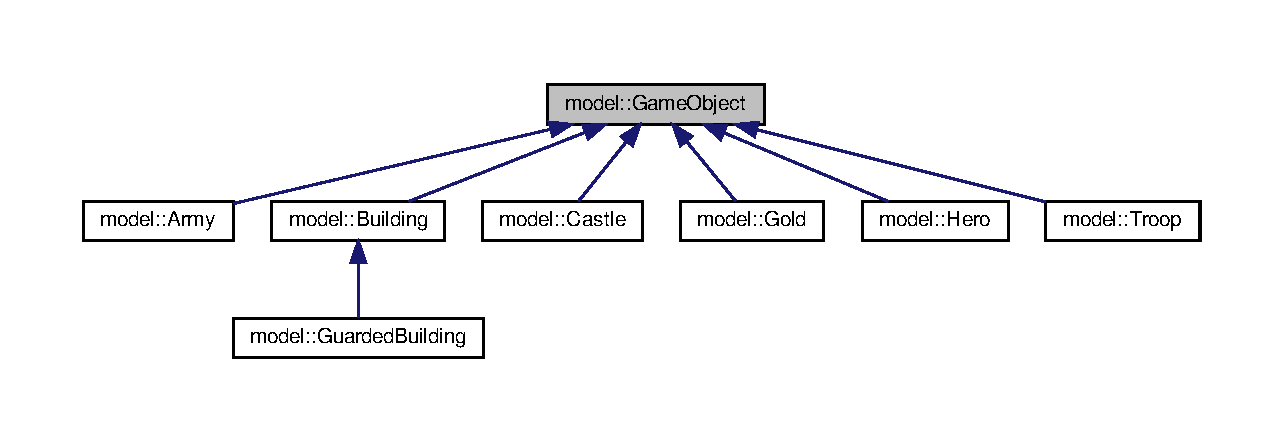
\includegraphics[width=350pt]{classmodel_1_1GameObject__inherit__graph}
\end{center}
\end{figure}
\subsection*{Metody publiczne}
\begin{DoxyCompactItemize}
\item 
\hyperlink{classmodel_1_1GameObject_aec3d26647ae22d325282e07b4391de0a}{Game\+Object} (int x=0, int y=0)
\begin{DoxyCompactList}\small\item\em Publiczny konstruktor domyślny. \end{DoxyCompactList}\item 
\hyperlink{classmodel_1_1GameObject_add23441faffd638c0cba4950b8555364}{Game\+Object} (const \hyperlink{classmodel_1_1GameObject}{Game\+Object} \&object)
\begin{DoxyCompactList}\small\item\em Publiczny konstruktor kopiujący. \end{DoxyCompactList}\item 
\mbox{\Hypertarget{classmodel_1_1GameObject_a3ed9274eb807ef622cf50ebe6126f297}\label{classmodel_1_1GameObject_a3ed9274eb807ef622cf50ebe6126f297}} 
void \hyperlink{classmodel_1_1GameObject_a3ed9274eb807ef622cf50ebe6126f297}{set\+\_\+coordinates} (int x, int y)
\begin{DoxyCompactList}\small\item\em Setter ustawia współrzędne obiektu gry. \end{DoxyCompactList}\item 
\mbox{\Hypertarget{classmodel_1_1GameObject_a7dd3d6798cbc6182908c8181114c8383}\label{classmodel_1_1GameObject_a7dd3d6798cbc6182908c8181114c8383}} 
int \hyperlink{classmodel_1_1GameObject_a7dd3d6798cbc6182908c8181114c8383}{get\+\_\+x} () const
\begin{DoxyCompactList}\small\item\em Getter zwraca współrzędną x. \end{DoxyCompactList}\item 
\mbox{\Hypertarget{classmodel_1_1GameObject_ac883bfccb78ec3e689d1672755bf44f8}\label{classmodel_1_1GameObject_ac883bfccb78ec3e689d1672755bf44f8}} 
int \hyperlink{classmodel_1_1GameObject_ac883bfccb78ec3e689d1672755bf44f8}{get\+\_\+y} () const
\begin{DoxyCompactList}\small\item\em Getter zwraca współrzędną y. \end{DoxyCompactList}\item 
\mbox{\Hypertarget{classmodel_1_1GameObject_a294f5a3a05529858758edba9f9f02ee3}\label{classmodel_1_1GameObject_a294f5a3a05529858758edba9f9f02ee3}} 
int \hyperlink{classmodel_1_1GameObject_a294f5a3a05529858758edba9f9f02ee3}{get\+\_\+distance} (const \hyperlink{classmodel_1_1GameObject}{Game\+Object} \&destination) const
\begin{DoxyCompactList}\small\item\em Funkcja obliczająca odległość pomiędzy obiektami; pierwiastek z sumy kwadratów. \end{DoxyCompactList}\item 
\mbox{\Hypertarget{classmodel_1_1GameObject_acfd1cc777708e9db44f59716db36c486}\label{classmodel_1_1GameObject_acfd1cc777708e9db44f59716db36c486}} 
virtual \hyperlink{classmodel_1_1GameObject_acfd1cc777708e9db44f59716db36c486}{$\sim$\+Game\+Object} ()
\begin{DoxyCompactList}\small\item\em Wirtualny destruktor. \end{DoxyCompactList}\end{DoxyCompactItemize}


\subsection{Opis szczegółowy}
Klasa \hyperlink{classmodel_1_1GameObject}{Game\+Object}. 

Klasa obiektu gry w rozumieniu bota; po niej dziedziczą wszystkie obiekty stanu gry. 

\subsection{Dokumentacja konstruktora i destruktora}
\mbox{\Hypertarget{classmodel_1_1GameObject_aec3d26647ae22d325282e07b4391de0a}\label{classmodel_1_1GameObject_aec3d26647ae22d325282e07b4391de0a}} 
\index{model\+::\+Game\+Object@{model\+::\+Game\+Object}!Game\+Object@{Game\+Object}}
\index{Game\+Object@{Game\+Object}!model\+::\+Game\+Object@{model\+::\+Game\+Object}}
\subsubsection{\texorpdfstring{Game\+Object()}{GameObject()}\hspace{0.1cm}{\footnotesize\ttfamily [1/2]}}
{\footnotesize\ttfamily model\+::\+Game\+Object\+::\+Game\+Object (\begin{DoxyParamCaption}\item[{int}]{x = {\ttfamily 0},  }\item[{int}]{y = {\ttfamily 0} }\end{DoxyParamCaption})\hspace{0.3cm}{\ttfamily [inline]}}



Publiczny konstruktor domyślny. 


\begin{DoxyParams}{Parametry}
{\em x} & współrzędna x. \\
\hline
{\em y} & współrzędna y. \\
\hline
\end{DoxyParams}
\mbox{\Hypertarget{classmodel_1_1GameObject_add23441faffd638c0cba4950b8555364}\label{classmodel_1_1GameObject_add23441faffd638c0cba4950b8555364}} 
\index{model\+::\+Game\+Object@{model\+::\+Game\+Object}!Game\+Object@{Game\+Object}}
\index{Game\+Object@{Game\+Object}!model\+::\+Game\+Object@{model\+::\+Game\+Object}}
\subsubsection{\texorpdfstring{Game\+Object()}{GameObject()}\hspace{0.1cm}{\footnotesize\ttfamily [2/2]}}
{\footnotesize\ttfamily model\+::\+Game\+Object\+::\+Game\+Object (\begin{DoxyParamCaption}\item[{const \hyperlink{classmodel_1_1GameObject}{Game\+Object} \&}]{object }\end{DoxyParamCaption})\hspace{0.3cm}{\ttfamily [inline]}}



Publiczny konstruktor kopiujący. 


\begin{DoxyParams}{Parametry}
{\em object} & stała referencja na obiekt klasy \hyperlink{classmodel_1_1GameObject}{Game\+Object} \\
\hline
\end{DoxyParams}


Dokumentacja dla tej klasy została wygenerowana z pliku\+:\begin{DoxyCompactItemize}
\item 
/home/bartlomiej/eclipse-\/workspace/lab\+\_\+3/src/bot/model/\hyperlink{game__object_8hpp}{game\+\_\+object.\+hpp}\end{DoxyCompactItemize}

\hypertarget{structmodel_1_1GameState}{}\section{Dokumentacja struktury model\+:\+:Game\+State}
\label{structmodel_1_1GameState}\index{model\+::\+Game\+State@{model\+::\+Game\+State}}


Struktura \hyperlink{structmodel_1_1GameState}{Game\+State}.  




{\ttfamily \#include $<$game\+\_\+state.\+hpp$>$}



Diagram współpracy dla model\+:\+:Game\+State\+:\nopagebreak
\begin{figure}[H]
\begin{center}
\leavevmode
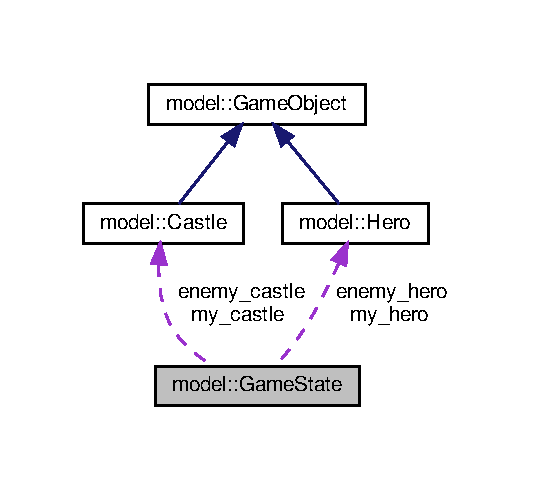
\includegraphics[width=256pt]{structmodel_1_1GameState__coll__graph}
\end{center}
\end{figure}
\subsection*{Atrybuty publiczne}
\begin{DoxyCompactItemize}
\item 
\mbox{\Hypertarget{structmodel_1_1GameState_a4117472d16817fad15015f2fdd29f792}\label{structmodel_1_1GameState_a4117472d16817fad15015f2fdd29f792}} 
\hyperlink{classmodel_1_1Hero}{Hero} \hyperlink{structmodel_1_1GameState_a4117472d16817fad15015f2fdd29f792}{my\+\_\+hero}
\begin{DoxyCompactList}\small\item\em Składowa struktury; bohater bota klasy \hyperlink{classmodel_1_1Hero}{Hero}. \end{DoxyCompactList}\item 
\mbox{\Hypertarget{structmodel_1_1GameState_a460be6a1f98dcfad818686f241c35ad6}\label{structmodel_1_1GameState_a460be6a1f98dcfad818686f241c35ad6}} 
\hyperlink{classmodel_1_1Hero}{Hero} \hyperlink{structmodel_1_1GameState_a460be6a1f98dcfad818686f241c35ad6}{enemy\+\_\+hero}
\begin{DoxyCompactList}\small\item\em Składowa struktury; bohater przeciwnika klasy \hyperlink{classmodel_1_1Hero}{Hero}. \end{DoxyCompactList}\item 
\mbox{\Hypertarget{structmodel_1_1GameState_a877bf51dc420a95db8bfd8ecc2d02131}\label{structmodel_1_1GameState_a877bf51dc420a95db8bfd8ecc2d02131}} 
\hyperlink{classmodel_1_1Castle}{Castle} \hyperlink{structmodel_1_1GameState_a877bf51dc420a95db8bfd8ecc2d02131}{my\+\_\+castle}
\begin{DoxyCompactList}\small\item\em Składowa struktury; zamek bota klasy \hyperlink{classmodel_1_1Castle}{Castle}. \end{DoxyCompactList}\item 
\mbox{\Hypertarget{structmodel_1_1GameState_a32af616a72b81ca3dfff1afa5e7ecd39}\label{structmodel_1_1GameState_a32af616a72b81ca3dfff1afa5e7ecd39}} 
\hyperlink{classmodel_1_1Castle}{Castle} \hyperlink{structmodel_1_1GameState_a32af616a72b81ca3dfff1afa5e7ecd39}{enemy\+\_\+castle}
\begin{DoxyCompactList}\small\item\em Składowa struktury; zamek przeciwnika klasy \hyperlink{classmodel_1_1Castle}{Castle}. \end{DoxyCompactList}\item 
\mbox{\Hypertarget{structmodel_1_1GameState_abf5bb9d70022de2c70b5e575964d516d}\label{structmodel_1_1GameState_abf5bb9d70022de2c70b5e575964d516d}} 
\hyperlink{building_8hpp_a73ce6a7004694882057ce332b6741811}{Building\+Container} \hyperlink{structmodel_1_1GameState_abf5bb9d70022de2c70b5e575964d516d}{buildings}
\begin{DoxyCompactList}\small\item\em Składowa struktury; budynki na mapie jako wektor klasy \hyperlink{classmodel_1_1Building}{Building}. \end{DoxyCompactList}\item 
\mbox{\Hypertarget{structmodel_1_1GameState_a065ec91ab324eaf7e3a1bca69bb9fe68}\label{structmodel_1_1GameState_a065ec91ab324eaf7e3a1bca69bb9fe68}} 
\hyperlink{guarded__building_8hpp_a4c05c1c79b1b5f3bbb54b04c990d53ce}{Guarded\+Building\+Container} \hyperlink{structmodel_1_1GameState_a065ec91ab324eaf7e3a1bca69bb9fe68}{guarded\+\_\+buildings}
\begin{DoxyCompactList}\small\item\em Składowa struktury; strzeżone budynki na mapie jako wektor klasy \hyperlink{classmodel_1_1GuardedBuilding}{Guarded\+Building}. \end{DoxyCompactList}\item 
\mbox{\Hypertarget{structmodel_1_1GameState_a88fdf34d6fbb8cdc7bbbacd5a2732ce6}\label{structmodel_1_1GameState_a88fdf34d6fbb8cdc7bbbacd5a2732ce6}} 
\hyperlink{gold_8hpp_acc4c719f33d9505529826f5d8fe38836}{Gold\+Container} \hyperlink{structmodel_1_1GameState_a88fdf34d6fbb8cdc7bbbacd5a2732ce6}{map\+\_\+gold}
\begin{DoxyCompactList}\small\item\em Składowa struktury; złoto na mapie jako wektor klasy \hyperlink{classmodel_1_1Gold}{Gold}. \end{DoxyCompactList}\item 
\mbox{\Hypertarget{structmodel_1_1GameState_aec56cde504fbd48e60a504d6441d1dae}\label{structmodel_1_1GameState_aec56cde504fbd48e60a504d6441d1dae}} 
\hyperlink{troop_8hpp_a98a8449fdd332f3100611e4f42735f26}{Troop\+Container} \hyperlink{structmodel_1_1GameState_aec56cde504fbd48e60a504d6441d1dae}{map\+\_\+troops}
\begin{DoxyCompactList}\small\item\em Składowa struktury; oddziały na mapie jako wektor klasy \hyperlink{classmodel_1_1Troop}{Troop}. \end{DoxyCompactList}\end{DoxyCompactItemize}


\subsection{Opis szczegółowy}
Struktura \hyperlink{structmodel_1_1GameState}{Game\+State}. 

Struktura stanu gry w rozumieniu bota; zawiera wszystkie obiekty będące w rozgrywce. 

Dokumentacja dla tej struktury została wygenerowana z pliku\+:\begin{DoxyCompactItemize}
\item 
/home/bartlomiej/eclipse-\/workspace/lab\+\_\+3/src/bot/model/\hyperlink{game__state_8hpp}{game\+\_\+state.\+hpp}\end{DoxyCompactItemize}

\hypertarget{classmodel_1_1Gold}{}\section{Dokumentacja klasy model\+:\+:Gold}
\label{classmodel_1_1Gold}\index{model\+::\+Gold@{model\+::\+Gold}}


Klasa \hyperlink{classmodel_1_1Gold}{Gold}.  




{\ttfamily \#include $<$gold.\+hpp$>$}



Diagram dziedziczenia dla model\+:\+:Gold\nopagebreak
\begin{figure}[H]
\begin{center}
\leavevmode
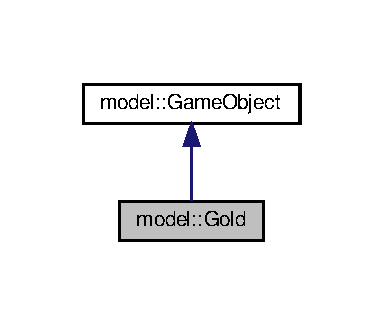
\includegraphics[width=184pt]{classmodel_1_1Gold__inherit__graph}
\end{center}
\end{figure}


Diagram współpracy dla model\+:\+:Gold\+:\nopagebreak
\begin{figure}[H]
\begin{center}
\leavevmode
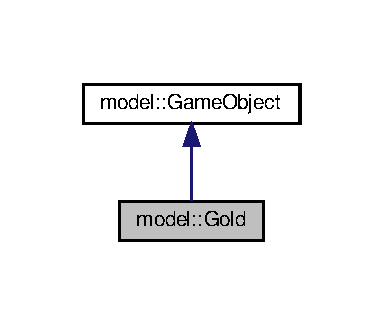
\includegraphics[width=184pt]{classmodel_1_1Gold__coll__graph}
\end{center}
\end{figure}
\subsection*{Metody publiczne}
\begin{DoxyCompactItemize}
\item 
\hyperlink{classmodel_1_1Gold_af03300ab94b3c7ac512d01bc077e3b8c}{Gold} (int quantity=0, int x=0, int y=0)
\begin{DoxyCompactList}\small\item\em Publiczny konstruktor domyślny. \end{DoxyCompactList}\item 
\mbox{\Hypertarget{classmodel_1_1Gold_a12dc623fc71413530868aff26f81981d}\label{classmodel_1_1Gold_a12dc623fc71413530868aff26f81981d}} 
int \hyperlink{classmodel_1_1Gold_a12dc623fc71413530868aff26f81981d}{get\+\_\+quantity} ()
\begin{DoxyCompactList}\small\item\em Getter zwraca ilość złota. \end{DoxyCompactList}\end{DoxyCompactItemize}


\subsection{Opis szczegółowy}
Klasa \hyperlink{classmodel_1_1Gold}{Gold}. 

Klasa złota w rozumieniu bota, będąca obiektem gry, więc publicznie dziedzicząca po klasie \hyperlink{classmodel_1_1GameObject}{Game\+Object}. 

\subsection{Dokumentacja konstruktora i destruktora}
\mbox{\Hypertarget{classmodel_1_1Gold_af03300ab94b3c7ac512d01bc077e3b8c}\label{classmodel_1_1Gold_af03300ab94b3c7ac512d01bc077e3b8c}} 
\index{model\+::\+Gold@{model\+::\+Gold}!Gold@{Gold}}
\index{Gold@{Gold}!model\+::\+Gold@{model\+::\+Gold}}
\subsubsection{\texorpdfstring{Gold()}{Gold()}}
{\footnotesize\ttfamily model\+::\+Gold\+::\+Gold (\begin{DoxyParamCaption}\item[{int}]{quantity = {\ttfamily 0},  }\item[{int}]{x = {\ttfamily 0},  }\item[{int}]{y = {\ttfamily 0} }\end{DoxyParamCaption})\hspace{0.3cm}{\ttfamily [inline]}}



Publiczny konstruktor domyślny. 


\begin{DoxyParams}{Parametry}
{\em quantity} & ilość złota. \\
\hline
{\em x} & współrzędna x. \\
\hline
{\em y} & współrzędna y. \\
\hline
\end{DoxyParams}


Dokumentacja dla tej klasy została wygenerowana z pliku\+:\begin{DoxyCompactItemize}
\item 
/home/bartlomiej/eclipse-\/workspace/lab\+\_\+3/src/bot/model/\hyperlink{gold_8hpp}{gold.\+hpp}\end{DoxyCompactItemize}

\hypertarget{classmodel_1_1GuardedBuilding}{}\section{Dokumentacja klasy model\+:\+:Guarded\+Building}
\label{classmodel_1_1GuardedBuilding}\index{model\+::\+Guarded\+Building@{model\+::\+Guarded\+Building}}


Klasa \hyperlink{classmodel_1_1GuardedBuilding}{Guarded\+Building}.  




{\ttfamily \#include $<$guarded\+\_\+building.\+hpp$>$}



Diagram dziedziczenia dla model\+:\+:Guarded\+Building\nopagebreak
\begin{figure}[H]
\begin{center}
\leavevmode
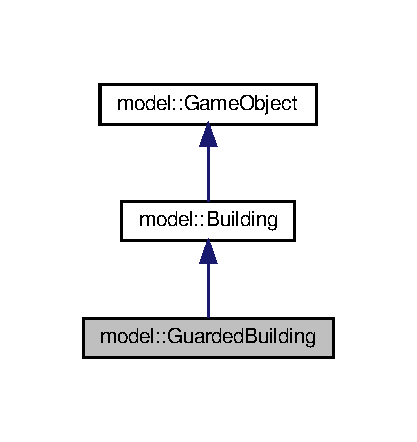
\includegraphics[width=200pt]{classmodel_1_1GuardedBuilding__inherit__graph}
\end{center}
\end{figure}


Diagram współpracy dla model\+:\+:Guarded\+Building\+:\nopagebreak
\begin{figure}[H]
\begin{center}
\leavevmode
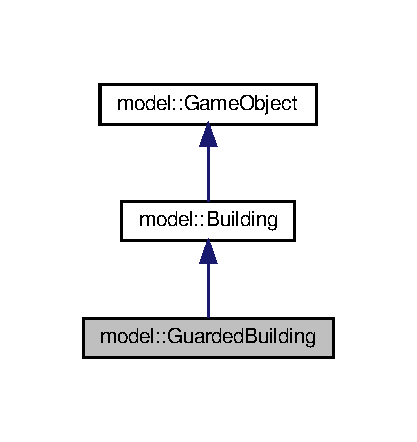
\includegraphics[width=200pt]{classmodel_1_1GuardedBuilding__coll__graph}
\end{center}
\end{figure}
\subsection*{Metody publiczne}
\begin{DoxyCompactItemize}
\item 
\hyperlink{classmodel_1_1GuardedBuilding_acd7faa9dc9d87371b33030b6f0223339}{Guarded\+Building} (\hyperlink{tier_8hpp_a50a003ab1ea342f138c038fabfd1ee55}{Tier} building\+\_\+tier, \hyperlink{status_8hpp_a822822ece62ee330ee656034849df887}{Status} status, int guards\+\_\+num, \hyperlink{tier_8hpp_a50a003ab1ea342f138c038fabfd1ee55}{Tier} guards\+\_\+tier, int x, int y)
\begin{DoxyCompactList}\small\item\em Publiczny konstruktor. \end{DoxyCompactList}\item 
\hyperlink{classmodel_1_1GuardedBuilding_aaf02e02d038198a6cb406505a07ff122}{Guarded\+Building} (int building\+\_\+tier=0, int status=0, int guards\+\_\+num=0, int guards\+\_\+tier=0, int x=0, int y=0)
\begin{DoxyCompactList}\small\item\em Publiczny konstruktor domyślny. \end{DoxyCompactList}\item 
\mbox{\Hypertarget{classmodel_1_1GuardedBuilding_aa8c31f9ba289c4a2d5a69faf29ec6420}\label{classmodel_1_1GuardedBuilding_aa8c31f9ba289c4a2d5a69faf29ec6420}} 
void \hyperlink{classmodel_1_1GuardedBuilding_aa8c31f9ba289c4a2d5a69faf29ec6420}{conquer} ()
\begin{DoxyCompactList}\small\item\em Funkcja zdobycia budynku; ustawia status na przyjazny i liczbę strzegących na 0. \end{DoxyCompactList}\item 
\mbox{\Hypertarget{classmodel_1_1GuardedBuilding_a7c2e4457eb1d29dd7b05268c1c5796e6}\label{classmodel_1_1GuardedBuilding_a7c2e4457eb1d29dd7b05268c1c5796e6}} 
\hyperlink{tier_8hpp_a50a003ab1ea342f138c038fabfd1ee55}{Tier} \hyperlink{classmodel_1_1GuardedBuilding_a7c2e4457eb1d29dd7b05268c1c5796e6}{get\+\_\+guards\+\_\+tier} () const
\begin{DoxyCompactList}\small\item\em Getter zwraca poziom oddziału. \end{DoxyCompactList}\item 
\mbox{\Hypertarget{classmodel_1_1GuardedBuilding_aa06bc4f6b2ab78d37556a1395e6278dc}\label{classmodel_1_1GuardedBuilding_aa06bc4f6b2ab78d37556a1395e6278dc}} 
int \hyperlink{classmodel_1_1GuardedBuilding_aa06bc4f6b2ab78d37556a1395e6278dc}{get\+\_\+guards\+\_\+quantity} () const
\begin{DoxyCompactList}\small\item\em Getter zwraca liczebnośc oddziału. \end{DoxyCompactList}\item 
\mbox{\Hypertarget{classmodel_1_1GuardedBuilding_a0bd614b0fa5b050c6226bc1f986b526f}\label{classmodel_1_1GuardedBuilding_a0bd614b0fa5b050c6226bc1f986b526f}} 
int \hyperlink{classmodel_1_1GuardedBuilding_a0bd614b0fa5b050c6226bc1f986b526f}{count\+\_\+guards\+\_\+force} () const
\begin{DoxyCompactList}\small\item\em Funkcja obliczająca siłę oddziału strzegącego budynek. \end{DoxyCompactList}\end{DoxyCompactItemize}


\subsection{Opis szczegółowy}
Klasa \hyperlink{classmodel_1_1GuardedBuilding}{Guarded\+Building}. 

Klasa strzeżonego budynku w rozumieniu bota, będąca budynkiem, więc publicznie dziedzicząca po klasie \hyperlink{classmodel_1_1Building}{Building}. 

\subsection{Dokumentacja konstruktora i destruktora}
\mbox{\Hypertarget{classmodel_1_1GuardedBuilding_acd7faa9dc9d87371b33030b6f0223339}\label{classmodel_1_1GuardedBuilding_acd7faa9dc9d87371b33030b6f0223339}} 
\index{model\+::\+Guarded\+Building@{model\+::\+Guarded\+Building}!Guarded\+Building@{Guarded\+Building}}
\index{Guarded\+Building@{Guarded\+Building}!model\+::\+Guarded\+Building@{model\+::\+Guarded\+Building}}
\subsubsection{\texorpdfstring{Guarded\+Building()}{GuardedBuilding()}\hspace{0.1cm}{\footnotesize\ttfamily [1/2]}}
{\footnotesize\ttfamily model\+::\+Guarded\+Building\+::\+Guarded\+Building (\begin{DoxyParamCaption}\item[{\hyperlink{tier_8hpp_a50a003ab1ea342f138c038fabfd1ee55}{Tier}}]{building\+\_\+tier,  }\item[{\hyperlink{status_8hpp_a822822ece62ee330ee656034849df887}{Status}}]{status,  }\item[{int}]{guards\+\_\+num,  }\item[{\hyperlink{tier_8hpp_a50a003ab1ea342f138c038fabfd1ee55}{Tier}}]{guards\+\_\+tier,  }\item[{int}]{x,  }\item[{int}]{y }\end{DoxyParamCaption})\hspace{0.3cm}{\ttfamily [inline]}}



Publiczny konstruktor. 


\begin{DoxyParams}{Parametry}
{\em building\+\_\+tier} & poziom budynku klasy enumeracyjnej Tier. \\
\hline
{\em status} & status budynku klasy enumeracyjnej Status. \\
\hline
{\em guards\+\_\+num} & liczebność oddziału. \\
\hline
{\em guards\+\_\+tier} & poziom oddziału strzegącego klasy enumeracyjnej Tier. \\
\hline
{\em x} & współrzędna x. \\
\hline
{\em y} & współrzędna y. \\
\hline
\end{DoxyParams}
\mbox{\Hypertarget{classmodel_1_1GuardedBuilding_aaf02e02d038198a6cb406505a07ff122}\label{classmodel_1_1GuardedBuilding_aaf02e02d038198a6cb406505a07ff122}} 
\index{model\+::\+Guarded\+Building@{model\+::\+Guarded\+Building}!Guarded\+Building@{Guarded\+Building}}
\index{Guarded\+Building@{Guarded\+Building}!model\+::\+Guarded\+Building@{model\+::\+Guarded\+Building}}
\subsubsection{\texorpdfstring{Guarded\+Building()}{GuardedBuilding()}\hspace{0.1cm}{\footnotesize\ttfamily [2/2]}}
{\footnotesize\ttfamily model\+::\+Guarded\+Building\+::\+Guarded\+Building (\begin{DoxyParamCaption}\item[{int}]{building\+\_\+tier = {\ttfamily 0},  }\item[{int}]{status = {\ttfamily 0},  }\item[{int}]{guards\+\_\+num = {\ttfamily 0},  }\item[{int}]{guards\+\_\+tier = {\ttfamily 0},  }\item[{int}]{x = {\ttfamily 0},  }\item[{int}]{y = {\ttfamily 0} }\end{DoxyParamCaption})\hspace{0.3cm}{\ttfamily [inline]}}



Publiczny konstruktor domyślny. 


\begin{DoxyParams}{Parametry}
{\em building\+\_\+tier} & poziom budynku konwertowany do klasy enumeracyjnej Tier. \\
\hline
{\em status} & status budynku konwertowany do klasy enumeracyjnej Status. \\
\hline
{\em guards\+\_\+num} & liczebność oddziału. \\
\hline
{\em guards\+\_\+tier} & poziom oddziału strzegącego konwertowany do klasy enumeracyjnej Tier. \\
\hline
{\em x} & współrzędna x. \\
\hline
{\em y} & współrzędna y. \\
\hline
\end{DoxyParams}


Dokumentacja dla tej klasy została wygenerowana z pliku\+:\begin{DoxyCompactItemize}
\item 
/home/bartlomiej/eclipse-\/workspace/lab\+\_\+3/src/bot/model/\hyperlink{guarded__building_8hpp}{guarded\+\_\+building.\+hpp}\end{DoxyCompactItemize}

\hypertarget{classmodel_1_1Hero}{}\section{Dokumentacja klasy model\+:\+:Hero}
\label{classmodel_1_1Hero}\index{model\+::\+Hero@{model\+::\+Hero}}


Klasa \hyperlink{classmodel_1_1Hero}{Hero}.  




{\ttfamily \#include $<$hero.\+hpp$>$}



Diagram dziedziczenia dla model\+:\+:Hero\nopagebreak
\begin{figure}[H]
\begin{center}
\leavevmode
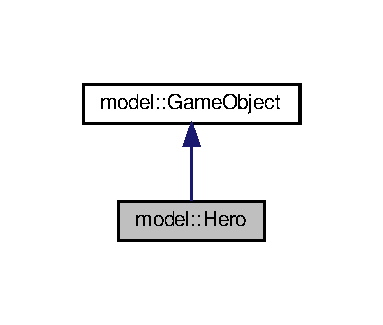
\includegraphics[width=184pt]{classmodel_1_1Hero__inherit__graph}
\end{center}
\end{figure}


Diagram współpracy dla model\+:\+:Hero\+:\nopagebreak
\begin{figure}[H]
\begin{center}
\leavevmode
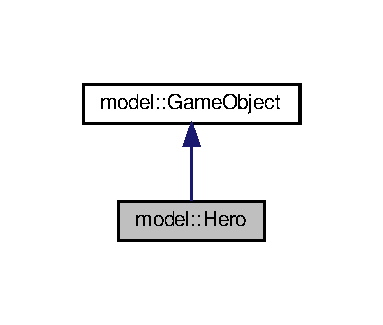
\includegraphics[width=184pt]{classmodel_1_1Hero__coll__graph}
\end{center}
\end{figure}
\subsection*{Metody publiczne}
\begin{DoxyCompactItemize}
\item 
\hyperlink{classmodel_1_1Hero_aeff27a625ef4629d57d2dba7497eb559}{Hero} (int gold=0, int level=0, int high\+\_\+tier\+\_\+army\+\_\+num=0, int mid\+\_\+tier\+\_\+army\+\_\+num=0, int low\+\_\+tier\+\_\+army\+\_\+num=0, int x=0, int y=0, \hyperlink{status_8hpp_a822822ece62ee330ee656034849df887}{Status} status=Status\+::\+N\+E\+U\+T\+R\+AL)
\begin{DoxyCompactList}\small\item\em Publiczny konstruktor domyślny. \end{DoxyCompactList}\item 
\hyperlink{classmodel_1_1Hero_a7c6ec503c2c1409ff11daa69c2d46f9a}{Hero} (const std\+::vector$<$ int $>$ \&params, \hyperlink{status_8hpp_a822822ece62ee330ee656034849df887}{Status} status)
\begin{DoxyCompactList}\small\item\em Publiczny konstruktor. \end{DoxyCompactList}\item 
\mbox{\Hypertarget{classmodel_1_1Hero_abf940dc4b402b8798571272923741f17}\label{classmodel_1_1Hero_abf940dc4b402b8798571272923741f17}} 
void \hyperlink{classmodel_1_1Hero_abf940dc4b402b8798571272923741f17}{travel\+\_\+to} (int x, int y)
\begin{DoxyCompactList}\small\item\em Funkcja podróżuj do; ustawia współrzędne bohatera zgodnie z współrzędnymi celu. \end{DoxyCompactList}\item 
\mbox{\Hypertarget{classmodel_1_1Hero_aa1331373ce8cdc72574cf0c1376cdd7b}\label{classmodel_1_1Hero_aa1331373ce8cdc72574cf0c1376cdd7b}} 
void \hyperlink{classmodel_1_1Hero_aa1331373ce8cdc72574cf0c1376cdd7b}{travel\+\_\+to} (const \hyperlink{classmodel_1_1GameObject}{Game\+Object} \&object)
\begin{DoxyCompactList}\small\item\em Funkcja podróżuj do; ustawia współrzędne bohatera zgodnie z współrzędnymi celu. \end{DoxyCompactList}\item 
\mbox{\Hypertarget{classmodel_1_1Hero_a02d55a332f0355fa1a87c65ea87691ff}\label{classmodel_1_1Hero_a02d55a332f0355fa1a87c65ea87691ff}} 
int \hyperlink{classmodel_1_1Hero_a02d55a332f0355fa1a87c65ea87691ff}{get\+\_\+level} () const
\begin{DoxyCompactList}\small\item\em Getter zwraca poziom bohatera. \end{DoxyCompactList}\item 
\mbox{\Hypertarget{classmodel_1_1Hero_a90e159c929f4c0b5372cdcdc43bda737}\label{classmodel_1_1Hero_a90e159c929f4c0b5372cdcdc43bda737}} 
int \hyperlink{classmodel_1_1Hero_a90e159c929f4c0b5372cdcdc43bda737}{get\+\_\+gold} () const
\begin{DoxyCompactList}\small\item\em Getter zwraca ilość złota bohatera. \end{DoxyCompactList}\item 
\mbox{\Hypertarget{classmodel_1_1Hero_a40675022d006773874a54cc70b0ff84a}\label{classmodel_1_1Hero_a40675022d006773874a54cc70b0ff84a}} 
void \hyperlink{classmodel_1_1Hero_a40675022d006773874a54cc70b0ff84a}{pick\+\_\+up\+\_\+gold} (int quantity)
\begin{DoxyCompactList}\small\item\em Funkcja podnieś złoto; dodaje ilość złota w parametrze do jego własnego złota. \end{DoxyCompactList}\item 
\mbox{\Hypertarget{classmodel_1_1Hero_a1d0c79ec3789a82172a0d2dd1aa0488a}\label{classmodel_1_1Hero_a1d0c79ec3789a82172a0d2dd1aa0488a}} 
int \hyperlink{classmodel_1_1Hero_a1d0c79ec3789a82172a0d2dd1aa0488a}{get\+\_\+high\+\_\+tier\+\_\+army\+\_\+quantity} () const
\begin{DoxyCompactList}\small\item\em Getter zwraca liczbę jednostek wysokiego poziomu w armii bohatera. \end{DoxyCompactList}\item 
\mbox{\Hypertarget{classmodel_1_1Hero_a8828fd7c3ed0b8c1a94ef62022cdce56}\label{classmodel_1_1Hero_a8828fd7c3ed0b8c1a94ef62022cdce56}} 
int \hyperlink{classmodel_1_1Hero_a8828fd7c3ed0b8c1a94ef62022cdce56}{get\+\_\+mid\+\_\+tier\+\_\+army\+\_\+quantity} () const
\begin{DoxyCompactList}\small\item\em Getter zwraca liczbę jednostek średniego poziomu w armii bohatera. \end{DoxyCompactList}\item 
\mbox{\Hypertarget{classmodel_1_1Hero_a39aec53f854130463e7346d29e81f568}\label{classmodel_1_1Hero_a39aec53f854130463e7346d29e81f568}} 
int \hyperlink{classmodel_1_1Hero_a39aec53f854130463e7346d29e81f568}{get\+\_\+low\+\_\+tier\+\_\+army\+\_\+quantity} () const
\begin{DoxyCompactList}\small\item\em Getter zwraca liczbę jednostek niskiego poziomu w armii bohatera. \end{DoxyCompactList}\item 
\mbox{\Hypertarget{classmodel_1_1Hero_a91f42678133f013bf1a4a98f99f850f9}\label{classmodel_1_1Hero_a91f42678133f013bf1a4a98f99f850f9}} 
int \hyperlink{classmodel_1_1Hero_a91f42678133f013bf1a4a98f99f850f9}{get\+\_\+movement\+\_\+points} () const
\begin{DoxyCompactList}\small\item\em Getter zwraca ilość punktów ruchu bohatera. \end{DoxyCompactList}\item 
\mbox{\Hypertarget{classmodel_1_1Hero_a14a9c842962a46c408060370cb8d2617}\label{classmodel_1_1Hero_a14a9c842962a46c408060370cb8d2617}} 
int \hyperlink{classmodel_1_1Hero_a14a9c842962a46c408060370cb8d2617}{count\+\_\+hero\+\_\+force} () const
\begin{DoxyCompactList}\small\item\em Funkcja obliczająca siłę bohatera; mnoży siłę jego armii przez bonus od jego poziomu. \end{DoxyCompactList}\item 
\mbox{\Hypertarget{classmodel_1_1Hero_a833bfd8bbf60219e9576bdb686a43e66}\label{classmodel_1_1Hero_a833bfd8bbf60219e9576bdb686a43e66}} 
void \hyperlink{classmodel_1_1Hero_a833bfd8bbf60219e9576bdb686a43e66}{kill} ()
\begin{DoxyCompactList}\small\item\em Funkcja zabijająca bohatera; ustawia jego status na neutralny. \end{DoxyCompactList}\item 
\mbox{\Hypertarget{classmodel_1_1Hero_a3608f4f287ef07c12125c79cea171002}\label{classmodel_1_1Hero_a3608f4f287ef07c12125c79cea171002}} 
void \hyperlink{classmodel_1_1Hero_a3608f4f287ef07c12125c79cea171002}{kill} (int casualties)
\begin{DoxyCompactList}\small\item\em Funkcja zabijająca część armii bohatera; zabija proporcjonalnie do poziomu oddziałów. \end{DoxyCompactList}\item 
\mbox{\Hypertarget{classmodel_1_1Hero_a65710a95b0aeeb35431e42aad6f5e4df}\label{classmodel_1_1Hero_a65710a95b0aeeb35431e42aad6f5e4df}} 
bool \hyperlink{classmodel_1_1Hero_a65710a95b0aeeb35431e42aad6f5e4df}{is\+\_\+alive} () const
\begin{DoxyCompactList}\small\item\em Funkcja zwraca wartośc logiczą czy bohater żyje czy nie. \end{DoxyCompactList}\end{DoxyCompactItemize}
\subsection*{Statyczne atrybuty publiczne}
\begin{DoxyCompactItemize}
\item 
\mbox{\Hypertarget{classmodel_1_1Hero_ab8a93189dfa42527906e6d66cdfd2eef}\label{classmodel_1_1Hero_ab8a93189dfa42527906e6d66cdfd2eef}} 
static const int \hyperlink{classmodel_1_1Hero_ab8a93189dfa42527906e6d66cdfd2eef}{M\+O\+V\+E\+M\+E\+N\+T\+\_\+\+P\+O\+I\+N\+TS} = 5
\begin{DoxyCompactList}\small\item\em Statyczna stała; punkty ruchu bohatera. \end{DoxyCompactList}\item 
\mbox{\Hypertarget{classmodel_1_1Hero_a24257807504890a7d302f7f2a4c66298}\label{classmodel_1_1Hero_a24257807504890a7d302f7f2a4c66298}} 
static constexpr double \hyperlink{classmodel_1_1Hero_a24257807504890a7d302f7f2a4c66298}{M\+O\+V\+E\+M\+E\+N\+T\+\_\+\+P\+O\+I\+N\+T\+S\+\_\+\+L\+E\+V\+E\+L\+\_\+\+B\+O\+N\+US} = 0.\+4
\begin{DoxyCompactList}\small\item\em Statyczna stała; bonus do punktów ruchu od poziomu bohatera. \end{DoxyCompactList}\item 
\mbox{\Hypertarget{classmodel_1_1Hero_a2d17ca3068a51a516a7b3782da536366}\label{classmodel_1_1Hero_a2d17ca3068a51a516a7b3782da536366}} 
static constexpr double \hyperlink{classmodel_1_1Hero_a2d17ca3068a51a516a7b3782da536366}{A\+R\+M\+Y\+F\+O\+R\+C\+E\+\_\+\+F\+A\+C\+T\+OR} = 0.\+05
\begin{DoxyCompactList}\small\item\em Statyczna stała; wpółczynnik bonusu do siły armii od poziomu bohatera. \end{DoxyCompactList}\item 
\mbox{\Hypertarget{classmodel_1_1Hero_aeb81d3ed857c6f2d0cb3e15ce9931bdd}\label{classmodel_1_1Hero_aeb81d3ed857c6f2d0cb3e15ce9931bdd}} 
static constexpr double \hyperlink{classmodel_1_1Hero_aeb81d3ed857c6f2d0cb3e15ce9931bdd}{C\+A\+S\+U\+A\+L\+T\+I\+E\+S\+\_\+\+F\+A\+C\+T\+OR} = 0.\+33
\begin{DoxyCompactList}\small\item\em Statyczna stała; współczynnik strat w walce oddziałów bohatera. \end{DoxyCompactList}\end{DoxyCompactItemize}


\subsection{Opis szczegółowy}
Klasa \hyperlink{classmodel_1_1Hero}{Hero}. 

Klasa bohatera w rozumieniu bota, będąca obiektem gry, więc publicznie dziedzicząca po klasie \hyperlink{classmodel_1_1GameObject}{Game\+Object}. 

\subsection{Dokumentacja konstruktora i destruktora}
\mbox{\Hypertarget{classmodel_1_1Hero_aeff27a625ef4629d57d2dba7497eb559}\label{classmodel_1_1Hero_aeff27a625ef4629d57d2dba7497eb559}} 
\index{model\+::\+Hero@{model\+::\+Hero}!Hero@{Hero}}
\index{Hero@{Hero}!model\+::\+Hero@{model\+::\+Hero}}
\subsubsection{\texorpdfstring{Hero()}{Hero()}\hspace{0.1cm}{\footnotesize\ttfamily [1/2]}}
{\footnotesize\ttfamily model\+::\+Hero\+::\+Hero (\begin{DoxyParamCaption}\item[{int}]{gold = {\ttfamily 0},  }\item[{int}]{level = {\ttfamily 0},  }\item[{int}]{high\+\_\+tier\+\_\+army\+\_\+num = {\ttfamily 0},  }\item[{int}]{mid\+\_\+tier\+\_\+army\+\_\+num = {\ttfamily 0},  }\item[{int}]{low\+\_\+tier\+\_\+army\+\_\+num = {\ttfamily 0},  }\item[{int}]{x = {\ttfamily 0},  }\item[{int}]{y = {\ttfamily 0},  }\item[{\hyperlink{status_8hpp_a822822ece62ee330ee656034849df887}{Status}}]{status = {\ttfamily Status\+:\+:NEUTRAL} }\end{DoxyParamCaption})\hspace{0.3cm}{\ttfamily [inline]}}



Publiczny konstruktor domyślny. 


\begin{DoxyParams}{Parametry}
{\em gold} & ilość złota bohatera. \\
\hline
{\em level} & numer poziomu boharera. \\
\hline
{\em high\+\_\+tier\+\_\+army\+\_\+num} & liczba jednostek wysokiego poziomu w armii bohatera. \\
\hline
{\em mid\+\_\+tier\+\_\+army\+\_\+num} & liczba jednostek średniego poziomu w armii bohatera. \\
\hline
{\em low\+\_\+tier\+\_\+army\+\_\+num} & liczba jednostek niskiego poziomu w armii bohatera. \\
\hline
{\em status} & status bohatera. \\
\hline
{\em x} & współrzędna x. \\
\hline
{\em y} & współrzędna y. \\
\hline
\end{DoxyParams}
\mbox{\Hypertarget{classmodel_1_1Hero_a7c6ec503c2c1409ff11daa69c2d46f9a}\label{classmodel_1_1Hero_a7c6ec503c2c1409ff11daa69c2d46f9a}} 
\index{model\+::\+Hero@{model\+::\+Hero}!Hero@{Hero}}
\index{Hero@{Hero}!model\+::\+Hero@{model\+::\+Hero}}
\subsubsection{\texorpdfstring{Hero()}{Hero()}\hspace{0.1cm}{\footnotesize\ttfamily [2/2]}}
{\footnotesize\ttfamily model\+::\+Hero\+::\+Hero (\begin{DoxyParamCaption}\item[{const std\+::vector$<$ int $>$ \&}]{params,  }\item[{\hyperlink{status_8hpp_a822822ece62ee330ee656034849df887}{Status}}]{status }\end{DoxyParamCaption})\hspace{0.3cm}{\ttfamily [inline]}}



Publiczny konstruktor. 


\begin{DoxyParams}{Parametry}
{\em params} & wektor parametrów integerowych. \\
\hline
{\em status} & status bohatera. \\
\hline
\end{DoxyParams}


Dokumentacja dla tej klasy została wygenerowana z pliku\+:\begin{DoxyCompactItemize}
\item 
/home/bartlomiej/eclipse-\/workspace/lab\+\_\+3/src/bot/model/\hyperlink{hero_8hpp}{hero.\+hpp}\end{DoxyCompactItemize}

\hypertarget{classmodel_1_1HeroAction}{}\section{Dokumentacja klasy model\+:\+:Hero\+Action}
\label{classmodel_1_1HeroAction}\index{model\+::\+Hero\+Action@{model\+::\+Hero\+Action}}


Klasa \hyperlink{classmodel_1_1HeroAction}{Hero\+Action}.  




{\ttfamily \#include $<$hero\+\_\+action.\+hpp$>$}



Diagram dziedziczenia dla model\+:\+:Hero\+Action\nopagebreak
\begin{figure}[H]
\begin{center}
\leavevmode
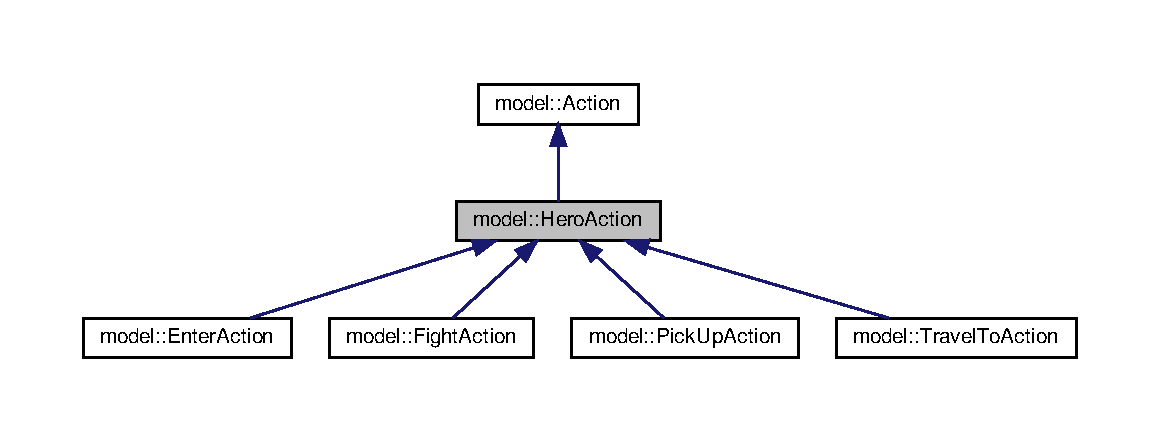
\includegraphics[width=350pt]{classmodel_1_1HeroAction__inherit__graph}
\end{center}
\end{figure}


Diagram współpracy dla model\+:\+:Hero\+Action\+:\nopagebreak
\begin{figure}[H]
\begin{center}
\leavevmode
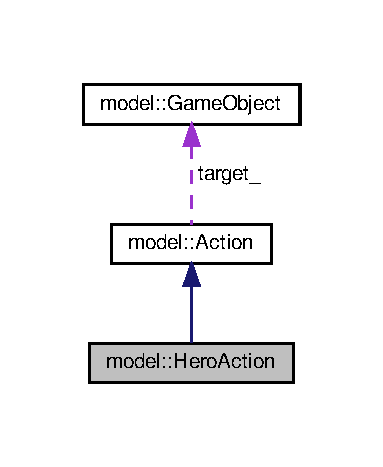
\includegraphics[width=184pt]{classmodel_1_1HeroAction__coll__graph}
\end{center}
\end{figure}
\subsection*{Metody publiczne}
\begin{DoxyCompactItemize}
\item 
\hyperlink{classmodel_1_1HeroAction_a7ec63672d81f1322090b9f7e5a4fb583}{Hero\+Action} (const \hyperlink{classmodel_1_1GameObject}{Game\+Object} \&target)
\begin{DoxyCompactList}\small\item\em Publiczny konstruktor z parametrem klasy \hyperlink{classmodel_1_1GameObject}{Game\+Object}. \end{DoxyCompactList}\item 
\mbox{\Hypertarget{classmodel_1_1HeroAction_acfbfe4eb033779b9ca057cc520896136}\label{classmodel_1_1HeroAction_acfbfe4eb033779b9ca057cc520896136}} 
virtual \hyperlink{classmodel_1_1HeroAction_acfbfe4eb033779b9ca057cc520896136}{$\sim$\+Hero\+Action} ()
\begin{DoxyCompactList}\small\item\em Wirtualny destruktor. \end{DoxyCompactList}\end{DoxyCompactItemize}
\subsection*{Dodatkowe Dziedziczone Składowe}


\subsection{Opis szczegółowy}
Klasa \hyperlink{classmodel_1_1HeroAction}{Hero\+Action}. 

Klasa bazowa dla akcji bohatera wydanych przez algorytm bota. 

\subsection{Dokumentacja konstruktora i destruktora}
\mbox{\Hypertarget{classmodel_1_1HeroAction_a7ec63672d81f1322090b9f7e5a4fb583}\label{classmodel_1_1HeroAction_a7ec63672d81f1322090b9f7e5a4fb583}} 
\index{model\+::\+Hero\+Action@{model\+::\+Hero\+Action}!Hero\+Action@{Hero\+Action}}
\index{Hero\+Action@{Hero\+Action}!model\+::\+Hero\+Action@{model\+::\+Hero\+Action}}
\subsubsection{\texorpdfstring{Hero\+Action()}{HeroAction()}}
{\footnotesize\ttfamily model\+::\+Hero\+Action\+::\+Hero\+Action (\begin{DoxyParamCaption}\item[{const \hyperlink{classmodel_1_1GameObject}{Game\+Object} \&}]{target }\end{DoxyParamCaption})\hspace{0.3cm}{\ttfamily [inline]}, {\ttfamily [explicit]}}



Publiczny konstruktor z parametrem klasy \hyperlink{classmodel_1_1GameObject}{Game\+Object}. 


\begin{DoxyParams}{Parametry}
{\em target} & stała referencja na obiekt klasy \hyperlink{classmodel_1_1GameObject}{Game\+Object}. \\
\hline
\end{DoxyParams}


Dokumentacja dla tej klasy została wygenerowana z pliku\+:\begin{DoxyCompactItemize}
\item 
/home/bartlomiej/eclipse-\/workspace/lab\+\_\+3/src/bot/model/\hyperlink{hero__action_8hpp}{hero\+\_\+action.\+hpp}\end{DoxyCompactItemize}

\hypertarget{classmodel_1_1PickUpAction}{}\section{Dokumentacja klasy model\+:\+:Pick\+Up\+Action}
\label{classmodel_1_1PickUpAction}\index{model\+::\+Pick\+Up\+Action@{model\+::\+Pick\+Up\+Action}}


Klasa \hyperlink{classmodel_1_1PickUpAction}{Pick\+Up\+Action}.  




{\ttfamily \#include $<$pick\+\_\+up\+\_\+action.\+hpp$>$}



Diagram dziedziczenia dla model\+:\+:Pick\+Up\+Action\nopagebreak
\begin{figure}[H]
\begin{center}
\leavevmode
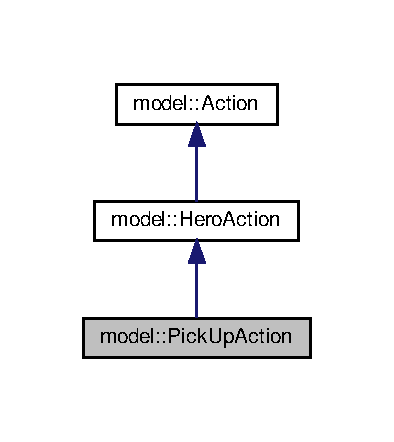
\includegraphics[width=189pt]{classmodel_1_1PickUpAction__inherit__graph}
\end{center}
\end{figure}


Diagram współpracy dla model\+:\+:Pick\+Up\+Action\+:\nopagebreak
\begin{figure}[H]
\begin{center}
\leavevmode
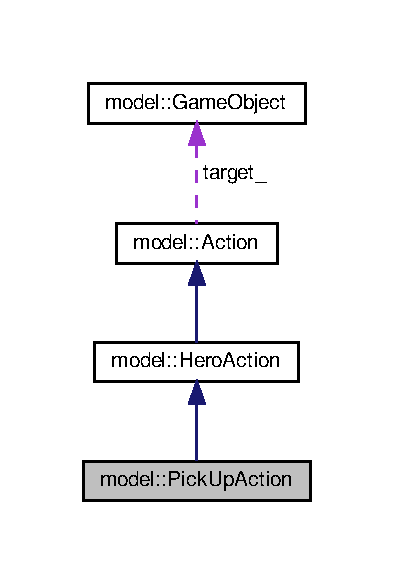
\includegraphics[width=189pt]{classmodel_1_1PickUpAction__coll__graph}
\end{center}
\end{figure}
\subsection*{Metody publiczne}
\begin{DoxyCompactItemize}
\item 
\hyperlink{classmodel_1_1PickUpAction_a7f3953e6ebdfdb1260cd745fa7fc2b8d}{Pick\+Up\+Action} (const \hyperlink{classmodel_1_1GameObject}{Game\+Object} \&target)
\begin{DoxyCompactList}\small\item\em Publiczny konstruktor z parametrem klasy \hyperlink{classmodel_1_1GameObject}{Game\+Object}. \end{DoxyCompactList}\item 
virtual void \hyperlink{classmodel_1_1PickUpAction_a8e3d6499d8eb1f99566e0b5b3e6661c9}{print} ()
\begin{DoxyCompactList}\small\item\em Wirtualna metoda print. \end{DoxyCompactList}\end{DoxyCompactItemize}
\subsection*{Dodatkowe Dziedziczone Składowe}


\subsection{Opis szczegółowy}
Klasa \hyperlink{classmodel_1_1PickUpAction}{Pick\+Up\+Action}. 

Klasa imitująca klasę akcji podniesienia danych surowców na mapie wydanego przez algorytm bota. 

\subsection{Dokumentacja konstruktora i destruktora}
\mbox{\Hypertarget{classmodel_1_1PickUpAction_a7f3953e6ebdfdb1260cd745fa7fc2b8d}\label{classmodel_1_1PickUpAction_a7f3953e6ebdfdb1260cd745fa7fc2b8d}} 
\index{model\+::\+Pick\+Up\+Action@{model\+::\+Pick\+Up\+Action}!Pick\+Up\+Action@{Pick\+Up\+Action}}
\index{Pick\+Up\+Action@{Pick\+Up\+Action}!model\+::\+Pick\+Up\+Action@{model\+::\+Pick\+Up\+Action}}
\subsubsection{\texorpdfstring{Pick\+Up\+Action()}{PickUpAction()}}
{\footnotesize\ttfamily model\+::\+Pick\+Up\+Action\+::\+Pick\+Up\+Action (\begin{DoxyParamCaption}\item[{const \hyperlink{classmodel_1_1GameObject}{Game\+Object} \&}]{target }\end{DoxyParamCaption})\hspace{0.3cm}{\ttfamily [inline]}}



Publiczny konstruktor z parametrem klasy \hyperlink{classmodel_1_1GameObject}{Game\+Object}. 


\begin{DoxyParams}{Parametry}
{\em target} & stała referencja na obiekt klasy \hyperlink{classmodel_1_1GameObject}{Game\+Object}. \\
\hline
\end{DoxyParams}


\subsection{Dokumentacja funkcji składowych}
\mbox{\Hypertarget{classmodel_1_1PickUpAction_a8e3d6499d8eb1f99566e0b5b3e6661c9}\label{classmodel_1_1PickUpAction_a8e3d6499d8eb1f99566e0b5b3e6661c9}} 
\index{model\+::\+Pick\+Up\+Action@{model\+::\+Pick\+Up\+Action}!print@{print}}
\index{print@{print}!model\+::\+Pick\+Up\+Action@{model\+::\+Pick\+Up\+Action}}
\subsubsection{\texorpdfstring{print()}{print()}}
{\footnotesize\ttfamily virtual void model\+::\+Pick\+Up\+Action\+::print (\begin{DoxyParamCaption}{ }\end{DoxyParamCaption})\hspace{0.3cm}{\ttfamily [inline]}, {\ttfamily [virtual]}}



Wirtualna metoda print. 

Stosowana jedynie do informacji o zawartości kontenera decyzji 

Reimplementowana z \hyperlink{classmodel_1_1Action_a2955dbb4a69e38a48aa07d730fe2d77c}{model\+::\+Action}.



Dokumentacja dla tej klasy została wygenerowana z pliku\+:\begin{DoxyCompactItemize}
\item 
/home/bartlomiej/eclipse-\/workspace/lab\+\_\+3/src/bot/model/\hyperlink{pick__up__action_8hpp}{pick\+\_\+up\+\_\+action.\+hpp}\end{DoxyCompactItemize}

\hypertarget{classmodel_1_1RecruitHighTierAction}{}\section{Dokumentacja klasy model\+:\+:Recruit\+High\+Tier\+Action}
\label{classmodel_1_1RecruitHighTierAction}\index{model\+::\+Recruit\+High\+Tier\+Action@{model\+::\+Recruit\+High\+Tier\+Action}}


Klasa \hyperlink{classmodel_1_1RecruitHighTierAction}{Recruit\+High\+Tier\+Action}.  




{\ttfamily \#include $<$recruit\+\_\+high\+\_\+tier\+\_\+action.\+hpp$>$}



Diagram dziedziczenia dla model\+:\+:Recruit\+High\+Tier\+Action\nopagebreak
\begin{figure}[H]
\begin{center}
\leavevmode
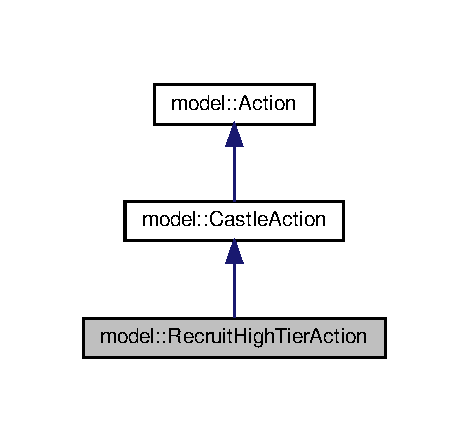
\includegraphics[width=225pt]{classmodel_1_1RecruitHighTierAction__inherit__graph}
\end{center}
\end{figure}


Diagram współpracy dla model\+:\+:Recruit\+High\+Tier\+Action\+:\nopagebreak
\begin{figure}[H]
\begin{center}
\leavevmode
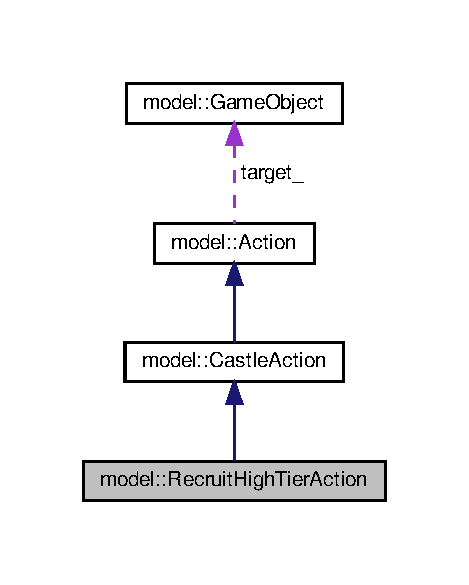
\includegraphics[width=225pt]{classmodel_1_1RecruitHighTierAction__coll__graph}
\end{center}
\end{figure}
\subsection*{Metody publiczne}
\begin{DoxyCompactItemize}
\item 
\hyperlink{classmodel_1_1RecruitHighTierAction_a470cfd0a143738a847ebf0a25e6ccd2c}{Recruit\+High\+Tier\+Action} (const \hyperlink{classmodel_1_1GameObject}{Game\+Object} \&target)
\begin{DoxyCompactList}\small\item\em Publiczny konstruktor z parametrem klasy \hyperlink{classmodel_1_1GameObject}{Game\+Object}. \end{DoxyCompactList}\item 
virtual void \hyperlink{classmodel_1_1RecruitHighTierAction_a0bedf8fdec991eff26a3eb9ffa5e552f}{print} ()
\begin{DoxyCompactList}\small\item\em Wirtualna metoda print. \end{DoxyCompactList}\end{DoxyCompactItemize}
\subsection*{Dodatkowe Dziedziczone Składowe}


\subsection{Opis szczegółowy}
Klasa \hyperlink{classmodel_1_1RecruitHighTierAction}{Recruit\+High\+Tier\+Action}. 

Klasa imitująca klasę akcji rekrutacji jednostek wysokiego poziomu wydanego przez algorytm bota. 

\subsection{Dokumentacja konstruktora i destruktora}
\mbox{\Hypertarget{classmodel_1_1RecruitHighTierAction_a470cfd0a143738a847ebf0a25e6ccd2c}\label{classmodel_1_1RecruitHighTierAction_a470cfd0a143738a847ebf0a25e6ccd2c}} 
\index{model\+::\+Recruit\+High\+Tier\+Action@{model\+::\+Recruit\+High\+Tier\+Action}!Recruit\+High\+Tier\+Action@{Recruit\+High\+Tier\+Action}}
\index{Recruit\+High\+Tier\+Action@{Recruit\+High\+Tier\+Action}!model\+::\+Recruit\+High\+Tier\+Action@{model\+::\+Recruit\+High\+Tier\+Action}}
\subsubsection{\texorpdfstring{Recruit\+High\+Tier\+Action()}{RecruitHighTierAction()}}
{\footnotesize\ttfamily model\+::\+Recruit\+High\+Tier\+Action\+::\+Recruit\+High\+Tier\+Action (\begin{DoxyParamCaption}\item[{const \hyperlink{classmodel_1_1GameObject}{Game\+Object} \&}]{target }\end{DoxyParamCaption})\hspace{0.3cm}{\ttfamily [inline]}}



Publiczny konstruktor z parametrem klasy \hyperlink{classmodel_1_1GameObject}{Game\+Object}. 


\begin{DoxyParams}{Parametry}
{\em target} & stała referencja na obiekt klasy \hyperlink{classmodel_1_1GameObject}{Game\+Object}. \\
\hline
\end{DoxyParams}


\subsection{Dokumentacja funkcji składowych}
\mbox{\Hypertarget{classmodel_1_1RecruitHighTierAction_a0bedf8fdec991eff26a3eb9ffa5e552f}\label{classmodel_1_1RecruitHighTierAction_a0bedf8fdec991eff26a3eb9ffa5e552f}} 
\index{model\+::\+Recruit\+High\+Tier\+Action@{model\+::\+Recruit\+High\+Tier\+Action}!print@{print}}
\index{print@{print}!model\+::\+Recruit\+High\+Tier\+Action@{model\+::\+Recruit\+High\+Tier\+Action}}
\subsubsection{\texorpdfstring{print()}{print()}}
{\footnotesize\ttfamily virtual void model\+::\+Recruit\+High\+Tier\+Action\+::print (\begin{DoxyParamCaption}{ }\end{DoxyParamCaption})\hspace{0.3cm}{\ttfamily [inline]}, {\ttfamily [virtual]}}



Wirtualna metoda print. 

Stosowana jedynie do informacji o zawartości kontenera decyzji 

Reimplementowana z \hyperlink{classmodel_1_1Action_a2955dbb4a69e38a48aa07d730fe2d77c}{model\+::\+Action}.



Dokumentacja dla tej klasy została wygenerowana z pliku\+:\begin{DoxyCompactItemize}
\item 
/home/bartlomiej/eclipse-\/workspace/lab\+\_\+3/src/bot/model/\hyperlink{recruit__high__tier__action_8hpp}{recruit\+\_\+high\+\_\+tier\+\_\+action.\+hpp}\end{DoxyCompactItemize}

\hypertarget{classmodel_1_1RecruitLowTierAction}{}\section{Dokumentacja klasy model\+:\+:Recruit\+Low\+Tier\+Action}
\label{classmodel_1_1RecruitLowTierAction}\index{model\+::\+Recruit\+Low\+Tier\+Action@{model\+::\+Recruit\+Low\+Tier\+Action}}


Klasa \hyperlink{classmodel_1_1RecruitLowTierAction}{Recruit\+Low\+Tier\+Action}.  




{\ttfamily \#include $<$recruit\+\_\+low\+\_\+tier\+\_\+action.\+hpp$>$}



Diagram dziedziczenia dla model\+:\+:Recruit\+Low\+Tier\+Action\nopagebreak
\begin{figure}[H]
\begin{center}
\leavevmode
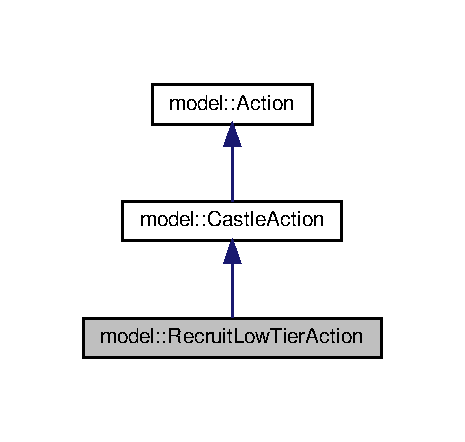
\includegraphics[width=223pt]{classmodel_1_1RecruitLowTierAction__inherit__graph}
\end{center}
\end{figure}


Diagram współpracy dla model\+:\+:Recruit\+Low\+Tier\+Action\+:\nopagebreak
\begin{figure}[H]
\begin{center}
\leavevmode
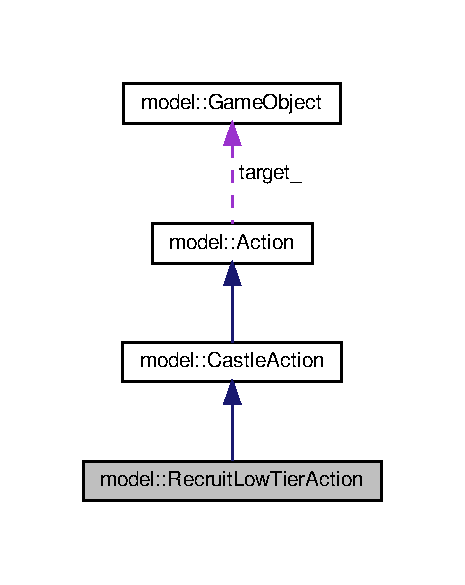
\includegraphics[width=223pt]{classmodel_1_1RecruitLowTierAction__coll__graph}
\end{center}
\end{figure}
\subsection*{Metody publiczne}
\begin{DoxyCompactItemize}
\item 
\hyperlink{classmodel_1_1RecruitLowTierAction_a15963b6d250a6a416814ed196443a533}{Recruit\+Low\+Tier\+Action} (const \hyperlink{classmodel_1_1GameObject}{Game\+Object} \&target)
\begin{DoxyCompactList}\small\item\em Publiczny konstruktor z parametrem klasy \hyperlink{classmodel_1_1GameObject}{Game\+Object}. \end{DoxyCompactList}\item 
virtual void \hyperlink{classmodel_1_1RecruitLowTierAction_ac05d2ba4872e6b06bf3a218661a4abdc}{print} ()
\begin{DoxyCompactList}\small\item\em Wirtualna metoda print. \end{DoxyCompactList}\end{DoxyCompactItemize}
\subsection*{Dodatkowe Dziedziczone Składowe}


\subsection{Opis szczegółowy}
Klasa \hyperlink{classmodel_1_1RecruitLowTierAction}{Recruit\+Low\+Tier\+Action}. 

Klasa imitująca klasę akcji rekrutacji jednostek niskiego poziomu wydanego przez algorytm bota. 

\subsection{Dokumentacja konstruktora i destruktora}
\mbox{\Hypertarget{classmodel_1_1RecruitLowTierAction_a15963b6d250a6a416814ed196443a533}\label{classmodel_1_1RecruitLowTierAction_a15963b6d250a6a416814ed196443a533}} 
\index{model\+::\+Recruit\+Low\+Tier\+Action@{model\+::\+Recruit\+Low\+Tier\+Action}!Recruit\+Low\+Tier\+Action@{Recruit\+Low\+Tier\+Action}}
\index{Recruit\+Low\+Tier\+Action@{Recruit\+Low\+Tier\+Action}!model\+::\+Recruit\+Low\+Tier\+Action@{model\+::\+Recruit\+Low\+Tier\+Action}}
\subsubsection{\texorpdfstring{Recruit\+Low\+Tier\+Action()}{RecruitLowTierAction()}}
{\footnotesize\ttfamily model\+::\+Recruit\+Low\+Tier\+Action\+::\+Recruit\+Low\+Tier\+Action (\begin{DoxyParamCaption}\item[{const \hyperlink{classmodel_1_1GameObject}{Game\+Object} \&}]{target }\end{DoxyParamCaption})\hspace{0.3cm}{\ttfamily [inline]}}



Publiczny konstruktor z parametrem klasy \hyperlink{classmodel_1_1GameObject}{Game\+Object}. 


\begin{DoxyParams}{Parametry}
{\em target} & stała referencja na obiekt klasy \hyperlink{classmodel_1_1GameObject}{Game\+Object}. \\
\hline
\end{DoxyParams}


\subsection{Dokumentacja funkcji składowych}
\mbox{\Hypertarget{classmodel_1_1RecruitLowTierAction_ac05d2ba4872e6b06bf3a218661a4abdc}\label{classmodel_1_1RecruitLowTierAction_ac05d2ba4872e6b06bf3a218661a4abdc}} 
\index{model\+::\+Recruit\+Low\+Tier\+Action@{model\+::\+Recruit\+Low\+Tier\+Action}!print@{print}}
\index{print@{print}!model\+::\+Recruit\+Low\+Tier\+Action@{model\+::\+Recruit\+Low\+Tier\+Action}}
\subsubsection{\texorpdfstring{print()}{print()}}
{\footnotesize\ttfamily virtual void model\+::\+Recruit\+Low\+Tier\+Action\+::print (\begin{DoxyParamCaption}{ }\end{DoxyParamCaption})\hspace{0.3cm}{\ttfamily [inline]}, {\ttfamily [virtual]}}



Wirtualna metoda print. 

Stosowana jedynie do informacji o zawartości kontenera decyzji 

Reimplementowana z \hyperlink{classmodel_1_1Action_a2955dbb4a69e38a48aa07d730fe2d77c}{model\+::\+Action}.



Dokumentacja dla tej klasy została wygenerowana z pliku\+:\begin{DoxyCompactItemize}
\item 
/home/bartlomiej/eclipse-\/workspace/lab\+\_\+3/src/bot/model/\hyperlink{recruit__low__tier__action_8hpp}{recruit\+\_\+low\+\_\+tier\+\_\+action.\+hpp}\end{DoxyCompactItemize}

\hypertarget{classmodel_1_1RecruitMidTierAction}{}\section{Dokumentacja klasy model\+:\+:Recruit\+Mid\+Tier\+Action}
\label{classmodel_1_1RecruitMidTierAction}\index{model\+::\+Recruit\+Mid\+Tier\+Action@{model\+::\+Recruit\+Mid\+Tier\+Action}}


Klasa \hyperlink{classmodel_1_1RecruitMidTierAction}{Recruit\+Mid\+Tier\+Action}.  




{\ttfamily \#include $<$recruit\+\_\+mid\+\_\+tier\+\_\+action.\+hpp$>$}



Diagram dziedziczenia dla model\+:\+:Recruit\+Mid\+Tier\+Action\nopagebreak
\begin{figure}[H]
\begin{center}
\leavevmode
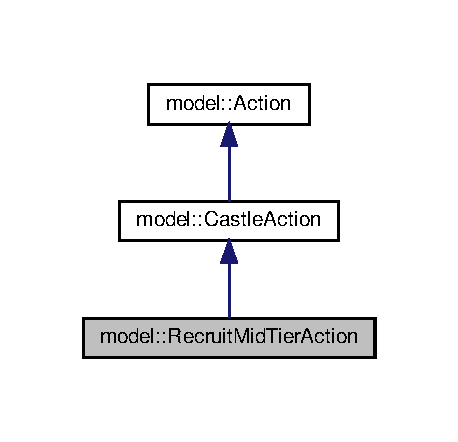
\includegraphics[width=220pt]{classmodel_1_1RecruitMidTierAction__inherit__graph}
\end{center}
\end{figure}


Diagram współpracy dla model\+:\+:Recruit\+Mid\+Tier\+Action\+:\nopagebreak
\begin{figure}[H]
\begin{center}
\leavevmode
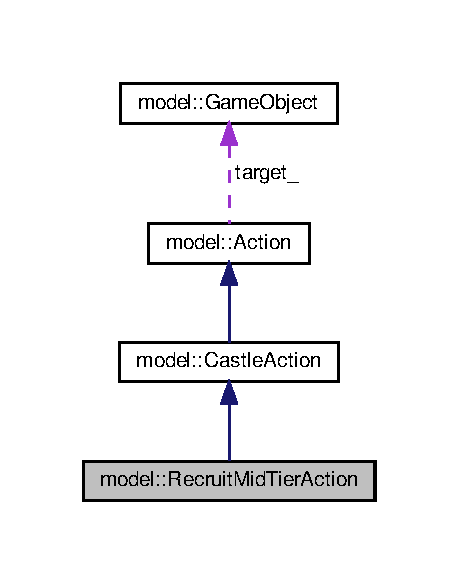
\includegraphics[width=220pt]{classmodel_1_1RecruitMidTierAction__coll__graph}
\end{center}
\end{figure}
\subsection*{Metody publiczne}
\begin{DoxyCompactItemize}
\item 
\hyperlink{classmodel_1_1RecruitMidTierAction_ad7447d08f444b49081a0294686cb47c7}{Recruit\+Mid\+Tier\+Action} (const \hyperlink{classmodel_1_1GameObject}{Game\+Object} \&target)
\begin{DoxyCompactList}\small\item\em Publiczny konstruktor z parametrem klasy \hyperlink{classmodel_1_1GameObject}{Game\+Object}. \end{DoxyCompactList}\item 
virtual void \hyperlink{classmodel_1_1RecruitMidTierAction_a91d571781540c34eea70643518e4a33d}{print} ()
\begin{DoxyCompactList}\small\item\em Wirtualna metoda print. \end{DoxyCompactList}\end{DoxyCompactItemize}
\subsection*{Dodatkowe Dziedziczone Składowe}


\subsection{Opis szczegółowy}
Klasa \hyperlink{classmodel_1_1RecruitMidTierAction}{Recruit\+Mid\+Tier\+Action}. 

Klasa imitująca klasę akcji rekrutacji jednostek średniego poziomu wydanego przez algorytm bota. 

\subsection{Dokumentacja konstruktora i destruktora}
\mbox{\Hypertarget{classmodel_1_1RecruitMidTierAction_ad7447d08f444b49081a0294686cb47c7}\label{classmodel_1_1RecruitMidTierAction_ad7447d08f444b49081a0294686cb47c7}} 
\index{model\+::\+Recruit\+Mid\+Tier\+Action@{model\+::\+Recruit\+Mid\+Tier\+Action}!Recruit\+Mid\+Tier\+Action@{Recruit\+Mid\+Tier\+Action}}
\index{Recruit\+Mid\+Tier\+Action@{Recruit\+Mid\+Tier\+Action}!model\+::\+Recruit\+Mid\+Tier\+Action@{model\+::\+Recruit\+Mid\+Tier\+Action}}
\subsubsection{\texorpdfstring{Recruit\+Mid\+Tier\+Action()}{RecruitMidTierAction()}}
{\footnotesize\ttfamily model\+::\+Recruit\+Mid\+Tier\+Action\+::\+Recruit\+Mid\+Tier\+Action (\begin{DoxyParamCaption}\item[{const \hyperlink{classmodel_1_1GameObject}{Game\+Object} \&}]{target }\end{DoxyParamCaption})\hspace{0.3cm}{\ttfamily [inline]}}



Publiczny konstruktor z parametrem klasy \hyperlink{classmodel_1_1GameObject}{Game\+Object}. 


\begin{DoxyParams}{Parametry}
{\em target} & stała referencja na obiekt klasy \hyperlink{classmodel_1_1GameObject}{Game\+Object}. \\
\hline
\end{DoxyParams}


\subsection{Dokumentacja funkcji składowych}
\mbox{\Hypertarget{classmodel_1_1RecruitMidTierAction_a91d571781540c34eea70643518e4a33d}\label{classmodel_1_1RecruitMidTierAction_a91d571781540c34eea70643518e4a33d}} 
\index{model\+::\+Recruit\+Mid\+Tier\+Action@{model\+::\+Recruit\+Mid\+Tier\+Action}!print@{print}}
\index{print@{print}!model\+::\+Recruit\+Mid\+Tier\+Action@{model\+::\+Recruit\+Mid\+Tier\+Action}}
\subsubsection{\texorpdfstring{print()}{print()}}
{\footnotesize\ttfamily virtual void model\+::\+Recruit\+Mid\+Tier\+Action\+::print (\begin{DoxyParamCaption}{ }\end{DoxyParamCaption})\hspace{0.3cm}{\ttfamily [inline]}, {\ttfamily [virtual]}}



Wirtualna metoda print. 

Stosowana jedynie do informacji o zawartości kontenera decyzji 

Reimplementowana z \hyperlink{classmodel_1_1Action_a2955dbb4a69e38a48aa07d730fe2d77c}{model\+::\+Action}.



Dokumentacja dla tej klasy została wygenerowana z pliku\+:\begin{DoxyCompactItemize}
\item 
/home/bartlomiej/eclipse-\/workspace/lab\+\_\+3/src/bot/model/\hyperlink{recruit__mid__tier__action_8hpp}{recruit\+\_\+mid\+\_\+tier\+\_\+action.\+hpp}\end{DoxyCompactItemize}

\hypertarget{classbot_1_1ScreenCapture}{}\section{Dokumentacja klasy bot\+:\+:Screen\+Capture}
\label{classbot_1_1ScreenCapture}\index{bot\+::\+Screen\+Capture@{bot\+::\+Screen\+Capture}}


Klasa \hyperlink{classbot_1_1ScreenCapture}{Screen\+Capture}.  




{\ttfamily \#include $<$screen\+\_\+capture.\+hpp$>$}

\subsection*{Metody publiczne}
\begin{DoxyCompactItemize}
\item 
\mbox{\Hypertarget{classbot_1_1ScreenCapture_a489528b1e3ab2a393801e2e712d2c998}\label{classbot_1_1ScreenCapture_a489528b1e3ab2a393801e2e712d2c998}} 
void \hyperlink{classbot_1_1ScreenCapture_a489528b1e3ab2a393801e2e712d2c998}{capture\+\_\+screen} (\hyperlink{structmodel_1_1GameState}{model\+::\+Game\+State} \&)
\begin{DoxyCompactList}\small\item\em Funkcja imitująca zbieranie danych z ekranu; faktycznie generuje stan gry losowo. \end{DoxyCompactList}\end{DoxyCompactItemize}


\subsection{Opis szczegółowy}
Klasa \hyperlink{classbot_1_1ScreenCapture}{Screen\+Capture}. 

Klasa imitująca część bota odpowiedzialną za pobieranie stanu gry z ekranu i parsowanie go do struktur rozumianych przez algorytm. Zaimplementowana by generować stan gry w sposób całkowicie losowy. 

Dokumentacja dla tej klasy została wygenerowana z plików\+:\begin{DoxyCompactItemize}
\item 
/home/bartlomiej/eclipse-\/workspace/lab\+\_\+3/src/bot/\hyperlink{screen__capture_8hpp}{screen\+\_\+capture.\+hpp}\item 
/home/bartlomiej/eclipse-\/workspace/lab\+\_\+3/src/bot/screen\+\_\+capture.\+cpp\end{DoxyCompactItemize}

\hypertarget{classmodel_1_1StatusConverter}{}\section{Dokumentacja klasy model\+:\+:Status\+Converter}
\label{classmodel_1_1StatusConverter}\index{model\+::\+Status\+Converter@{model\+::\+Status\+Converter}}


Klasa \hyperlink{classmodel_1_1StatusConverter}{Status\+Converter}.  




{\ttfamily \#include $<$status.\+hpp$>$}

\subsection*{Statyczne metody publiczne}
\begin{DoxyCompactItemize}
\item 
\mbox{\Hypertarget{classmodel_1_1StatusConverter_acbb7e3435014ae1225cc407686c52d02}\label{classmodel_1_1StatusConverter_acbb7e3435014ae1225cc407686c52d02}} 
static \hyperlink{status_8hpp_a822822ece62ee330ee656034849df887}{Status} \hyperlink{classmodel_1_1StatusConverter_acbb7e3435014ae1225cc407686c52d02}{from\+\_\+int} (int status)
\begin{DoxyCompactList}\small\item\em Statyczna publiczna fukncja konwertująca wartość całkowitą do enumeracji Status. \end{DoxyCompactList}\end{DoxyCompactItemize}


\subsection{Opis szczegółowy}
Klasa \hyperlink{classmodel_1_1StatusConverter}{Status\+Converter}. 

Dokumentacja dla tej klasy została wygenerowana z pliku\+:\begin{DoxyCompactItemize}
\item 
/home/bartlomiej/eclipse-\/workspace/lab\+\_\+3/src/bot/model/\hyperlink{status_8hpp}{status.\+hpp}\end{DoxyCompactItemize}

\hypertarget{classmodel_1_1TierConverter}{}\section{Dokumentacja klasy model\+:\+:Tier\+Converter}
\label{classmodel_1_1TierConverter}\index{model\+::\+Tier\+Converter@{model\+::\+Tier\+Converter}}


Klasa \hyperlink{classmodel_1_1TierConverter}{Tier\+Converter}.  




{\ttfamily \#include $<$tier.\+hpp$>$}

\subsection*{Statyczne metody publiczne}
\begin{DoxyCompactItemize}
\item 
\mbox{\Hypertarget{classmodel_1_1TierConverter_ab3699fb224493ff4bb99d98be4af5b9f}\label{classmodel_1_1TierConverter_ab3699fb224493ff4bb99d98be4af5b9f}} 
static \hyperlink{tier_8hpp_a50a003ab1ea342f138c038fabfd1ee55}{Tier} \hyperlink{classmodel_1_1TierConverter_ab3699fb224493ff4bb99d98be4af5b9f}{from\+\_\+int} (int tier)
\begin{DoxyCompactList}\small\item\em Statyczna publiczna fukncja konwertująca wartość całkowitą do enumeracji Tier. \end{DoxyCompactList}\end{DoxyCompactItemize}


\subsection{Opis szczegółowy}
Klasa \hyperlink{classmodel_1_1TierConverter}{Tier\+Converter}. 

Dokumentacja dla tej klasy została wygenerowana z pliku\+:\begin{DoxyCompactItemize}
\item 
/home/bartlomiej/eclipse-\/workspace/lab\+\_\+3/src/bot/model/\hyperlink{tier_8hpp}{tier.\+hpp}\end{DoxyCompactItemize}

\hypertarget{classmodel_1_1TravelToAction}{}\section{Dokumentacja klasy model\+:\+:Travel\+To\+Action}
\label{classmodel_1_1TravelToAction}\index{model\+::\+Travel\+To\+Action@{model\+::\+Travel\+To\+Action}}


Klasa \hyperlink{classmodel_1_1TravelToAction}{Travel\+To\+Action}.  




{\ttfamily \#include $<$travel\+\_\+to\+\_\+action.\+hpp$>$}



Diagram dziedziczenia dla model\+:\+:Travel\+To\+Action\nopagebreak
\begin{figure}[H]
\begin{center}
\leavevmode
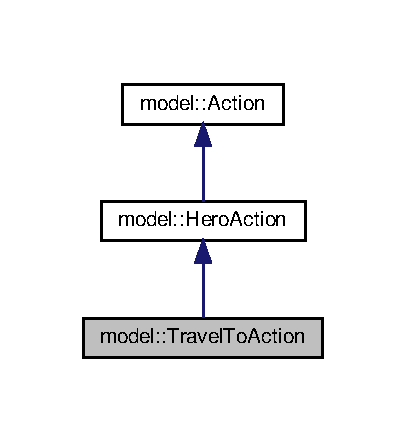
\includegraphics[width=195pt]{classmodel_1_1TravelToAction__inherit__graph}
\end{center}
\end{figure}


Diagram współpracy dla model\+:\+:Travel\+To\+Action\+:\nopagebreak
\begin{figure}[H]
\begin{center}
\leavevmode
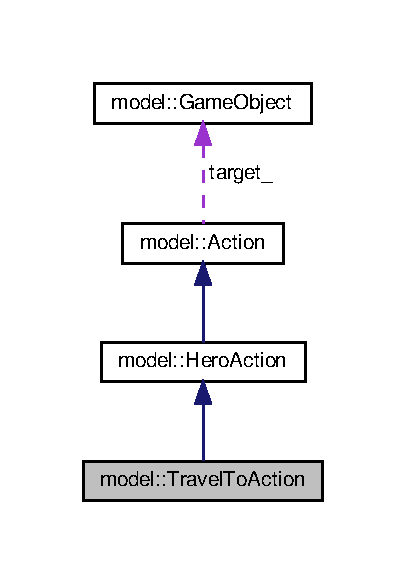
\includegraphics[width=195pt]{classmodel_1_1TravelToAction__coll__graph}
\end{center}
\end{figure}
\subsection*{Metody publiczne}
\begin{DoxyCompactItemize}
\item 
\hyperlink{classmodel_1_1TravelToAction_a5ed67f056ded96df84548a9b9e578a90}{Travel\+To\+Action} (const \hyperlink{classmodel_1_1GameObject}{Game\+Object} \&target)
\begin{DoxyCompactList}\small\item\em Publiczny konstruktor z parametrem klasy \hyperlink{classmodel_1_1GameObject}{Game\+Object}. \end{DoxyCompactList}\item 
virtual void \hyperlink{classmodel_1_1TravelToAction_accc5a7f3bf4d65e22d5d7d86624a8da1}{print} ()
\begin{DoxyCompactList}\small\item\em Wirtualna metoda print. \end{DoxyCompactList}\end{DoxyCompactItemize}
\subsection*{Dodatkowe Dziedziczone Składowe}


\subsection{Opis szczegółowy}
Klasa \hyperlink{classmodel_1_1TravelToAction}{Travel\+To\+Action}. 

Klasa imitująca klasę akcji podróżowania bohatera do danego celu wydanego przez algorytm bota. 

\subsection{Dokumentacja konstruktora i destruktora}
\mbox{\Hypertarget{classmodel_1_1TravelToAction_a5ed67f056ded96df84548a9b9e578a90}\label{classmodel_1_1TravelToAction_a5ed67f056ded96df84548a9b9e578a90}} 
\index{model\+::\+Travel\+To\+Action@{model\+::\+Travel\+To\+Action}!Travel\+To\+Action@{Travel\+To\+Action}}
\index{Travel\+To\+Action@{Travel\+To\+Action}!model\+::\+Travel\+To\+Action@{model\+::\+Travel\+To\+Action}}
\subsubsection{\texorpdfstring{Travel\+To\+Action()}{TravelToAction()}}
{\footnotesize\ttfamily model\+::\+Travel\+To\+Action\+::\+Travel\+To\+Action (\begin{DoxyParamCaption}\item[{const \hyperlink{classmodel_1_1GameObject}{Game\+Object} \&}]{target }\end{DoxyParamCaption})\hspace{0.3cm}{\ttfamily [inline]}}



Publiczny konstruktor z parametrem klasy \hyperlink{classmodel_1_1GameObject}{Game\+Object}. 


\begin{DoxyParams}{Parametry}
{\em target} & stała referencja na obiekt klasy \hyperlink{classmodel_1_1GameObject}{Game\+Object}. \\
\hline
\end{DoxyParams}


\subsection{Dokumentacja funkcji składowych}
\mbox{\Hypertarget{classmodel_1_1TravelToAction_accc5a7f3bf4d65e22d5d7d86624a8da1}\label{classmodel_1_1TravelToAction_accc5a7f3bf4d65e22d5d7d86624a8da1}} 
\index{model\+::\+Travel\+To\+Action@{model\+::\+Travel\+To\+Action}!print@{print}}
\index{print@{print}!model\+::\+Travel\+To\+Action@{model\+::\+Travel\+To\+Action}}
\subsubsection{\texorpdfstring{print()}{print()}}
{\footnotesize\ttfamily virtual void model\+::\+Travel\+To\+Action\+::print (\begin{DoxyParamCaption}{ }\end{DoxyParamCaption})\hspace{0.3cm}{\ttfamily [inline]}, {\ttfamily [virtual]}}



Wirtualna metoda print. 

Stosowana jedynie do informacji o zawartości kontenera decyzji 

Reimplementowana z \hyperlink{classmodel_1_1Action_a2955dbb4a69e38a48aa07d730fe2d77c}{model\+::\+Action}.



Dokumentacja dla tej klasy została wygenerowana z pliku\+:\begin{DoxyCompactItemize}
\item 
/home/bartlomiej/eclipse-\/workspace/lab\+\_\+3/src/bot/model/\hyperlink{travel__to__action_8hpp}{travel\+\_\+to\+\_\+action.\+hpp}\end{DoxyCompactItemize}

\hypertarget{classmodel_1_1Troop}{}\section{Dokumentacja klasy model\+:\+:Troop}
\label{classmodel_1_1Troop}\index{model\+::\+Troop@{model\+::\+Troop}}


Klasa \hyperlink{classmodel_1_1Troop}{Troop}.  




{\ttfamily \#include $<$troop.\+hpp$>$}



Diagram dziedziczenia dla model\+:\+:Troop\nopagebreak
\begin{figure}[H]
\begin{center}
\leavevmode
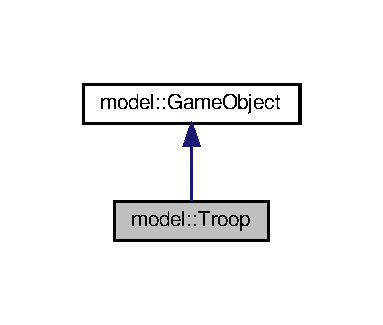
\includegraphics[width=184pt]{classmodel_1_1Troop__inherit__graph}
\end{center}
\end{figure}


Diagram współpracy dla model\+:\+:Troop\+:\nopagebreak
\begin{figure}[H]
\begin{center}
\leavevmode
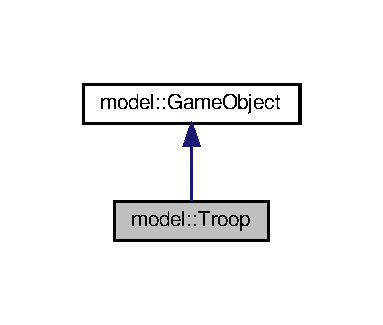
\includegraphics[width=184pt]{classmodel_1_1Troop__coll__graph}
\end{center}
\end{figure}
\subsection*{Metody publiczne}
\begin{DoxyCompactItemize}
\item 
\hyperlink{classmodel_1_1Troop_a9aa71eb10b8f3493f65dccd3d63cd7fa}{Troop} (int quantity, \hyperlink{tier_8hpp_a50a003ab1ea342f138c038fabfd1ee55}{Tier} tier, int x, int y)
\begin{DoxyCompactList}\small\item\em Publiczny konstruktor. \end{DoxyCompactList}\item 
\hyperlink{classmodel_1_1Troop_a8d7d76671d2cb6ffbd925bd91a1b4f24}{Troop} (int quantity=0, int tier=0, int x=0, int y=0)
\begin{DoxyCompactList}\small\item\em Publiczny konstruktor domyślny. \end{DoxyCompactList}\item 
\mbox{\Hypertarget{classmodel_1_1Troop_a8cbe812e8dd34a14458edca42d46a9c9}\label{classmodel_1_1Troop_a8cbe812e8dd34a14458edca42d46a9c9}} 
int \hyperlink{classmodel_1_1Troop_a8cbe812e8dd34a14458edca42d46a9c9}{get\+\_\+quantity} () const
\begin{DoxyCompactList}\small\item\em Getter zwraca liczebnośc oddziału. \end{DoxyCompactList}\item 
\mbox{\Hypertarget{classmodel_1_1Troop_afa9b13ca99af4fb5a279a01e0e2a4a7e}\label{classmodel_1_1Troop_afa9b13ca99af4fb5a279a01e0e2a4a7e}} 
\hyperlink{tier_8hpp_a50a003ab1ea342f138c038fabfd1ee55}{Tier} \hyperlink{classmodel_1_1Troop_afa9b13ca99af4fb5a279a01e0e2a4a7e}{get\+\_\+tier} () const
\begin{DoxyCompactList}\small\item\em Getter zwraca poziom oddziału. \end{DoxyCompactList}\item 
\mbox{\Hypertarget{classmodel_1_1Troop_adbec03b9cb80420608e630658bca2634}\label{classmodel_1_1Troop_adbec03b9cb80420608e630658bca2634}} 
void \hyperlink{classmodel_1_1Troop_adbec03b9cb80420608e630658bca2634}{recruit} (int quantity)
\begin{DoxyCompactList}\small\item\em Funkcja rekrutuj; zwiększa liczbę jednostek oddziału o dany parametr. \end{DoxyCompactList}\item 
\mbox{\Hypertarget{classmodel_1_1Troop_acba780ecf29542ec3f19c6090f3874d7}\label{classmodel_1_1Troop_acba780ecf29542ec3f19c6090f3874d7}} 
void \hyperlink{classmodel_1_1Troop_acba780ecf29542ec3f19c6090f3874d7}{kill} (int quantity)
\begin{DoxyCompactList}\small\item\em Funkcja zabij odejmuje zadaną liczbę jednostek z oddziału. \end{DoxyCompactList}\item 
\mbox{\Hypertarget{classmodel_1_1Troop_a1d833a9c24e879a224b84f927671b0f0}\label{classmodel_1_1Troop_a1d833a9c24e879a224b84f927671b0f0}} 
void \hyperlink{classmodel_1_1Troop_a1d833a9c24e879a224b84f927671b0f0}{vanish} ()
\begin{DoxyCompactList}\small\item\em Funkcja zabij wszystkich; ustawia liczebność oddziału na zero. \end{DoxyCompactList}\item 
\mbox{\Hypertarget{classmodel_1_1Troop_a5984aee38cb0b8982c28be8f099169db}\label{classmodel_1_1Troop_a5984aee38cb0b8982c28be8f099169db}} 
int \hyperlink{classmodel_1_1Troop_a5984aee38cb0b8982c28be8f099169db}{count\+\_\+troop\+\_\+force} () const
\begin{DoxyCompactList}\small\item\em Funkcja obliczająca siłę oddziału; mnoży jego liczebność przez współczynnik poziomu jednostek. \end{DoxyCompactList}\end{DoxyCompactItemize}
\subsection*{Statyczne atrybuty publiczne}
\begin{DoxyCompactItemize}
\item 
\mbox{\Hypertarget{classmodel_1_1Troop_a8907a194f9d0b991d2dfe43dd6136984}\label{classmodel_1_1Troop_a8907a194f9d0b991d2dfe43dd6136984}} 
static const int \hyperlink{classmodel_1_1Troop_a8907a194f9d0b991d2dfe43dd6136984}{H\+I\+G\+H\+\_\+\+T\+I\+E\+R\+\_\+\+F\+A\+C\+T\+OR} = 50
\begin{DoxyCompactList}\small\item\em Statyczna stała; współczynnik mocy jednostki wysokiego poziomu. \end{DoxyCompactList}\item 
\mbox{\Hypertarget{classmodel_1_1Troop_aedb0cd6437982a339cce8c8918d99650}\label{classmodel_1_1Troop_aedb0cd6437982a339cce8c8918d99650}} 
static const int \hyperlink{classmodel_1_1Troop_aedb0cd6437982a339cce8c8918d99650}{M\+I\+D\+\_\+\+T\+I\+E\+R\+\_\+\+F\+A\+C\+T\+OR} = 10
\begin{DoxyCompactList}\small\item\em Statyczna stała; współczynnik mocy jednostki średniego poziomu. \end{DoxyCompactList}\end{DoxyCompactItemize}


\subsection{Opis szczegółowy}
Klasa \hyperlink{classmodel_1_1Troop}{Troop}. 

Klasa oddziału w rozumieniu bota, będąca obiektem gry, więc publicznie dziedzicząca po klasie \hyperlink{classmodel_1_1GameObject}{Game\+Object}. 

\subsection{Dokumentacja konstruktora i destruktora}
\mbox{\Hypertarget{classmodel_1_1Troop_a9aa71eb10b8f3493f65dccd3d63cd7fa}\label{classmodel_1_1Troop_a9aa71eb10b8f3493f65dccd3d63cd7fa}} 
\index{model\+::\+Troop@{model\+::\+Troop}!Troop@{Troop}}
\index{Troop@{Troop}!model\+::\+Troop@{model\+::\+Troop}}
\subsubsection{\texorpdfstring{Troop()}{Troop()}\hspace{0.1cm}{\footnotesize\ttfamily [1/2]}}
{\footnotesize\ttfamily model\+::\+Troop\+::\+Troop (\begin{DoxyParamCaption}\item[{int}]{quantity,  }\item[{\hyperlink{tier_8hpp_a50a003ab1ea342f138c038fabfd1ee55}{Tier}}]{tier,  }\item[{int}]{x,  }\item[{int}]{y }\end{DoxyParamCaption})\hspace{0.3cm}{\ttfamily [inline]}}



Publiczny konstruktor. 


\begin{DoxyParams}{Parametry}
{\em quantity} & liczebność oddziału. \\
\hline
{\em tier} & poziom oddziału klasy enumeracyjnej Tier. \\
\hline
{\em x} & współrzędna x. \\
\hline
{\em y} & współrzędna y. \\
\hline
\end{DoxyParams}
\mbox{\Hypertarget{classmodel_1_1Troop_a8d7d76671d2cb6ffbd925bd91a1b4f24}\label{classmodel_1_1Troop_a8d7d76671d2cb6ffbd925bd91a1b4f24}} 
\index{model\+::\+Troop@{model\+::\+Troop}!Troop@{Troop}}
\index{Troop@{Troop}!model\+::\+Troop@{model\+::\+Troop}}
\subsubsection{\texorpdfstring{Troop()}{Troop()}\hspace{0.1cm}{\footnotesize\ttfamily [2/2]}}
{\footnotesize\ttfamily model\+::\+Troop\+::\+Troop (\begin{DoxyParamCaption}\item[{int}]{quantity = {\ttfamily 0},  }\item[{int}]{tier = {\ttfamily 0},  }\item[{int}]{x = {\ttfamily 0},  }\item[{int}]{y = {\ttfamily 0} }\end{DoxyParamCaption})\hspace{0.3cm}{\ttfamily [inline]}}



Publiczny konstruktor domyślny. 


\begin{DoxyParams}{Parametry}
{\em quantity} & liczebność oddziału. \\
\hline
{\em tier} & poziom oddziału konwetrowany do klasy enumeracyjnej Tier. \\
\hline
{\em x} & współrzędna x. \\
\hline
{\em y} & współrzędna y. \\
\hline
\end{DoxyParams}


Dokumentacja dla tej klasy została wygenerowana z pliku\+:\begin{DoxyCompactItemize}
\item 
/home/bartlomiej/eclipse-\/workspace/lab\+\_\+3/src/bot/model/\hyperlink{troop_8hpp}{troop.\+hpp}\end{DoxyCompactItemize}

\chapter{Dokumentacja plików}
\hypertarget{action__executor_8hpp}{}\section{Dokumentacja pliku /home/bartlomiej/eclipse-\/workspace/lab\+\_\+3/src/bot/action\+\_\+executor.hpp}
\label{action__executor_8hpp}\index{/home/bartlomiej/eclipse-\/workspace/lab\+\_\+3/src/bot/action\+\_\+executor.\+hpp@{/home/bartlomiej/eclipse-\/workspace/lab\+\_\+3/src/bot/action\+\_\+executor.\+hpp}}


Moduł klasy Action\+Executor.  


{\ttfamily \#include \char`\"{}model/action.\+hpp\char`\"{}}\newline
Wykres zależności załączania dla action\+\_\+executor.\+hpp\+:\nopagebreak
\begin{figure}[H]
\begin{center}
\leavevmode
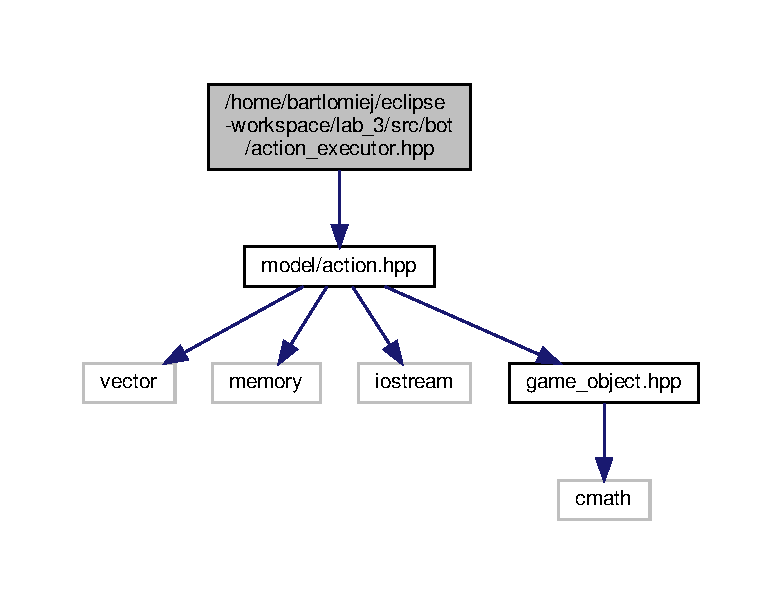
\includegraphics[width=350pt]{action__executor_8hpp__incl}
\end{center}
\end{figure}
\subsection*{Komponenty}
\begin{DoxyCompactItemize}
\item 
class \hyperlink{classbot_1_1ActionExecutor}{bot\+::\+Action\+Executor}
\begin{DoxyCompactList}\small\item\em Klasa \hyperlink{classbot_1_1ActionExecutor}{Action\+Executor}. \end{DoxyCompactList}\end{DoxyCompactItemize}


\subsection{Opis szczegółowy}
Moduł klasy Action\+Executor. 

\begin{DoxyAuthor}{Autor}
bartlomiej 
\end{DoxyAuthor}
\begin{DoxyDate}{Data}
May 12, 2019 
\end{DoxyDate}

\hypertarget{brain_8hpp}{}\section{Dokumentacja pliku /home/bartlomiej/eclipse-\/workspace/lab\+\_\+3/src/bot/brain.hpp}
\label{brain_8hpp}\index{/home/bartlomiej/eclipse-\/workspace/lab\+\_\+3/src/bot/brain.\+hpp@{/home/bartlomiej/eclipse-\/workspace/lab\+\_\+3/src/bot/brain.\+hpp}}


Moduł klasy Brain.  


{\ttfamily \#include \char`\"{}model/game\+\_\+state.\+hpp\char`\"{}}\newline
{\ttfamily \#include \char`\"{}model/action.\+hpp\char`\"{}}\newline
Wykres zależności załączania dla brain.\+hpp\+:\nopagebreak
\begin{figure}[H]
\begin{center}
\leavevmode
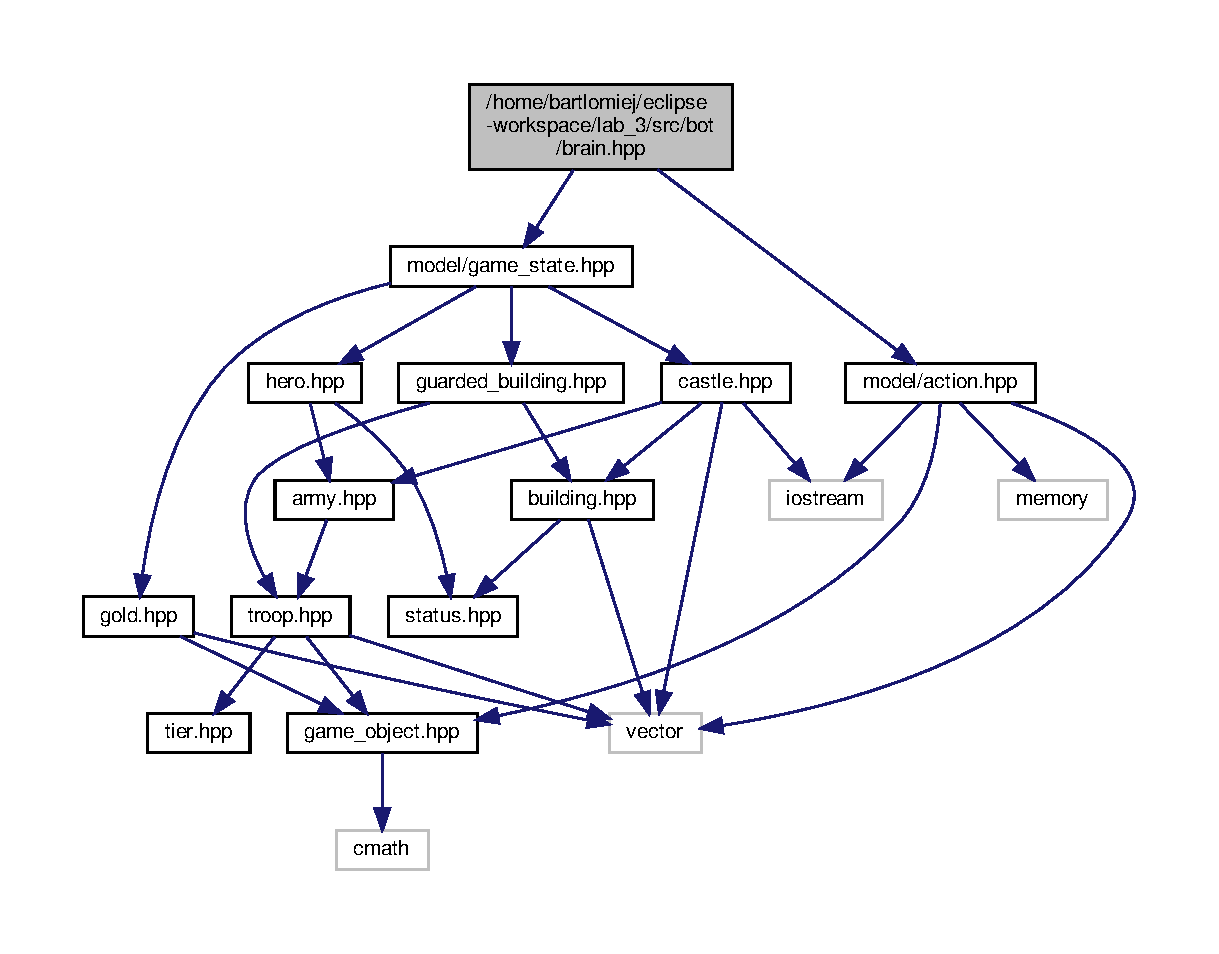
\includegraphics[width=350pt]{brain_8hpp__incl}
\end{center}
\end{figure}
\subsection*{Komponenty}
\begin{DoxyCompactItemize}
\item 
class \hyperlink{classbrain_1_1Brain}{brain\+::\+Brain}
\begin{DoxyCompactList}\small\item\em Klasa \hyperlink{classbrain_1_1Brain}{Brain}. \end{DoxyCompactList}\end{DoxyCompactItemize}


\subsection{Opis szczegółowy}
Moduł klasy Brain. 

\begin{DoxyAuthor}{Autor}
bartlomiej 
\end{DoxyAuthor}
\begin{DoxyDate}{Data}
May 12, 2019 
\end{DoxyDate}

\hypertarget{action_8hpp}{}\section{Dokumentacja pliku /home/bartlomiej/eclipse-\/workspace/lab\+\_\+3/src/bot/model/action.hpp}
\label{action_8hpp}\index{/home/bartlomiej/eclipse-\/workspace/lab\+\_\+3/src/bot/model/action.\+hpp@{/home/bartlomiej/eclipse-\/workspace/lab\+\_\+3/src/bot/model/action.\+hpp}}


Moduł klasy Action.  


{\ttfamily \#include $<$vector$>$}\newline
{\ttfamily \#include $<$memory$>$}\newline
{\ttfamily \#include $<$iostream$>$}\newline
{\ttfamily \#include \char`\"{}game\+\_\+object.\+hpp\char`\"{}}\newline
Wykres zależności załączania dla action.\+hpp\+:\nopagebreak
\begin{figure}[H]
\begin{center}
\leavevmode
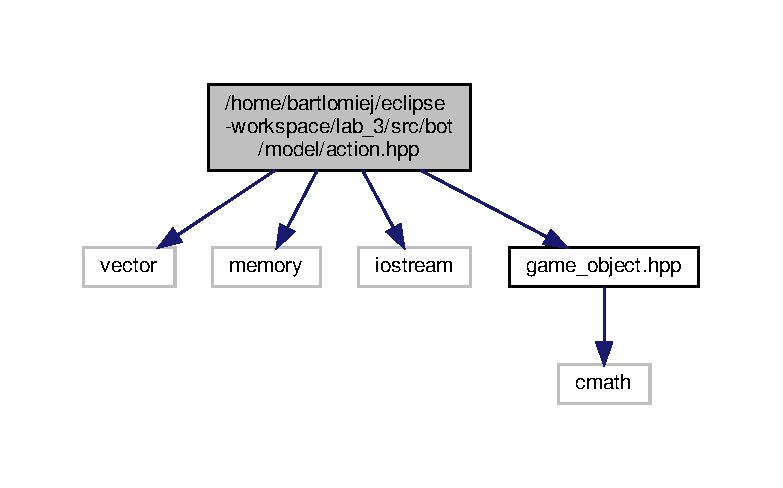
\includegraphics[width=350pt]{action_8hpp__incl}
\end{center}
\end{figure}
Ten wykres pokazuje, które pliki bezpośrednio lub pośrednio załączają ten plik\+:\nopagebreak
\begin{figure}[H]
\begin{center}
\leavevmode
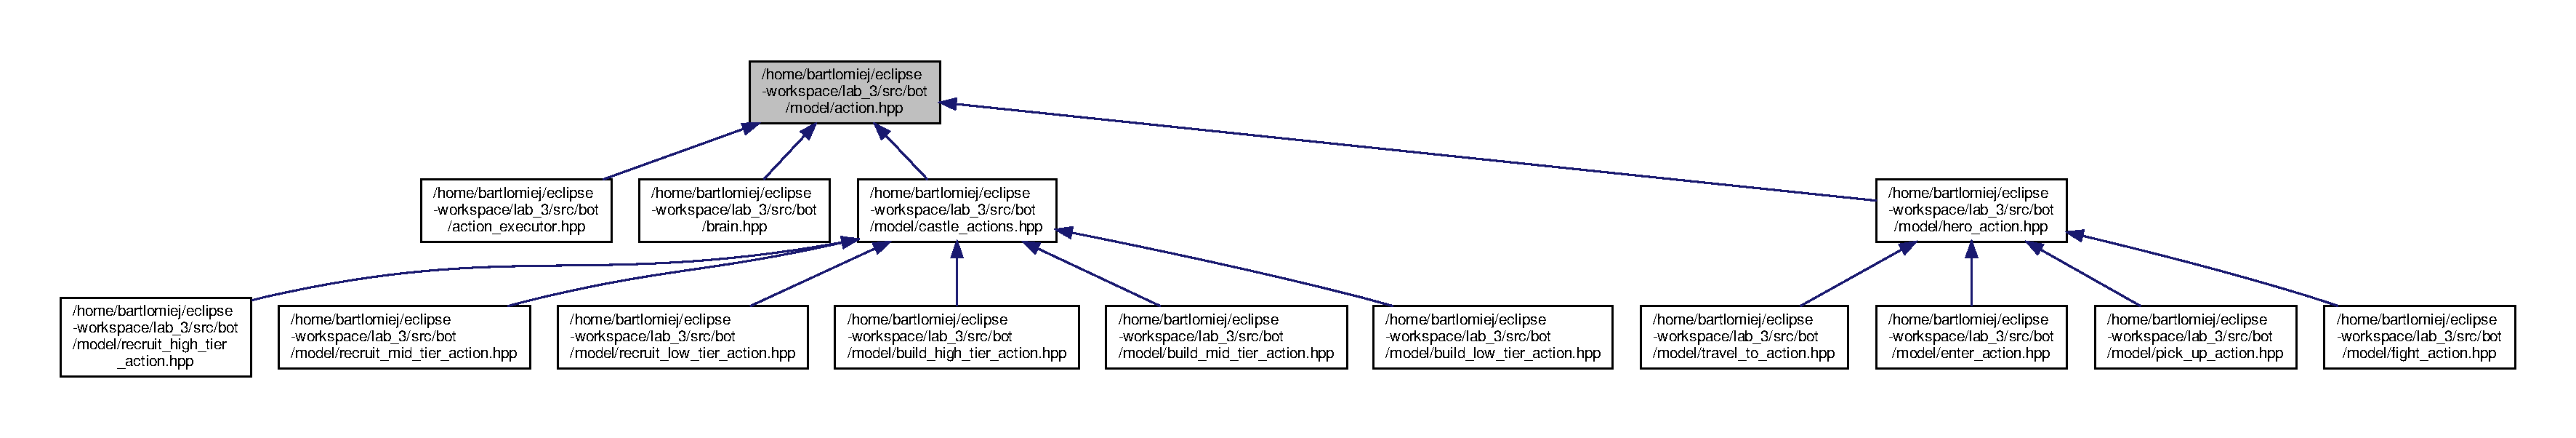
\includegraphics[width=350pt]{action_8hpp__dep__incl}
\end{center}
\end{figure}
\subsection*{Komponenty}
\begin{DoxyCompactItemize}
\item 
class \hyperlink{classmodel_1_1Action}{model\+::\+Action}
\begin{DoxyCompactList}\small\item\em Klasa \hyperlink{classmodel_1_1Action}{Action}. \end{DoxyCompactList}\end{DoxyCompactItemize}
\subsection*{Definicje typów}
\begin{DoxyCompactItemize}
\item 
\mbox{\Hypertarget{action_8hpp_a052d176abf53b10863680ac55e7ba40d}\label{action_8hpp_a052d176abf53b10863680ac55e7ba40d}} 
typedef std\+::vector$<$ std\+::unique\+\_\+ptr$<$ Action $>$ $>$ \hyperlink{action_8hpp_a052d176abf53b10863680ac55e7ba40d}{model\+::\+Action\+Scenario}
\begin{DoxyCompactList}\small\item\em Wektor inteligentnych wskaźników na klasę \hyperlink{classmodel_1_1Action}{Action} -\/ jest to zestaw decyzji bota w jednym kontenerze. \end{DoxyCompactList}\end{DoxyCompactItemize}


\subsection{Opis szczegółowy}
Moduł klasy Action. 

\begin{DoxyAuthor}{Autor}
bartlomiej 
\end{DoxyAuthor}
\begin{DoxyDate}{Data}
May 12, 2019 
\end{DoxyDate}

\hypertarget{army_8hpp}{}\section{Dokumentacja pliku /home/bartlomiej/eclipse-\/workspace/lab\+\_\+3/src/bot/model/army.hpp}
\label{army_8hpp}\index{/home/bartlomiej/eclipse-\/workspace/lab\+\_\+3/src/bot/model/army.\+hpp@{/home/bartlomiej/eclipse-\/workspace/lab\+\_\+3/src/bot/model/army.\+hpp}}


Moduł klasy Army.  


{\ttfamily \#include \char`\"{}troop.\+hpp\char`\"{}}\newline
Wykres zależności załączania dla army.\+hpp\+:\nopagebreak
\begin{figure}[H]
\begin{center}
\leavevmode
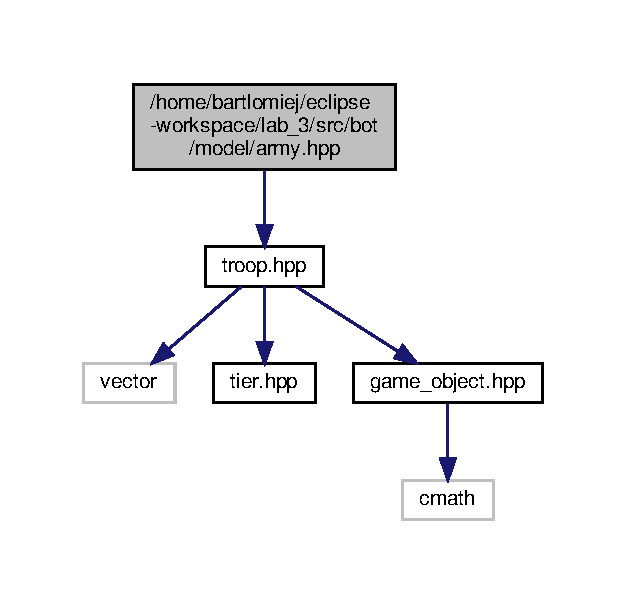
\includegraphics[width=301pt]{army_8hpp__incl}
\end{center}
\end{figure}
Ten wykres pokazuje, które pliki bezpośrednio lub pośrednio załączają ten plik\+:\nopagebreak
\begin{figure}[H]
\begin{center}
\leavevmode
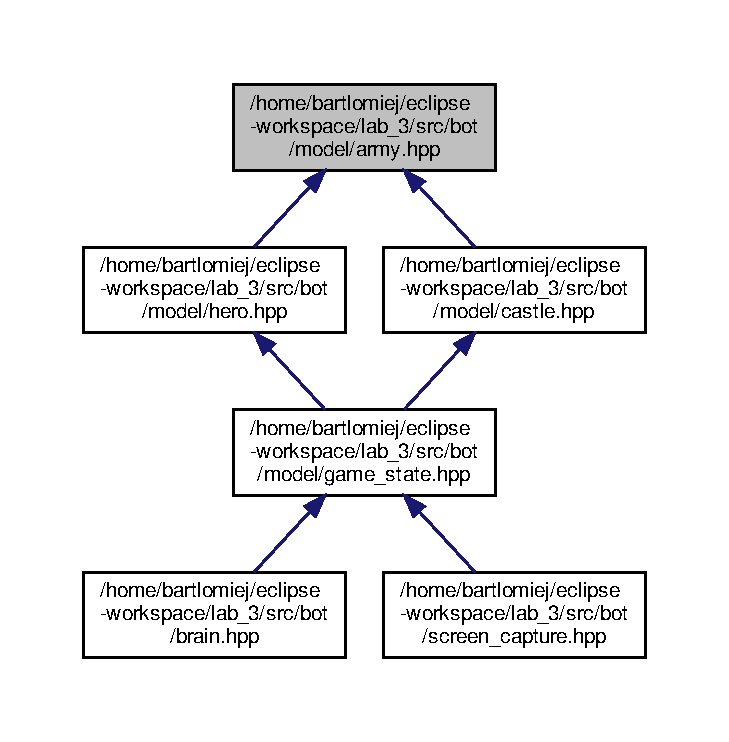
\includegraphics[width=350pt]{army_8hpp__dep__incl}
\end{center}
\end{figure}
\subsection*{Komponenty}
\begin{DoxyCompactItemize}
\item 
class \hyperlink{classmodel_1_1Army}{model\+::\+Army}
\begin{DoxyCompactList}\small\item\em Klasa \hyperlink{classmodel_1_1Army}{Army}. \end{DoxyCompactList}\end{DoxyCompactItemize}


\subsection{Opis szczegółowy}
Moduł klasy Army. 

\begin{DoxyAuthor}{Autor}
bartlomiej 
\end{DoxyAuthor}
\begin{DoxyDate}{Data}
May 12, 2019 
\end{DoxyDate}

\hypertarget{build__high__tier__action_8hpp}{}\section{Dokumentacja pliku /home/bartlomiej/eclipse-\/workspace/lab\+\_\+3/src/bot/model/build\+\_\+high\+\_\+tier\+\_\+action.hpp}
\label{build__high__tier__action_8hpp}\index{/home/bartlomiej/eclipse-\/workspace/lab\+\_\+3/src/bot/model/build\+\_\+high\+\_\+tier\+\_\+action.\+hpp@{/home/bartlomiej/eclipse-\/workspace/lab\+\_\+3/src/bot/model/build\+\_\+high\+\_\+tier\+\_\+action.\+hpp}}


Moduł klasy Build\+High\+Tier\+Action.  


{\ttfamily \#include \char`\"{}castle\+\_\+actions.\+hpp\char`\"{}}\newline
Wykres zależności załączania dla build\+\_\+high\+\_\+tier\+\_\+action.\+hpp\+:\nopagebreak
\begin{figure}[H]
\begin{center}
\leavevmode
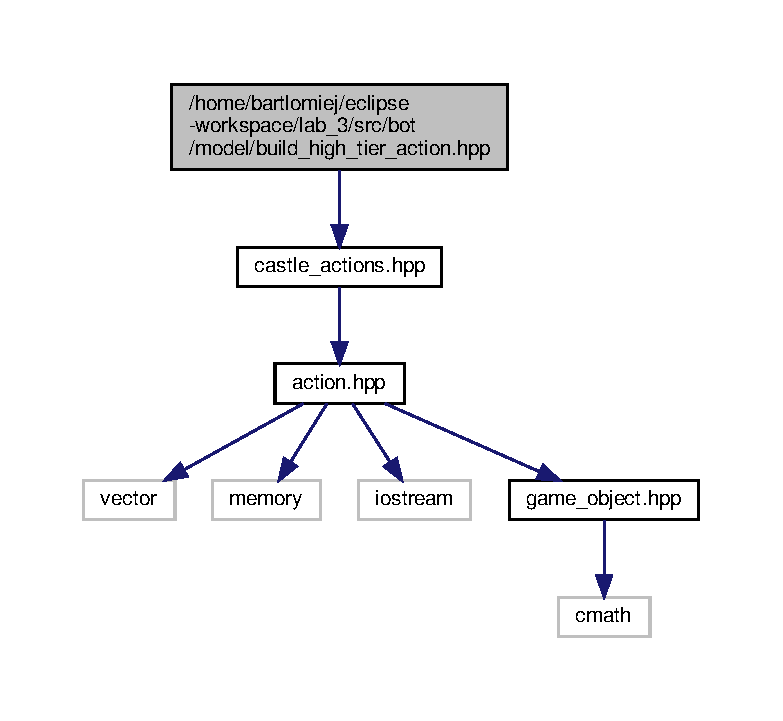
\includegraphics[width=350pt]{build__high__tier__action_8hpp__incl}
\end{center}
\end{figure}
\subsection*{Komponenty}
\begin{DoxyCompactItemize}
\item 
class \hyperlink{classmodel_1_1BuildHighTierAction}{model\+::\+Build\+High\+Tier\+Action}
\begin{DoxyCompactList}\small\item\em Klasa \hyperlink{classmodel_1_1BuildHighTierAction}{Build\+High\+Tier\+Action}. \end{DoxyCompactList}\end{DoxyCompactItemize}


\subsection{Opis szczegółowy}
Moduł klasy Build\+High\+Tier\+Action. 

\begin{DoxyAuthor}{Autor}
bartlomiej 
\end{DoxyAuthor}
\begin{DoxyDate}{Data}
May 12, 2019 
\end{DoxyDate}

\hypertarget{build__low__tier__action_8hpp}{}\section{Dokumentacja pliku /home/bartlomiej/eclipse-\/workspace/lab\+\_\+3/src/bot/model/build\+\_\+low\+\_\+tier\+\_\+action.hpp}
\label{build__low__tier__action_8hpp}\index{/home/bartlomiej/eclipse-\/workspace/lab\+\_\+3/src/bot/model/build\+\_\+low\+\_\+tier\+\_\+action.\+hpp@{/home/bartlomiej/eclipse-\/workspace/lab\+\_\+3/src/bot/model/build\+\_\+low\+\_\+tier\+\_\+action.\+hpp}}


Moduł klasy Build\+Low\+Tier\+Action.  


{\ttfamily \#include \char`\"{}castle\+\_\+actions.\+hpp\char`\"{}}\newline
Wykres zależności załączania dla build\+\_\+low\+\_\+tier\+\_\+action.\+hpp\+:\nopagebreak
\begin{figure}[H]
\begin{center}
\leavevmode
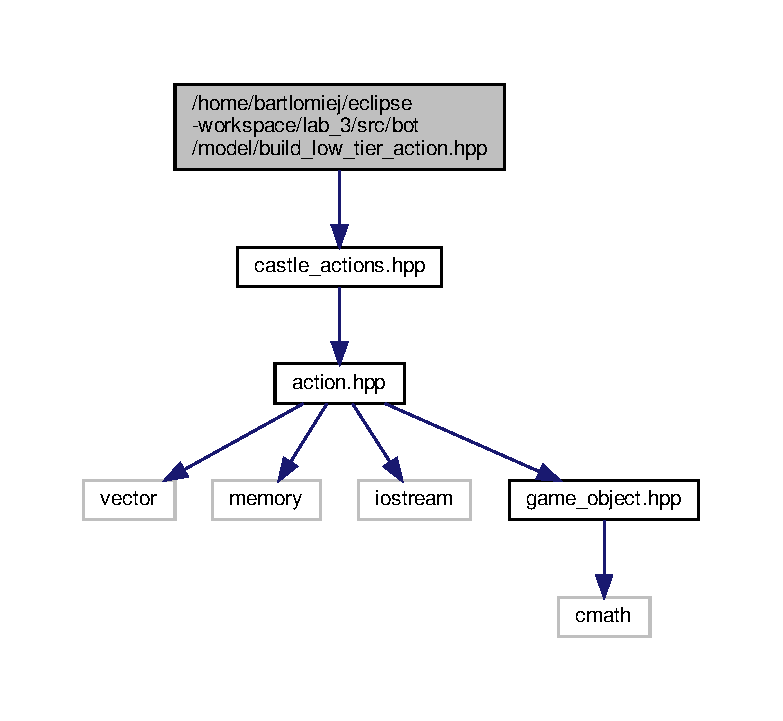
\includegraphics[width=350pt]{build__low__tier__action_8hpp__incl}
\end{center}
\end{figure}
\subsection*{Komponenty}
\begin{DoxyCompactItemize}
\item 
class \hyperlink{classmodel_1_1BuildLowTierAction}{model\+::\+Build\+Low\+Tier\+Action}
\begin{DoxyCompactList}\small\item\em Klasa \hyperlink{classmodel_1_1BuildLowTierAction}{Build\+Low\+Tier\+Action}. \end{DoxyCompactList}\end{DoxyCompactItemize}


\subsection{Opis szczegółowy}
Moduł klasy Build\+Low\+Tier\+Action. 

\begin{DoxyAuthor}{Autor}
bartlomiej 
\end{DoxyAuthor}
\begin{DoxyDate}{Data}
May 12, 2019 
\end{DoxyDate}

\hypertarget{build__mid__tier__action_8hpp}{}\section{Dokumentacja pliku /home/bartlomiej/eclipse-\/workspace/lab\+\_\+3/src/bot/model/build\+\_\+mid\+\_\+tier\+\_\+action.hpp}
\label{build__mid__tier__action_8hpp}\index{/home/bartlomiej/eclipse-\/workspace/lab\+\_\+3/src/bot/model/build\+\_\+mid\+\_\+tier\+\_\+action.\+hpp@{/home/bartlomiej/eclipse-\/workspace/lab\+\_\+3/src/bot/model/build\+\_\+mid\+\_\+tier\+\_\+action.\+hpp}}


Moduł klasy Build\+Mid\+Tier\+Action.  


{\ttfamily \#include \char`\"{}castle\+\_\+actions.\+hpp\char`\"{}}\newline
Wykres zależności załączania dla build\+\_\+mid\+\_\+tier\+\_\+action.\+hpp\+:\nopagebreak
\begin{figure}[H]
\begin{center}
\leavevmode
\includegraphics[width=350pt]{build__mid__tier__action_8hpp__incl}
\end{center}
\end{figure}
\subsection*{Komponenty}
\begin{DoxyCompactItemize}
\item 
class \hyperlink{classmodel_1_1BuildMidTierAction}{model\+::\+Build\+Mid\+Tier\+Action}
\begin{DoxyCompactList}\small\item\em Klasa \hyperlink{classmodel_1_1BuildMidTierAction}{Build\+Mid\+Tier\+Action}. \end{DoxyCompactList}\end{DoxyCompactItemize}


\subsection{Opis szczegółowy}
Moduł klasy Build\+Mid\+Tier\+Action. 

\begin{DoxyAuthor}{Autor}
bartlomiej 
\end{DoxyAuthor}
\begin{DoxyDate}{Data}
May 12, 2019 
\end{DoxyDate}

\hypertarget{building_8hpp}{}\section{Dokumentacja pliku /home/bartlomiej/eclipse-\/workspace/lab\+\_\+3/src/bot/model/building.hpp}
\label{building_8hpp}\index{/home/bartlomiej/eclipse-\/workspace/lab\+\_\+3/src/bot/model/building.\+hpp@{/home/bartlomiej/eclipse-\/workspace/lab\+\_\+3/src/bot/model/building.\+hpp}}


Moduł klasy Building.  


{\ttfamily \#include $<$vector$>$}\newline
{\ttfamily \#include \char`\"{}status.\+hpp\char`\"{}}\newline
Wykres zależności załączania dla building.\+hpp\+:\nopagebreak
\begin{figure}[H]
\begin{center}
\leavevmode
\includegraphics[width=210pt]{building_8hpp__incl}
\end{center}
\end{figure}
Ten wykres pokazuje, które pliki bezpośrednio lub pośrednio załączają ten plik\+:\nopagebreak
\begin{figure}[H]
\begin{center}
\leavevmode
\includegraphics[width=350pt]{building_8hpp__dep__incl}
\end{center}
\end{figure}
\subsection*{Komponenty}
\begin{DoxyCompactItemize}
\item 
class \hyperlink{classmodel_1_1Building}{model\+::\+Building}
\begin{DoxyCompactList}\small\item\em Klasa \hyperlink{classmodel_1_1Building}{Building}. \end{DoxyCompactList}\end{DoxyCompactItemize}
\subsection*{Definicje typów}
\begin{DoxyCompactItemize}
\item 
\mbox{\Hypertarget{building_8hpp_a73ce6a7004694882057ce332b6741811}\label{building_8hpp_a73ce6a7004694882057ce332b6741811}} 
typedef std\+::vector$<$ Building $>$ \hyperlink{building_8hpp_a73ce6a7004694882057ce332b6741811}{model\+::\+Building\+Container}
\begin{DoxyCompactList}\small\item\em Wektor budynków. \end{DoxyCompactList}\end{DoxyCompactItemize}


\subsection{Opis szczegółowy}
Moduł klasy Building. 

\begin{DoxyAuthor}{Autor}
bartlomiej 
\end{DoxyAuthor}
\begin{DoxyDate}{Data}
May 12, 2019 
\end{DoxyDate}

\hypertarget{castle_8hpp}{}\section{Dokumentacja pliku /home/bartlomiej/eclipse-\/workspace/lab\+\_\+3/src/bot/model/castle.hpp}
\label{castle_8hpp}\index{/home/bartlomiej/eclipse-\/workspace/lab\+\_\+3/src/bot/model/castle.\+hpp@{/home/bartlomiej/eclipse-\/workspace/lab\+\_\+3/src/bot/model/castle.\+hpp}}


Moduł klasy Castle.  


{\ttfamily \#include $<$vector$>$}\newline
{\ttfamily \#include $<$iostream$>$}\newline
{\ttfamily \#include \char`\"{}army.\+hpp\char`\"{}}\newline
{\ttfamily \#include \char`\"{}building.\+hpp\char`\"{}}\newline
Wykres zależności załączania dla castle.\+hpp\+:\nopagebreak
\begin{figure}[H]
\begin{center}
\leavevmode
\includegraphics[width=350pt]{castle_8hpp__incl}
\end{center}
\end{figure}
Ten wykres pokazuje, które pliki bezpośrednio lub pośrednio załączają ten plik\+:\nopagebreak
\begin{figure}[H]
\begin{center}
\leavevmode
\includegraphics[width=350pt]{castle_8hpp__dep__incl}
\end{center}
\end{figure}
\subsection*{Komponenty}
\begin{DoxyCompactItemize}
\item 
class \hyperlink{classmodel_1_1Castle}{model\+::\+Castle}
\begin{DoxyCompactList}\small\item\em Klasa \hyperlink{classmodel_1_1Castle}{Castle}. \end{DoxyCompactList}\end{DoxyCompactItemize}


\subsection{Opis szczegółowy}
Moduł klasy Castle. 

\begin{DoxyAuthor}{Autor}
bartlomiej 
\end{DoxyAuthor}
\begin{DoxyDate}{Data}
May 12, 2019 
\end{DoxyDate}

\hypertarget{castle__actions_8hpp}{}\section{Dokumentacja pliku /home/bartlomiej/eclipse-\/workspace/lab\+\_\+3/src/bot/model/castle\+\_\+actions.hpp}
\label{castle__actions_8hpp}\index{/home/bartlomiej/eclipse-\/workspace/lab\+\_\+3/src/bot/model/castle\+\_\+actions.\+hpp@{/home/bartlomiej/eclipse-\/workspace/lab\+\_\+3/src/bot/model/castle\+\_\+actions.\+hpp}}


Moduł klasy Castle\+Action.  


{\ttfamily \#include \char`\"{}action.\+hpp\char`\"{}}\newline
Wykres zależności załączania dla castle\+\_\+actions.\+hpp\+:\nopagebreak
\begin{figure}[H]
\begin{center}
\leavevmode
\includegraphics[width=350pt]{castle__actions_8hpp__incl}
\end{center}
\end{figure}
Ten wykres pokazuje, które pliki bezpośrednio lub pośrednio załączają ten plik\+:\nopagebreak
\begin{figure}[H]
\begin{center}
\leavevmode
\includegraphics[width=350pt]{castle__actions_8hpp__dep__incl}
\end{center}
\end{figure}
\subsection*{Komponenty}
\begin{DoxyCompactItemize}
\item 
class \hyperlink{classmodel_1_1CastleAction}{model\+::\+Castle\+Action}
\begin{DoxyCompactList}\small\item\em Klasa \hyperlink{classmodel_1_1CastleAction}{Castle\+Action}. \end{DoxyCompactList}\end{DoxyCompactItemize}


\subsection{Opis szczegółowy}
Moduł klasy Castle\+Action. 

\begin{DoxyAuthor}{Autor}
bartlomiej 
\end{DoxyAuthor}
\begin{DoxyDate}{Data}
May 12, 2019 
\end{DoxyDate}

\hypertarget{enter__action_8hpp}{}\section{Dokumentacja pliku /home/bartlomiej/eclipse-\/workspace/lab\+\_\+3/src/bot/model/enter\+\_\+action.hpp}
\label{enter__action_8hpp}\index{/home/bartlomiej/eclipse-\/workspace/lab\+\_\+3/src/bot/model/enter\+\_\+action.\+hpp@{/home/bartlomiej/eclipse-\/workspace/lab\+\_\+3/src/bot/model/enter\+\_\+action.\+hpp}}


Moduł klasy Enter\+Action.  


{\ttfamily \#include \char`\"{}hero\+\_\+action.\+hpp\char`\"{}}\newline
Wykres zależności załączania dla enter\+\_\+action.\+hpp\+:\nopagebreak
\begin{figure}[H]
\begin{center}
\leavevmode
\includegraphics[width=350pt]{enter__action_8hpp__incl}
\end{center}
\end{figure}
\subsection*{Komponenty}
\begin{DoxyCompactItemize}
\item 
class \hyperlink{classmodel_1_1EnterAction}{model\+::\+Enter\+Action}
\begin{DoxyCompactList}\small\item\em Klasa \hyperlink{classmodel_1_1EnterAction}{Enter\+Action}. \end{DoxyCompactList}\end{DoxyCompactItemize}


\subsection{Opis szczegółowy}
Moduł klasy Enter\+Action. 

\begin{DoxyAuthor}{Autor}
bartlomiej 
\end{DoxyAuthor}
\begin{DoxyDate}{Data}
May 12, 2019 
\end{DoxyDate}

\hypertarget{fight__action_8hpp}{}\section{Dokumentacja pliku /home/bartlomiej/eclipse-\/workspace/lab\+\_\+3/src/bot/model/fight\+\_\+action.hpp}
\label{fight__action_8hpp}\index{/home/bartlomiej/eclipse-\/workspace/lab\+\_\+3/src/bot/model/fight\+\_\+action.\+hpp@{/home/bartlomiej/eclipse-\/workspace/lab\+\_\+3/src/bot/model/fight\+\_\+action.\+hpp}}


Moduł klasy Fight\+Action.  


{\ttfamily \#include \char`\"{}hero\+\_\+action.\+hpp\char`\"{}}\newline
Wykres zależności załączania dla fight\+\_\+action.\+hpp\+:\nopagebreak
\begin{figure}[H]
\begin{center}
\leavevmode
\includegraphics[width=350pt]{fight__action_8hpp__incl}
\end{center}
\end{figure}
\subsection*{Komponenty}
\begin{DoxyCompactItemize}
\item 
class \hyperlink{classmodel_1_1FightAction}{model\+::\+Fight\+Action}
\begin{DoxyCompactList}\small\item\em Klasa \hyperlink{classmodel_1_1FightAction}{Fight\+Action}. \end{DoxyCompactList}\end{DoxyCompactItemize}


\subsection{Opis szczegółowy}
Moduł klasy Fight\+Action. 

\begin{DoxyAuthor}{Autor}
bartlomiej 
\end{DoxyAuthor}
\begin{DoxyDate}{Data}
May 12, 2019 
\end{DoxyDate}

\hypertarget{game__object_8hpp}{}\section{Dokumentacja pliku /home/bartlomiej/eclipse-\/workspace/lab\+\_\+3/src/bot/model/game\+\_\+object.hpp}
\label{game__object_8hpp}\index{/home/bartlomiej/eclipse-\/workspace/lab\+\_\+3/src/bot/model/game\+\_\+object.\+hpp@{/home/bartlomiej/eclipse-\/workspace/lab\+\_\+3/src/bot/model/game\+\_\+object.\+hpp}}


Moduł klasy Game\+Object.  


{\ttfamily \#include $<$cmath$>$}\newline
Wykres zależności załączania dla game\+\_\+object.\+hpp\+:\nopagebreak
\begin{figure}[H]
\begin{center}
\leavevmode
\includegraphics[width=206pt]{game__object_8hpp__incl}
\end{center}
\end{figure}
Ten wykres pokazuje, które pliki bezpośrednio lub pośrednio załączają ten plik\+:\nopagebreak
\begin{figure}[H]
\begin{center}
\leavevmode
\includegraphics[width=350pt]{game__object_8hpp__dep__incl}
\end{center}
\end{figure}
\subsection*{Komponenty}
\begin{DoxyCompactItemize}
\item 
class \hyperlink{classmodel_1_1GameObject}{model\+::\+Game\+Object}
\begin{DoxyCompactList}\small\item\em Klasa \hyperlink{classmodel_1_1GameObject}{Game\+Object}. \end{DoxyCompactList}\end{DoxyCompactItemize}


\subsection{Opis szczegółowy}
Moduł klasy Game\+Object. 

\begin{DoxyAuthor}{Autor}
bartlomiej 
\end{DoxyAuthor}
\begin{DoxyDate}{Data}
May 12, 2019 
\end{DoxyDate}

\hypertarget{game__state_8hpp}{}\section{Dokumentacja pliku /home/bartlomiej/eclipse-\/workspace/lab\+\_\+3/src/bot/model/game\+\_\+state.hpp}
\label{game__state_8hpp}\index{/home/bartlomiej/eclipse-\/workspace/lab\+\_\+3/src/bot/model/game\+\_\+state.\+hpp@{/home/bartlomiej/eclipse-\/workspace/lab\+\_\+3/src/bot/model/game\+\_\+state.\+hpp}}


Moduł klasy Game\+State.  


{\ttfamily \#include \char`\"{}hero.\+hpp\char`\"{}}\newline
{\ttfamily \#include \char`\"{}castle.\+hpp\char`\"{}}\newline
{\ttfamily \#include \char`\"{}guarded\+\_\+building.\+hpp\char`\"{}}\newline
{\ttfamily \#include \char`\"{}gold.\+hpp\char`\"{}}\newline
Wykres zależności załączania dla game\+\_\+state.\+hpp\+:\nopagebreak
\begin{figure}[H]
\begin{center}
\leavevmode
\includegraphics[width=350pt]{game__state_8hpp__incl}
\end{center}
\end{figure}
Ten wykres pokazuje, które pliki bezpośrednio lub pośrednio załączają ten plik\+:\nopagebreak
\begin{figure}[H]
\begin{center}
\leavevmode
\includegraphics[width=350pt]{game__state_8hpp__dep__incl}
\end{center}
\end{figure}
\subsection*{Komponenty}
\begin{DoxyCompactItemize}
\item 
struct \hyperlink{structmodel_1_1GameState}{model\+::\+Game\+State}
\begin{DoxyCompactList}\small\item\em Struktura \hyperlink{structmodel_1_1GameState}{Game\+State}. \end{DoxyCompactList}\end{DoxyCompactItemize}


\subsection{Opis szczegółowy}
Moduł klasy Game\+State. 

\begin{DoxyAuthor}{Autor}
bartlomiej 
\end{DoxyAuthor}
\begin{DoxyDate}{Data}
May 12, 2019 
\end{DoxyDate}

\hypertarget{gold_8hpp}{}\section{Dokumentacja pliku /home/bartlomiej/eclipse-\/workspace/lab\+\_\+3/src/bot/model/gold.hpp}
\label{gold_8hpp}\index{/home/bartlomiej/eclipse-\/workspace/lab\+\_\+3/src/bot/model/gold.\+hpp@{/home/bartlomiej/eclipse-\/workspace/lab\+\_\+3/src/bot/model/gold.\+hpp}}


Moduł klasy Gold.  


{\ttfamily \#include $<$vector$>$}\newline
{\ttfamily \#include \char`\"{}game\+\_\+object.\+hpp\char`\"{}}\newline
Wykres zależności załączania dla gold.\+hpp\+:\nopagebreak
\begin{figure}[H]
\begin{center}
\leavevmode
\includegraphics[width=234pt]{gold_8hpp__incl}
\end{center}
\end{figure}
Ten wykres pokazuje, które pliki bezpośrednio lub pośrednio załączają ten plik\+:\nopagebreak
\begin{figure}[H]
\begin{center}
\leavevmode
\includegraphics[width=350pt]{gold_8hpp__dep__incl}
\end{center}
\end{figure}
\subsection*{Komponenty}
\begin{DoxyCompactItemize}
\item 
class \hyperlink{classmodel_1_1Gold}{model\+::\+Gold}
\begin{DoxyCompactList}\small\item\em Klasa \hyperlink{classmodel_1_1Gold}{Gold}. \end{DoxyCompactList}\end{DoxyCompactItemize}
\subsection*{Definicje typów}
\begin{DoxyCompactItemize}
\item 
\mbox{\Hypertarget{gold_8hpp_acc4c719f33d9505529826f5d8fe38836}\label{gold_8hpp_acc4c719f33d9505529826f5d8fe38836}} 
typedef std\+::vector$<$ Gold $>$ \hyperlink{gold_8hpp_acc4c719f33d9505529826f5d8fe38836}{model\+::\+Gold\+Container}
\begin{DoxyCompactList}\small\item\em Wektor złota. \end{DoxyCompactList}\end{DoxyCompactItemize}


\subsection{Opis szczegółowy}
Moduł klasy Gold. 

\begin{DoxyAuthor}{Autor}
bartlomiej 
\end{DoxyAuthor}
\begin{DoxyDate}{Data}
May 12, 2019 
\end{DoxyDate}

\hypertarget{guarded__building_8hpp}{}\section{Dokumentacja pliku /home/bartlomiej/eclipse-\/workspace/lab\+\_\+3/src/bot/model/guarded\+\_\+building.hpp}
\label{guarded__building_8hpp}\index{/home/bartlomiej/eclipse-\/workspace/lab\+\_\+3/src/bot/model/guarded\+\_\+building.\+hpp@{/home/bartlomiej/eclipse-\/workspace/lab\+\_\+3/src/bot/model/guarded\+\_\+building.\+hpp}}


Moduł klasy Guarded\+Building.  


{\ttfamily \#include \char`\"{}building.\+hpp\char`\"{}}\newline
{\ttfamily \#include \char`\"{}troop.\+hpp\char`\"{}}\newline
Wykres zależności załączania dla guarded\+\_\+building.\+hpp\+:\nopagebreak
\begin{figure}[H]
\begin{center}
\leavevmode
\includegraphics[width=350pt]{guarded__building_8hpp__incl}
\end{center}
\end{figure}
Ten wykres pokazuje, które pliki bezpośrednio lub pośrednio załączają ten plik\+:\nopagebreak
\begin{figure}[H]
\begin{center}
\leavevmode
\includegraphics[width=350pt]{guarded__building_8hpp__dep__incl}
\end{center}
\end{figure}
\subsection*{Komponenty}
\begin{DoxyCompactItemize}
\item 
class \hyperlink{classmodel_1_1GuardedBuilding}{model\+::\+Guarded\+Building}
\begin{DoxyCompactList}\small\item\em Klasa \hyperlink{classmodel_1_1GuardedBuilding}{Guarded\+Building}. \end{DoxyCompactList}\end{DoxyCompactItemize}
\subsection*{Definicje typów}
\begin{DoxyCompactItemize}
\item 
\mbox{\Hypertarget{guarded__building_8hpp_a4c05c1c79b1b5f3bbb54b04c990d53ce}\label{guarded__building_8hpp_a4c05c1c79b1b5f3bbb54b04c990d53ce}} 
typedef std\+::vector$<$ Guarded\+Building $>$ \hyperlink{guarded__building_8hpp_a4c05c1c79b1b5f3bbb54b04c990d53ce}{model\+::\+Guarded\+Building\+Container}
\begin{DoxyCompactList}\small\item\em Wektor strzeżonych budynków. \end{DoxyCompactList}\end{DoxyCompactItemize}


\subsection{Opis szczegółowy}
Moduł klasy Guarded\+Building. 

\begin{DoxyAuthor}{Autor}
bartlomiej 
\end{DoxyAuthor}
\begin{DoxyDate}{Data}
May 12, 2019 
\end{DoxyDate}

\hypertarget{hero_8hpp}{}\section{Dokumentacja pliku /home/bartlomiej/eclipse-\/workspace/lab\+\_\+3/src/bot/model/hero.hpp}
\label{hero_8hpp}\index{/home/bartlomiej/eclipse-\/workspace/lab\+\_\+3/src/bot/model/hero.\+hpp@{/home/bartlomiej/eclipse-\/workspace/lab\+\_\+3/src/bot/model/hero.\+hpp}}


Moduł klasy Hero.  


{\ttfamily \#include \char`\"{}army.\+hpp\char`\"{}}\newline
{\ttfamily \#include \char`\"{}status.\+hpp\char`\"{}}\newline
Wykres zależności załączania dla hero.\+hpp\+:\nopagebreak
\begin{figure}[H]
\begin{center}
\leavevmode
\includegraphics[width=301pt]{hero_8hpp__incl}
\end{center}
\end{figure}
Ten wykres pokazuje, które pliki bezpośrednio lub pośrednio załączają ten plik\+:\nopagebreak
\begin{figure}[H]
\begin{center}
\leavevmode
\includegraphics[width=350pt]{hero_8hpp__dep__incl}
\end{center}
\end{figure}
\subsection*{Komponenty}
\begin{DoxyCompactItemize}
\item 
class \hyperlink{classmodel_1_1Hero}{model\+::\+Hero}
\begin{DoxyCompactList}\small\item\em Klasa \hyperlink{classmodel_1_1Hero}{Hero}. \end{DoxyCompactList}\end{DoxyCompactItemize}


\subsection{Opis szczegółowy}
Moduł klasy Hero. 

\begin{DoxyAuthor}{Autor}
bartlomiej 
\end{DoxyAuthor}
\begin{DoxyDate}{Data}
May 12, 2019 
\end{DoxyDate}

\hypertarget{hero__action_8hpp}{}\section{Dokumentacja pliku /home/bartlomiej/eclipse-\/workspace/lab\+\_\+3/src/bot/model/hero\+\_\+action.hpp}
\label{hero__action_8hpp}\index{/home/bartlomiej/eclipse-\/workspace/lab\+\_\+3/src/bot/model/hero\+\_\+action.\+hpp@{/home/bartlomiej/eclipse-\/workspace/lab\+\_\+3/src/bot/model/hero\+\_\+action.\+hpp}}


Moduł klasy Hero\+Action.  


{\ttfamily \#include \char`\"{}action.\+hpp\char`\"{}}\newline
Wykres zależności załączania dla hero\+\_\+action.\+hpp\+:\nopagebreak
\begin{figure}[H]
\begin{center}
\leavevmode
\includegraphics[width=350pt]{hero__action_8hpp__incl}
\end{center}
\end{figure}
Ten wykres pokazuje, które pliki bezpośrednio lub pośrednio załączają ten plik\+:\nopagebreak
\begin{figure}[H]
\begin{center}
\leavevmode
\includegraphics[width=350pt]{hero__action_8hpp__dep__incl}
\end{center}
\end{figure}
\subsection*{Komponenty}
\begin{DoxyCompactItemize}
\item 
class \hyperlink{classmodel_1_1HeroAction}{model\+::\+Hero\+Action}
\begin{DoxyCompactList}\small\item\em Klasa \hyperlink{classmodel_1_1HeroAction}{Hero\+Action}. \end{DoxyCompactList}\end{DoxyCompactItemize}


\subsection{Opis szczegółowy}
Moduł klasy Hero\+Action. 

\begin{DoxyAuthor}{Autor}
bartlomiej 
\end{DoxyAuthor}
\begin{DoxyDate}{Data}
May 12, 2019 
\end{DoxyDate}

\hypertarget{pick__up__action_8hpp}{}\section{Dokumentacja pliku /home/bartlomiej/eclipse-\/workspace/lab\+\_\+3/src/bot/model/pick\+\_\+up\+\_\+action.hpp}
\label{pick__up__action_8hpp}\index{/home/bartlomiej/eclipse-\/workspace/lab\+\_\+3/src/bot/model/pick\+\_\+up\+\_\+action.\+hpp@{/home/bartlomiej/eclipse-\/workspace/lab\+\_\+3/src/bot/model/pick\+\_\+up\+\_\+action.\+hpp}}


Moduł klasy Pick\+Up\+Action.  


{\ttfamily \#include \char`\"{}hero\+\_\+action.\+hpp\char`\"{}}\newline
Wykres zależności załączania dla pick\+\_\+up\+\_\+action.\+hpp\+:\nopagebreak
\begin{figure}[H]
\begin{center}
\leavevmode
\includegraphics[width=350pt]{pick__up__action_8hpp__incl}
\end{center}
\end{figure}
\subsection*{Komponenty}
\begin{DoxyCompactItemize}
\item 
class \hyperlink{classmodel_1_1PickUpAction}{model\+::\+Pick\+Up\+Action}
\begin{DoxyCompactList}\small\item\em Klasa \hyperlink{classmodel_1_1PickUpAction}{Pick\+Up\+Action}. \end{DoxyCompactList}\end{DoxyCompactItemize}


\subsection{Opis szczegółowy}
Moduł klasy Pick\+Up\+Action. 

\begin{DoxyAuthor}{Autor}
bartlomiej 
\end{DoxyAuthor}
\begin{DoxyDate}{Data}
May 12, 2019 
\end{DoxyDate}

\hypertarget{recruit__high__tier__action_8hpp}{}\section{Dokumentacja pliku /home/bartlomiej/eclipse-\/workspace/lab\+\_\+3/src/bot/model/recruit\+\_\+high\+\_\+tier\+\_\+action.hpp}
\label{recruit__high__tier__action_8hpp}\index{/home/bartlomiej/eclipse-\/workspace/lab\+\_\+3/src/bot/model/recruit\+\_\+high\+\_\+tier\+\_\+action.\+hpp@{/home/bartlomiej/eclipse-\/workspace/lab\+\_\+3/src/bot/model/recruit\+\_\+high\+\_\+tier\+\_\+action.\+hpp}}


Moduł klasy Recruit\+High\+Tier\+Action.  


{\ttfamily \#include \char`\"{}castle\+\_\+actions.\+hpp\char`\"{}}\newline
Wykres zależności załączania dla recruit\+\_\+high\+\_\+tier\+\_\+action.\+hpp\+:\nopagebreak
\begin{figure}[H]
\begin{center}
\leavevmode
\includegraphics[width=350pt]{recruit__high__tier__action_8hpp__incl}
\end{center}
\end{figure}
\subsection*{Komponenty}
\begin{DoxyCompactItemize}
\item 
class \hyperlink{classmodel_1_1RecruitHighTierAction}{model\+::\+Recruit\+High\+Tier\+Action}
\begin{DoxyCompactList}\small\item\em Klasa \hyperlink{classmodel_1_1RecruitHighTierAction}{Recruit\+High\+Tier\+Action}. \end{DoxyCompactList}\end{DoxyCompactItemize}


\subsection{Opis szczegółowy}
Moduł klasy Recruit\+High\+Tier\+Action. 

\begin{DoxyAuthor}{Autor}
bartlomiej 
\end{DoxyAuthor}
\begin{DoxyDate}{Data}
May 12, 2019 
\end{DoxyDate}

\hypertarget{recruit__low__tier__action_8hpp}{}\section{Dokumentacja pliku /home/bartlomiej/eclipse-\/workspace/lab\+\_\+3/src/bot/model/recruit\+\_\+low\+\_\+tier\+\_\+action.hpp}
\label{recruit__low__tier__action_8hpp}\index{/home/bartlomiej/eclipse-\/workspace/lab\+\_\+3/src/bot/model/recruit\+\_\+low\+\_\+tier\+\_\+action.\+hpp@{/home/bartlomiej/eclipse-\/workspace/lab\+\_\+3/src/bot/model/recruit\+\_\+low\+\_\+tier\+\_\+action.\+hpp}}


Moduł klasy Recruit\+Low\+Tier\+Action.  


{\ttfamily \#include \char`\"{}castle\+\_\+actions.\+hpp\char`\"{}}\newline
Wykres zależności załączania dla recruit\+\_\+low\+\_\+tier\+\_\+action.\+hpp\+:\nopagebreak
\begin{figure}[H]
\begin{center}
\leavevmode
\includegraphics[width=350pt]{recruit__low__tier__action_8hpp__incl}
\end{center}
\end{figure}
\subsection*{Komponenty}
\begin{DoxyCompactItemize}
\item 
class \hyperlink{classmodel_1_1RecruitLowTierAction}{model\+::\+Recruit\+Low\+Tier\+Action}
\begin{DoxyCompactList}\small\item\em Klasa \hyperlink{classmodel_1_1RecruitLowTierAction}{Recruit\+Low\+Tier\+Action}. \end{DoxyCompactList}\end{DoxyCompactItemize}


\subsection{Opis szczegółowy}
Moduł klasy Recruit\+Low\+Tier\+Action. 

\begin{DoxyAuthor}{Autor}
bartlomiej 
\end{DoxyAuthor}
\begin{DoxyDate}{Data}
May 12, 2019 
\end{DoxyDate}

\hypertarget{recruit__mid__tier__action_8hpp}{}\section{Dokumentacja pliku /home/bartlomiej/eclipse-\/workspace/lab\+\_\+3/src/bot/model/recruit\+\_\+mid\+\_\+tier\+\_\+action.hpp}
\label{recruit__mid__tier__action_8hpp}\index{/home/bartlomiej/eclipse-\/workspace/lab\+\_\+3/src/bot/model/recruit\+\_\+mid\+\_\+tier\+\_\+action.\+hpp@{/home/bartlomiej/eclipse-\/workspace/lab\+\_\+3/src/bot/model/recruit\+\_\+mid\+\_\+tier\+\_\+action.\+hpp}}


Moduł klasy Recruit\+Mid\+Tier\+Action.  


{\ttfamily \#include \char`\"{}castle\+\_\+actions.\+hpp\char`\"{}}\newline
Wykres zależności załączania dla recruit\+\_\+mid\+\_\+tier\+\_\+action.\+hpp\+:\nopagebreak
\begin{figure}[H]
\begin{center}
\leavevmode
\includegraphics[width=350pt]{recruit__mid__tier__action_8hpp__incl}
\end{center}
\end{figure}
\subsection*{Komponenty}
\begin{DoxyCompactItemize}
\item 
class \hyperlink{classmodel_1_1RecruitMidTierAction}{model\+::\+Recruit\+Mid\+Tier\+Action}
\begin{DoxyCompactList}\small\item\em Klasa \hyperlink{classmodel_1_1RecruitMidTierAction}{Recruit\+Mid\+Tier\+Action}. \end{DoxyCompactList}\end{DoxyCompactItemize}


\subsection{Opis szczegółowy}
Moduł klasy Recruit\+Mid\+Tier\+Action. 

\begin{DoxyAuthor}{Autor}
bartlomiej 
\end{DoxyAuthor}
\begin{DoxyDate}{Data}
May 12, 2019 
\end{DoxyDate}

\hypertarget{status_8hpp}{}\section{Dokumentacja pliku /home/bartlomiej/eclipse-\/workspace/lab\+\_\+3/src/bot/model/status.hpp}
\label{status_8hpp}\index{/home/bartlomiej/eclipse-\/workspace/lab\+\_\+3/src/bot/model/status.\+hpp@{/home/bartlomiej/eclipse-\/workspace/lab\+\_\+3/src/bot/model/status.\+hpp}}


Moduł klasy enumeracyjnej Status i klasy konwertera Status\+Converter.  


Ten wykres pokazuje, które pliki bezpośrednio lub pośrednio załączają ten plik\+:\nopagebreak
\begin{figure}[H]
\begin{center}
\leavevmode
\includegraphics[width=350pt]{status_8hpp__dep__incl}
\end{center}
\end{figure}
\subsection*{Komponenty}
\begin{DoxyCompactItemize}
\item 
class \hyperlink{classmodel_1_1StatusConverter}{model\+::\+Status\+Converter}
\begin{DoxyCompactList}\small\item\em Klasa \hyperlink{classmodel_1_1StatusConverter}{Status\+Converter}. \end{DoxyCompactList}\end{DoxyCompactItemize}
\subsection*{Wyliczenia}
\begin{DoxyCompactItemize}
\item 
enum \hyperlink{status_8hpp_a822822ece62ee330ee656034849df887}{model\+::\+Status} \{ {\bfseries model\+::\+Status\+::\+F\+R\+I\+E\+ND} = 0, 
{\bfseries model\+::\+Status\+::\+E\+N\+E\+MY} = 1, 
{\bfseries model\+::\+Status\+::\+N\+E\+U\+T\+R\+AL} = 2
 \}\begin{DoxyCompactList}\small\item\em Klasa enumeracyjna Status. \end{DoxyCompactList}
\end{DoxyCompactItemize}


\subsection{Opis szczegółowy}
Moduł klasy enumeracyjnej Status i klasy konwertera Status\+Converter. 

\begin{DoxyAuthor}{Autor}
bartlomiej 
\end{DoxyAuthor}
\begin{DoxyDate}{Data}
May 12, 2019 
\end{DoxyDate}


\subsection{Dokumentacja typów wyliczanych}
\mbox{\Hypertarget{status_8hpp_file_a822822ece62ee330ee656034849df887}\label{status_8hpp_file_a822822ece62ee330ee656034849df887}} 
\index{status.\+hpp@{status.\+hpp}!Status@{Status}}
\index{Status@{Status}!status.\+hpp@{status.\+hpp}}
\subsubsection{\texorpdfstring{Status}{Status}}
{\footnotesize\ttfamily enum \hyperlink{status_8hpp_a822822ece62ee330ee656034849df887}{model\+::\+Status}\hspace{0.3cm}{\ttfamily [strong]}}



Klasa enumeracyjna Status. 

Enumeracja statusu obiektów gry. 
\hypertarget{tier_8hpp}{}\section{Dokumentacja pliku /home/bartlomiej/eclipse-\/workspace/lab\+\_\+3/src/bot/model/tier.hpp}
\label{tier_8hpp}\index{/home/bartlomiej/eclipse-\/workspace/lab\+\_\+3/src/bot/model/tier.\+hpp@{/home/bartlomiej/eclipse-\/workspace/lab\+\_\+3/src/bot/model/tier.\+hpp}}


Moduł klasy enumeracyjnej Tier i klasy konwertera Tier\+Converter.  


Ten wykres pokazuje, które pliki bezpośrednio lub pośrednio załączają ten plik\+:\nopagebreak
\begin{figure}[H]
\begin{center}
\leavevmode
\includegraphics[width=350pt]{tier_8hpp__dep__incl}
\end{center}
\end{figure}
\subsection*{Komponenty}
\begin{DoxyCompactItemize}
\item 
class \hyperlink{classmodel_1_1TierConverter}{model\+::\+Tier\+Converter}
\begin{DoxyCompactList}\small\item\em Klasa \hyperlink{classmodel_1_1TierConverter}{Tier\+Converter}. \end{DoxyCompactList}\end{DoxyCompactItemize}
\subsection*{Wyliczenia}
\begin{DoxyCompactItemize}
\item 
enum \hyperlink{tier_8hpp_a50a003ab1ea342f138c038fabfd1ee55}{model\+::\+Tier} \{ {\bfseries model\+::\+Tier\+::\+L\+OW} = 0, 
{\bfseries model\+::\+Tier\+::\+M\+E\+D\+I\+UM} = 1, 
{\bfseries model\+::\+Tier\+::\+H\+I\+GH} = 2
 \}\begin{DoxyCompactList}\small\item\em Klasa enumeracyjna Tier. \end{DoxyCompactList}
\end{DoxyCompactItemize}


\subsection{Opis szczegółowy}
Moduł klasy enumeracyjnej Tier i klasy konwertera Tier\+Converter. 

\begin{DoxyAuthor}{Autor}
bartlomiej 
\end{DoxyAuthor}
\begin{DoxyDate}{Data}
May 12, 2019 
\end{DoxyDate}


\subsection{Dokumentacja typów wyliczanych}
\mbox{\Hypertarget{tier_8hpp_file_a50a003ab1ea342f138c038fabfd1ee55}\label{tier_8hpp_file_a50a003ab1ea342f138c038fabfd1ee55}} 
\index{tier.\+hpp@{tier.\+hpp}!Tier@{Tier}}
\index{Tier@{Tier}!tier.\+hpp@{tier.\+hpp}}
\subsubsection{\texorpdfstring{Tier}{Tier}}
{\footnotesize\ttfamily enum \hyperlink{tier_8hpp_a50a003ab1ea342f138c038fabfd1ee55}{model\+::\+Tier}\hspace{0.3cm}{\ttfamily [strong]}}



Klasa enumeracyjna Tier. 

Enumeracja poziomu obiektów gry. 
\hypertarget{travel__to__action_8hpp}{}\section{Dokumentacja pliku /home/bartlomiej/eclipse-\/workspace/lab\+\_\+3/src/bot/model/travel\+\_\+to\+\_\+action.hpp}
\label{travel__to__action_8hpp}\index{/home/bartlomiej/eclipse-\/workspace/lab\+\_\+3/src/bot/model/travel\+\_\+to\+\_\+action.\+hpp@{/home/bartlomiej/eclipse-\/workspace/lab\+\_\+3/src/bot/model/travel\+\_\+to\+\_\+action.\+hpp}}


Moduł klasy Travel\+To\+Action.  


{\ttfamily \#include \char`\"{}hero\+\_\+action.\+hpp\char`\"{}}\newline
Wykres zależności załączania dla travel\+\_\+to\+\_\+action.\+hpp\+:\nopagebreak
\begin{figure}[H]
\begin{center}
\leavevmode
\includegraphics[width=350pt]{travel__to__action_8hpp__incl}
\end{center}
\end{figure}
\subsection*{Komponenty}
\begin{DoxyCompactItemize}
\item 
class \hyperlink{classmodel_1_1TravelToAction}{model\+::\+Travel\+To\+Action}
\begin{DoxyCompactList}\small\item\em Klasa \hyperlink{classmodel_1_1TravelToAction}{Travel\+To\+Action}. \end{DoxyCompactList}\end{DoxyCompactItemize}


\subsection{Opis szczegółowy}
Moduł klasy Travel\+To\+Action. 

\begin{DoxyAuthor}{Autor}
bartlomiej 
\end{DoxyAuthor}
\begin{DoxyDate}{Data}
May 12, 2019 
\end{DoxyDate}

\hypertarget{troop_8hpp}{}\section{Dokumentacja pliku /home/bartlomiej/eclipse-\/workspace/lab\+\_\+3/src/bot/model/troop.hpp}
\label{troop_8hpp}\index{/home/bartlomiej/eclipse-\/workspace/lab\+\_\+3/src/bot/model/troop.\+hpp@{/home/bartlomiej/eclipse-\/workspace/lab\+\_\+3/src/bot/model/troop.\+hpp}}


Moduł klasy Troop.  


{\ttfamily \#include $<$vector$>$}\newline
{\ttfamily \#include \char`\"{}tier.\+hpp\char`\"{}}\newline
{\ttfamily \#include \char`\"{}game\+\_\+object.\+hpp\char`\"{}}\newline
Wykres zależności załączania dla troop.\+hpp\+:\nopagebreak
\begin{figure}[H]
\begin{center}
\leavevmode
\includegraphics[width=301pt]{troop_8hpp__incl}
\end{center}
\end{figure}
Ten wykres pokazuje, które pliki bezpośrednio lub pośrednio załączają ten plik\+:\nopagebreak
\begin{figure}[H]
\begin{center}
\leavevmode
\includegraphics[width=350pt]{troop_8hpp__dep__incl}
\end{center}
\end{figure}
\subsection*{Komponenty}
\begin{DoxyCompactItemize}
\item 
class \hyperlink{classmodel_1_1Troop}{model\+::\+Troop}
\begin{DoxyCompactList}\small\item\em Klasa \hyperlink{classmodel_1_1Troop}{Troop}. \end{DoxyCompactList}\end{DoxyCompactItemize}
\subsection*{Definicje typów}
\begin{DoxyCompactItemize}
\item 
\mbox{\Hypertarget{troop_8hpp_a98a8449fdd332f3100611e4f42735f26}\label{troop_8hpp_a98a8449fdd332f3100611e4f42735f26}} 
typedef std\+::vector$<$ Troop $>$ \hyperlink{troop_8hpp_a98a8449fdd332f3100611e4f42735f26}{model\+::\+Troop\+Container}
\begin{DoxyCompactList}\small\item\em Wektor oddziałów. \end{DoxyCompactList}\end{DoxyCompactItemize}


\subsection{Opis szczegółowy}
Moduł klasy Troop. 

\begin{DoxyAuthor}{Autor}
bartlomiej 
\end{DoxyAuthor}
\begin{DoxyDate}{Data}
May 12, 2019 
\end{DoxyDate}

\hypertarget{screen__capture_8hpp}{}\section{Dokumentacja pliku /home/bartlomiej/eclipse-\/workspace/lab\+\_\+3/src/bot/screen\+\_\+capture.hpp}
\label{screen__capture_8hpp}\index{/home/bartlomiej/eclipse-\/workspace/lab\+\_\+3/src/bot/screen\+\_\+capture.\+hpp@{/home/bartlomiej/eclipse-\/workspace/lab\+\_\+3/src/bot/screen\+\_\+capture.\+hpp}}


Moduł klasy Screen\+Capture.  


{\ttfamily \#include $<$vector$>$}\newline
{\ttfamily \#include $<$array$>$}\newline
{\ttfamily \#include \char`\"{}model/game\+\_\+state.\+hpp\char`\"{}}\newline
Wykres zależności załączania dla screen\+\_\+capture.\+hpp\+:\nopagebreak
\begin{figure}[H]
\begin{center}
\leavevmode
\includegraphics[width=350pt]{screen__capture_8hpp__incl}
\end{center}
\end{figure}
\subsection*{Komponenty}
\begin{DoxyCompactItemize}
\item 
class \hyperlink{classbot_1_1ScreenCapture}{bot\+::\+Screen\+Capture}
\begin{DoxyCompactList}\small\item\em Klasa \hyperlink{classbot_1_1ScreenCapture}{Screen\+Capture}. \end{DoxyCompactList}\end{DoxyCompactItemize}


\subsection{Opis szczegółowy}
Moduł klasy Screen\+Capture. 

\begin{DoxyAuthor}{Autor}
bartlomiej 
\end{DoxyAuthor}
\begin{DoxyDate}{Data}
May 12, 2019 
\end{DoxyDate}

%--- End generated contents ---

% Index
\backmatter
\newpage
\phantomsection
\clearemptydoublepage
\addcontentsline{toc}{chapter}{Indeks}
\printindex

\end{document}
